%In this section we discuss how and for what purpose the HPX backend for Blaze was modified. Our work here heavily depends on the data.
\vspace{\baselineskip}	
\section{Parallelization in Blaze}
Depending on the operation and the size of operands, this assignment could be parallelized through four different backends, namely, HPX, OpenMP\cite{dagum1998openmp}, C++ threads, and Boost\cite{Boost}. 
Table~\ref{table2} shows the default value for some of the threshold for parallelization applied to operations performed in Blaze. It should be noted that these thresholds should be tuned based on the parallelization backend and also the system architecture.
%For matrix matrix multiplication alongside the mentioned thresholds, there exists another set of thresholds to switch between using Blaze kernels or BLAS kernels. 
%As stated in Section~\ref{Background} Blaze being based on smart expression templates, offers the option to use either Blaze or a highly optimized kernel for computations. This option is set at compile time through $BLAS_mode$ macro. If $BLAS_mode=1$, 

\vspace{\baselineskip}	
\begin{table}[H]
	\centering
	\resizebox{\textwidth}{!}
	{\begin{tabular}{|c | c |} 
			\hline
			Benchmark & Array size \\ [0.5ex] 
			\hline
			\hline
			$DVECDVCEADD$, $DVECDVECMULT$ & 38000\\ 	
			\hline
			$DMATDMATADD$ & 36100 elements equivalent to a $175\times{175}$ matrix \\
			\hline	
			$DMATDMATMULT$ & 3025 elements equivalent to a $55\times{55}$ matrix  \\
			\hline			
	\end{tabular}}
	
	\caption{List of some of the thresholds applied to the operations performed by Blaze, starting from which the operation is executed in parallel}
	\label{table2}
\end{table} 

\vspace{\baselineskip}	
\subsection{Implementation of HPX Backend}
As stated earlier, as an ET-based library, blaze performs the calculations when an expression is assigned to a target, which is implemented through the \textit{blaze::Assign} function.

The four mentioned backends, parallelize this assignment process through a parallel for-loop, in which at each iteration a specific section of each of the vectors or matrices(called a block) is selected and assigned to a core. Each core then performs the operation on the block they have been assigned to.  

Each backend uses their own method for parallelizing this for loop. For HPX backend, current implementation uses a HPX \textit{parallel::for\textunderscore loop} with static chunking policy and chunk size of 1. This way, knowing the number of cores to run the application on, we can divide the original matrix equally among the cores, while the order of assignment of blocks to the cores is known at compile time.  
Listings\ref{old_hpx_backend} shows the current implementation of the HPX backend in Blaze.

\begin{lstlisting}[float,floatplacement=H,caption= {Previous implementation of Assign function for HPX backend in Blaze.}, label={old_hpx_backend}]
template< typename MT1   // Type of the left-hand side dense matrix
, bool SO1       // Storage order of the left-hand side dense matrix
, typename MT2   // Type of the right-hand side dense matrix
, bool SO2       // Storage order of the right-hand side dense matrix
, typename OP >  // Type of the assignment operation
void hpxAssign( DenseMatrix<MT1,SO1>& lhs, const DenseMatrix<MT2,SO2>& rhs, OP op )
{
using hpx::parallel::for_loop;
using hpx::parallel::execution::par;

BLAZE_FUNCTION_TRACE;

using ET1 = ElementType_t<MT1>;
using ET2 = ElementType_t<MT2>;

constexpr bool simdEnabled( MT1::simdEnabled && MT2::simdEnabled && IsSIMDCombinable_v<ET1,ET2> );
constexpr size_t SIMDSIZE( SIMDTrait< ElementType_t<MT1> >::size );

const bool lhsAligned( (~lhs).isAligned() );
const bool rhsAligned( (~rhs).isAligned() );

const size_t threads    ( getNumThreads() );
const ThreadMapping threadmap( createThreadMapping( threads, ~rhs ) );

const size_t addon1     ( ( ( (~rhs).rows() % threadmap.first ) != 0UL )? 1UL : 0UL );
const size_t equalShare1( (~rhs).rows() / threadmap.first + addon1 );
const size_t rest1      ( equalShare1 & ( SIMDSIZE - 1UL ) );
const size_t rowsPerThread( ( simdEnabled && rest1 )?( equalShare1 - rest1 + SIMDSIZE ):( equalShare1 ) );

const size_t addon2     ( ( ( (~rhs).columns() % threadmap.second ) != 0UL )? 1UL : 0UL );
const size_t equalShare2( (~rhs).columns() / threadmap.second + addon2 );
const size_t rest2      ( equalShare2 & ( SIMDSIZE - 1UL ) );
const size_t colsPerThread( ( simdEnabled && rest2 )?( equalShare2 - rest2 + SIMDSIZE ):( equalShare2 ) );

for_loop( par, size_t(0), threads, [&](int i)
{
const size_t row   ( ( i / threadmap.second ) * rowsPerThread );
const size_t column( ( i % threadmap.second ) * colsPerThread );

if( row >= (~rhs).rows() || column >= (~rhs).columns() )
return;

const size_t m( min( rowsPerThread, (~rhs).rows()    - row    ) );
const size_t n( min( colsPerThread, (~rhs).columns() - column ) );

if( simdEnabled && lhsAligned && rhsAligned ) {
auto       target( submatrix<aligned>( ~lhs, row, column, m, n ) );
const auto source( submatrix<aligned>( ~rhs, row, column, m, n ) );
op( target, source );
}
else if( simdEnabled && lhsAligned ) {
auto       target( submatrix<aligned>( ~lhs, row, column, m, n ) );
const auto source( submatrix<unaligned>( ~rhs, row, column, m, n ) );
op( target, source );
}
else if( simdEnabled && rhsAligned ) {
auto       target( submatrix<unaligned>( ~lhs, row, column, m, n ) );
const auto source( submatrix<aligned>( ~rhs, row, column, m, n ) );
op( target, source );
}
else {
auto       target( submatrix<unaligned>( ~lhs, row, column, m, n ) );
const auto source( submatrix<unaligned>( ~rhs, row, column, m, n ) );
op( target, source );
}
} );
}
\end{lstlisting}

What we suggest here is that, some prior knowledge for example, architecture of the system we are running the application on, the expression that has to be executed, number of cores of the system, size and type of the arrays we are dealing with, and etc. should be able to help us to achieve a higher performance.
For this purpose we introduced two parameters block\textunderscore{size} and chunk\textunderscore{size}.

\begin{lstlisting}[float,floatplacement=H,caption= {New implementation of Assign function for HPX backend in Blaze.}, label={new_hpx_backend}]
template< typename MT1   // Type of the left-hand side dense matrix
, bool SO1       // Storage order of the left-hand side dense matrix
, typename MT2   // Type of the right-hand side dense matrix
, bool SO2       // Storage order of the right-hand side dense matrix
, typename OP >  // Type of the assignment operation
void hpxAssign( DenseMatrix<MT1,SO1>& lhs, const DenseMatrix<MT2,SO2>& rhs, OP op )
{
using hpx::parallel::for_loop;
using hpx::parallel::execution::par;

BLAZE_FUNCTION_TRACE;

using ET1 = ElementType_t<MT1>;
using ET2 = ElementType_t<MT2>;

constexpr bool simdEnabled( MT1::simdEnabled && MT2::simdEnabled && IsSIMDCombinable_v<ET1,ET2> );
constexpr size_t SIMDSIZE( SIMDTrait< ElementType_t<MT1> >::size );

const bool lhsAligned( (~lhs).isAligned() );
const bool rhsAligned( (~rhs).isAligned() );

const size_t threads    ( getNumThreads() );
const size_t numRows ( min( static_cast<std::size_t>( BLAZE_HPX_MATRIX_BLOCK_SIZE_ROW ), (~rhs).rows() ) );
const size_t numCols ( min( static_cast<std::size_t>( BLAZE_HPX_MATRIX_BLOCK_SIZE_COLUMN ), (~rhs).columns() ) );

const size_t rest1      ( numRows & ( SIMDSIZE - 1UL ) );
const size_t rowsPerIter( ( simdEnabled && rest1 )?( numRows - rest1 + SIMDSIZE ):( numRows ) );
const size_t addon1     ( ( ( (~rhs).rows() % rowsPerIter ) != 0UL )? 1UL : 0UL );
const size_t equalShare1( (~rhs).rows() / rowsPerIter + addon1 );

const size_t rest2      ( numCols & ( SIMDSIZE - 1UL ) );
const size_t colsPerIter( ( simdEnabled && rest2 )?( numCols - rest2 + SIMDSIZE ):( numCols ) );
const size_t addon2     ( ( ( (~rhs).columns() % colsPerIter ) != 0UL )? 1UL : 0UL );
const size_t equalShare2( (~rhs).columns() / colsPerIter + addon2 );

hpx::parallel::execution::dynamic_chunk_size chunkSize ( BLAZE_HPX_MATRIX_CHUNK_SIZE );

for_loop( par.with( chunkSize ), size_t(0), equalShare1 * equalShare2, [&](int i)
{
const size_t row   ( ( i / equalShare2 ) * rowsPerIter );
const size_t column( ( i % equalShare2 ) * colsPerIter );

if( row >= (~rhs).rows() || column >= (~rhs).columns() )
return;

const size_t m( min( rowsPerIter, (~rhs).rows()    - row    ) );
const size_t n( min( colsPerIter, (~rhs).columns() - column ) );

if( simdEnabled && lhsAligned && rhsAligned ) {
auto       target( submatrix<aligned>( ~lhs, row, column, m, n ) );
const auto source( submatrix<aligned>( ~rhs, row, column, m, n ) );
op( target, source );
}
else if( simdEnabled && lhsAligned ) {
auto       target( submatrix<aligned>( ~lhs, row, column, m, n ) );
const auto source( submatrix<unaligned>( ~rhs, row, column, m, n ) );
op( target, source );
}
else if( simdEnabled && rhsAligned ) {
auto       target( submatrix<unaligned>( ~lhs, row, column, m, n ) );
const auto source( submatrix<aligned>( ~rhs, row, column, m, n ) );
op( target, source );
}
else {
auto       target( submatrix<unaligned>( ~lhs, row, column, m, n ) );
const auto source( submatrix<unaligned>( ~rhs, row, column, m, n ) );
op( target, source );
}
} );
}
\end{lstlisting}
\vspace{\baselineskip}	
\subsection{HPX \textit{for\textunderscore loop}}
HPX \textit{for\textunderscore loop} takes an execution policy as first argument, which is set to \textit{dynamic\textunderscore chunk\textunderscore size} execution policy in case of HPX backend for Blaze.

\vspace{\baselineskip}	
\section{Experiments}
In order to capture the relationship between number of cores, \textit{chunk\textunderscore{size}}, \textit{block\textunderscore{size}}, and the performance, we ran a series of experiments with different of these parameters and measured the number of floating point operations per second performed. 

For these experiments ,at the first step we selected the $DMatDMatADD$ benchmark which was implemented in Blazemark. $DMatDMatADD$ benchmark is a level 3 BLAS function to perform matrix-matrix addition in the form of $A=B+C$, where $A$, $B$, $C$ are square matrices of the same size. 

To avoid adding the scheduling overhead for small matrix sizes, Blaze uses a threshold to start parallelization, which is specific to the type of operation. For matrix-matrix addition, if the number of elements in the matrix is greater than 36100 elements(which is equivalent to a square matrix of size 190$\times$190) Blaze uses the configured backend to parallelize the assignment operation. For this reason, we start our experiments with matrix size of 200x200 and gradually increase the size to 1587$\times$1587. 
Table~\ref{table1} show the matrix sizes and the number of cores chosen for our experiments with $DMATDMATADD$ benchmark.

\vspace{\baselineskip}	
\begin{table}[H]
	\centering
		\resizebox{\textwidth}{!}
		{\begin{tabular}{|c | c |} 
			\hline
			Matrix sizes & 200, 230, 264, 300, 396, 455, 523, 600, 690, 793, 912, 1048, 1200, 1380, 1587 \\ [0.5ex] 
			\hline
			Number of cores & 1, 2, 3, 4, 5, 6, 7, 8 \\ 	
			\hline
			Number of rows in the block & 4, 8, 12, 16, 20, 32 \\
			\hline	
			Number of columns in the block & 64, 128, 256, 512, 1024 \\
			\hline
			Chunk size & Between 1 and total number of blocks (logarithmic increase)\\\hline
		\end{tabular}}

		\caption{List of different values used for each variable for running the $DMATDMATADD$ benchmark}
		\label{table1}
\end{table}

\vspace{\baselineskip}	
Figure~\ref{fig1} shows the results of running $DMatDMatADD$ benchmark for matrix sizes and number of cores listed in Tbale~\ref{table1} based on grain size. 

On the other hand, Figure~\ref{fig4} integrates the results obtained from running the same benchmark with different matrix sizes. Each color in this graph represents a specific matrix size. 

\vspace{\baselineskip}	
\begin{figure}[H]
	\centering
	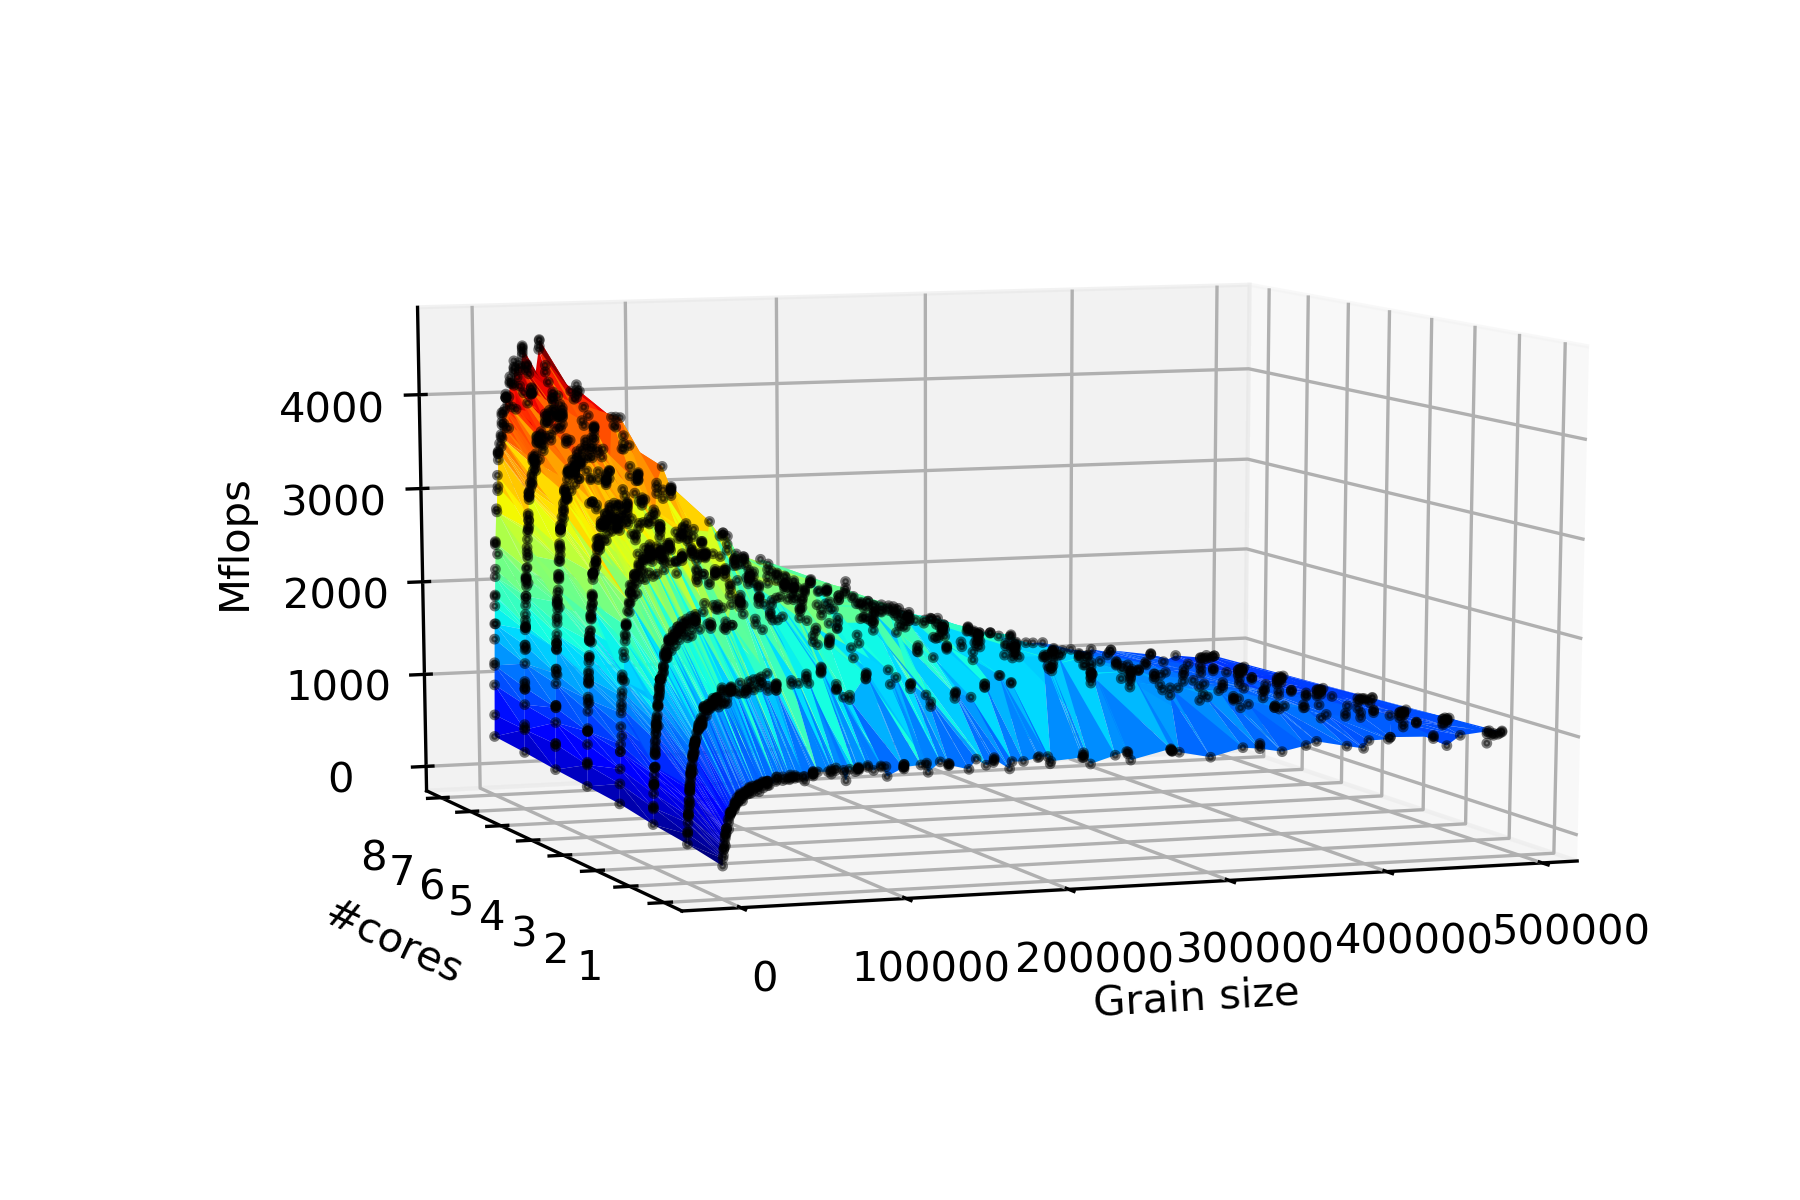
\includegraphics[width=1\linewidth]{images/fig2.png}
	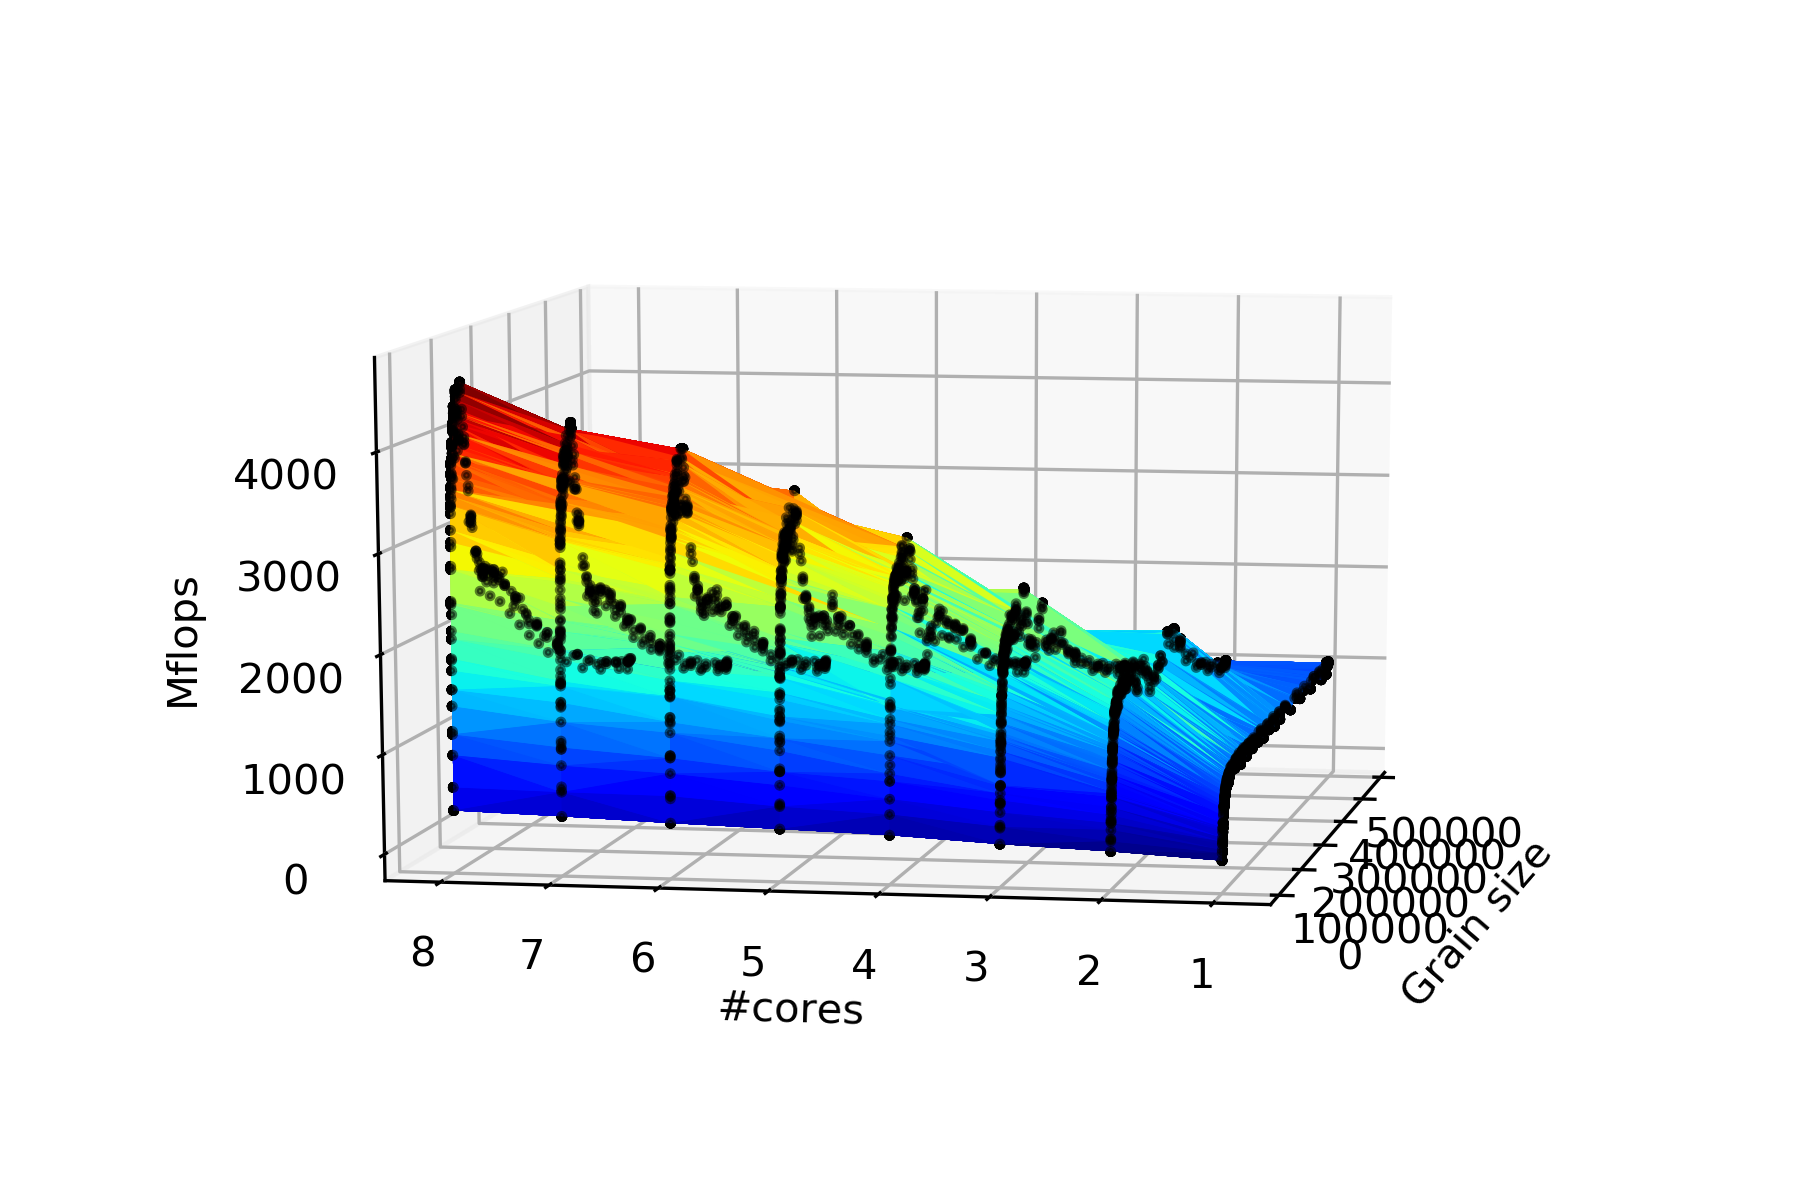
\includegraphics[width=1\linewidth]{images/fig3.png}
	\caption{The results obtained from running $DMATDMATADD$ benchmark through Blazemark for matrix of size 690$\times$690 from two different angles}	
	\label{fig1}
\end{figure}

\begin{figure}[H]
	\centering
	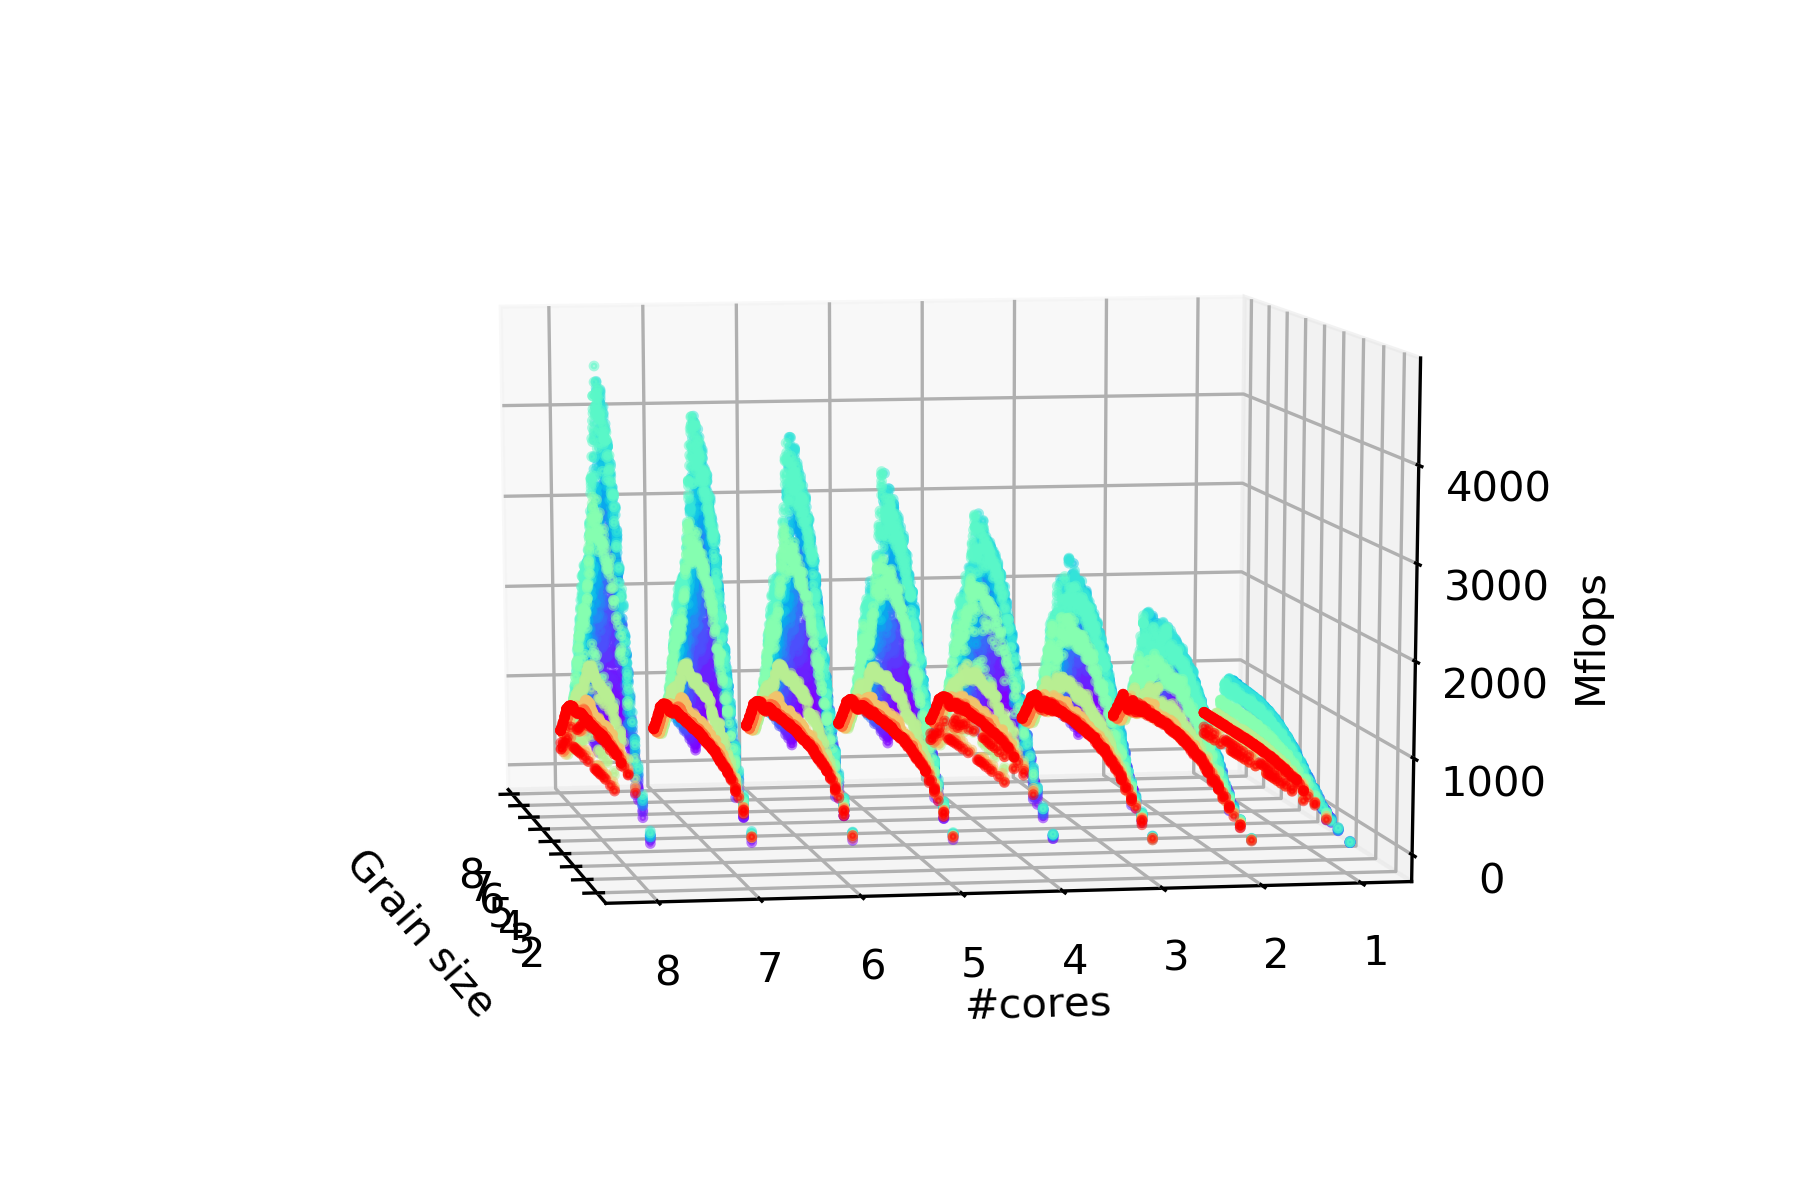
\includegraphics[width=1\linewidth]{images/fig4.png}
	\caption{The results obtained from running $DMATDMATADD$ benchmark through Blazemark for matrix sizes from 200$\times$200 to 1587$\times$1587}	
	\label{fig4}
\end{figure}

\vspace{\baselineskip}	
\subsection{Observation}
The final purpose of our experiments is to find a chunk size that gives us the best performance for a given matrix size on a given machine. This chunk size should also be tailored to the expression being executed, and this all is based on assuming that we have already fixed the block size.
So the first step appeared to be selecting the block size. For this purpose, we ran the experiments with a selection of block sizes as shown in Table~\ref{table1}.


It should be mentioned that there were three constraints on selecting the block sizes. First, Blaze forces the number of columns in a raw-major matrix to be divisible to SIMD register size in order to be able to take advantage of vectorization. Second, we have selected the number of columns in our blocks to be either divisible by cache line or to contain all the columns of the matrix.     


\begin{figure}[H]
	\centering
	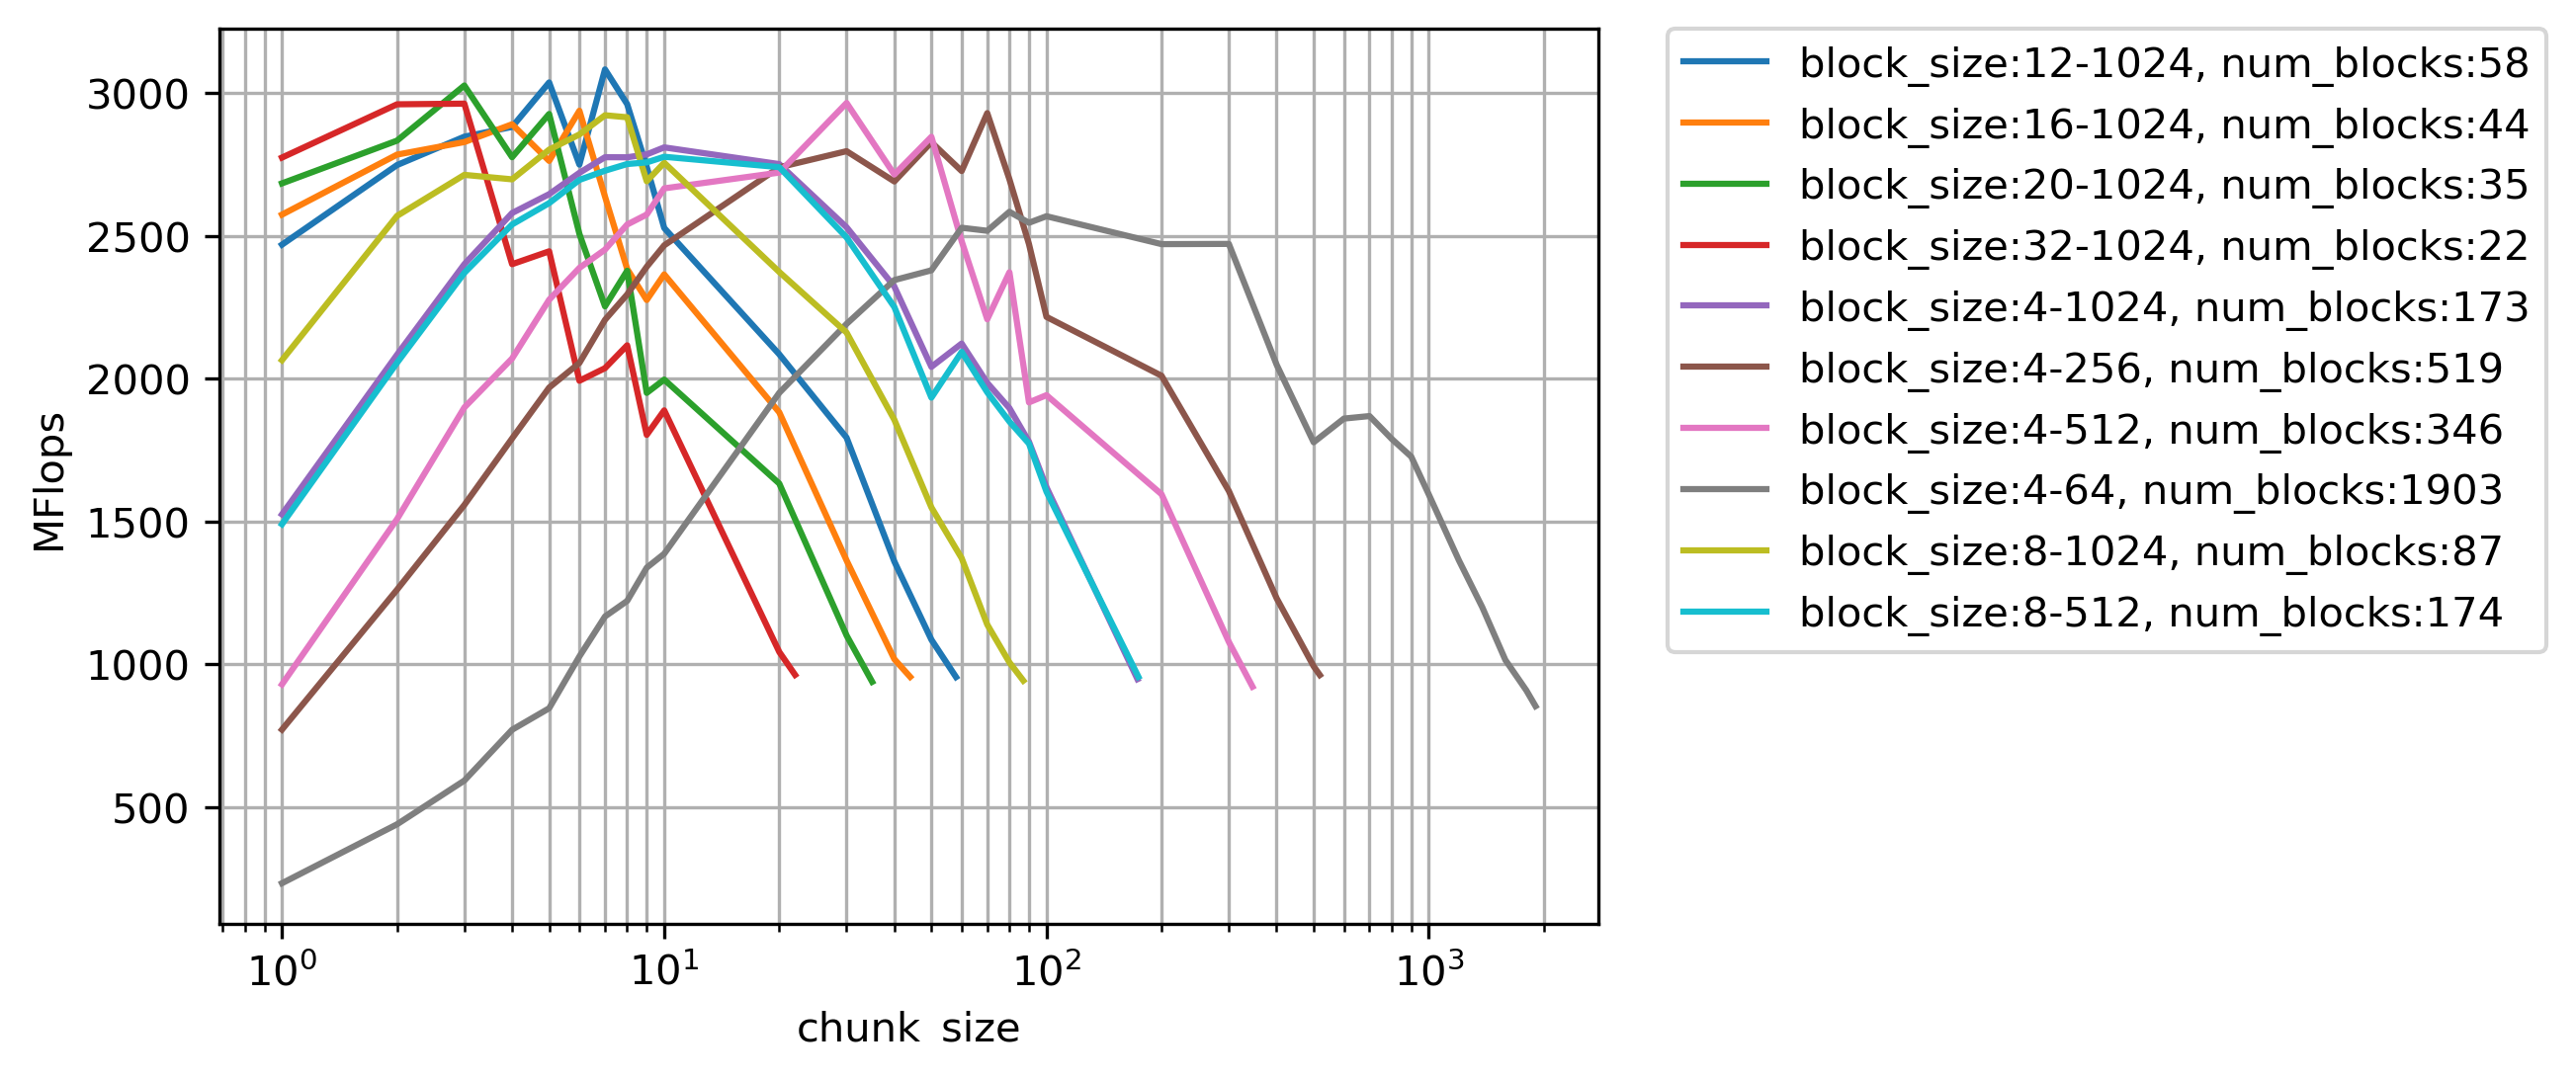
\includegraphics[width=1\linewidth]{images/fig5.png}
	\caption{The results obtained from running $DMATDMATADD$ benchmark through Blazemark for matrix sizes from 690$\times$690 with different combinations of block size and chunk size on $4$ cores}	
	\label{fig5}
\end{figure}

The collected data, as seen in Figure~\ref{fig5}, suggests two main points:
\begin{itemize}
	\item For each selected block size, there is a range of chunk sizes that gives us the best performance. 
	\item Except for some uncommon cases, no matter which block size we choose, we are able to achieve the maximum performance if we select the right chunk size.  
\end{itemize}

This motivated us to move our search parameter from chunk size to grain size. As stated earlier, grain size is the amount of work assigned to one HPX thread. Here we represent grain size by number of floating point operations performed by a HPX thread. For example, performing addition among two matrices, if we choose the block size as $4\times64$ and chunk size as $3$, the grain size would be $3\times4\times64=768$. 
Note that in our experiments whenever the number of columns of the original matrix is not divisible to the selected number of columns for block size, there would be a set of blocks with less number of elements than the selected block size, this has been considered when calculating the grain size.  

By changing our focus to the grain size instead of the block size and the chunk size, Figure~\ref{fig6} shows how the throughput changes with regards to the grain size for the $DMATDMATADD$ benchmark, for each specific block size. Each combination of block size and chunk size generates a point in the graph. On the other hand, Figure~\ref{fig9} looks at these graphs from another aspect, keeping the problem size constant but changing the number of the cores to run the benchmark on, instead.

\begin{figure}[H]
	\centering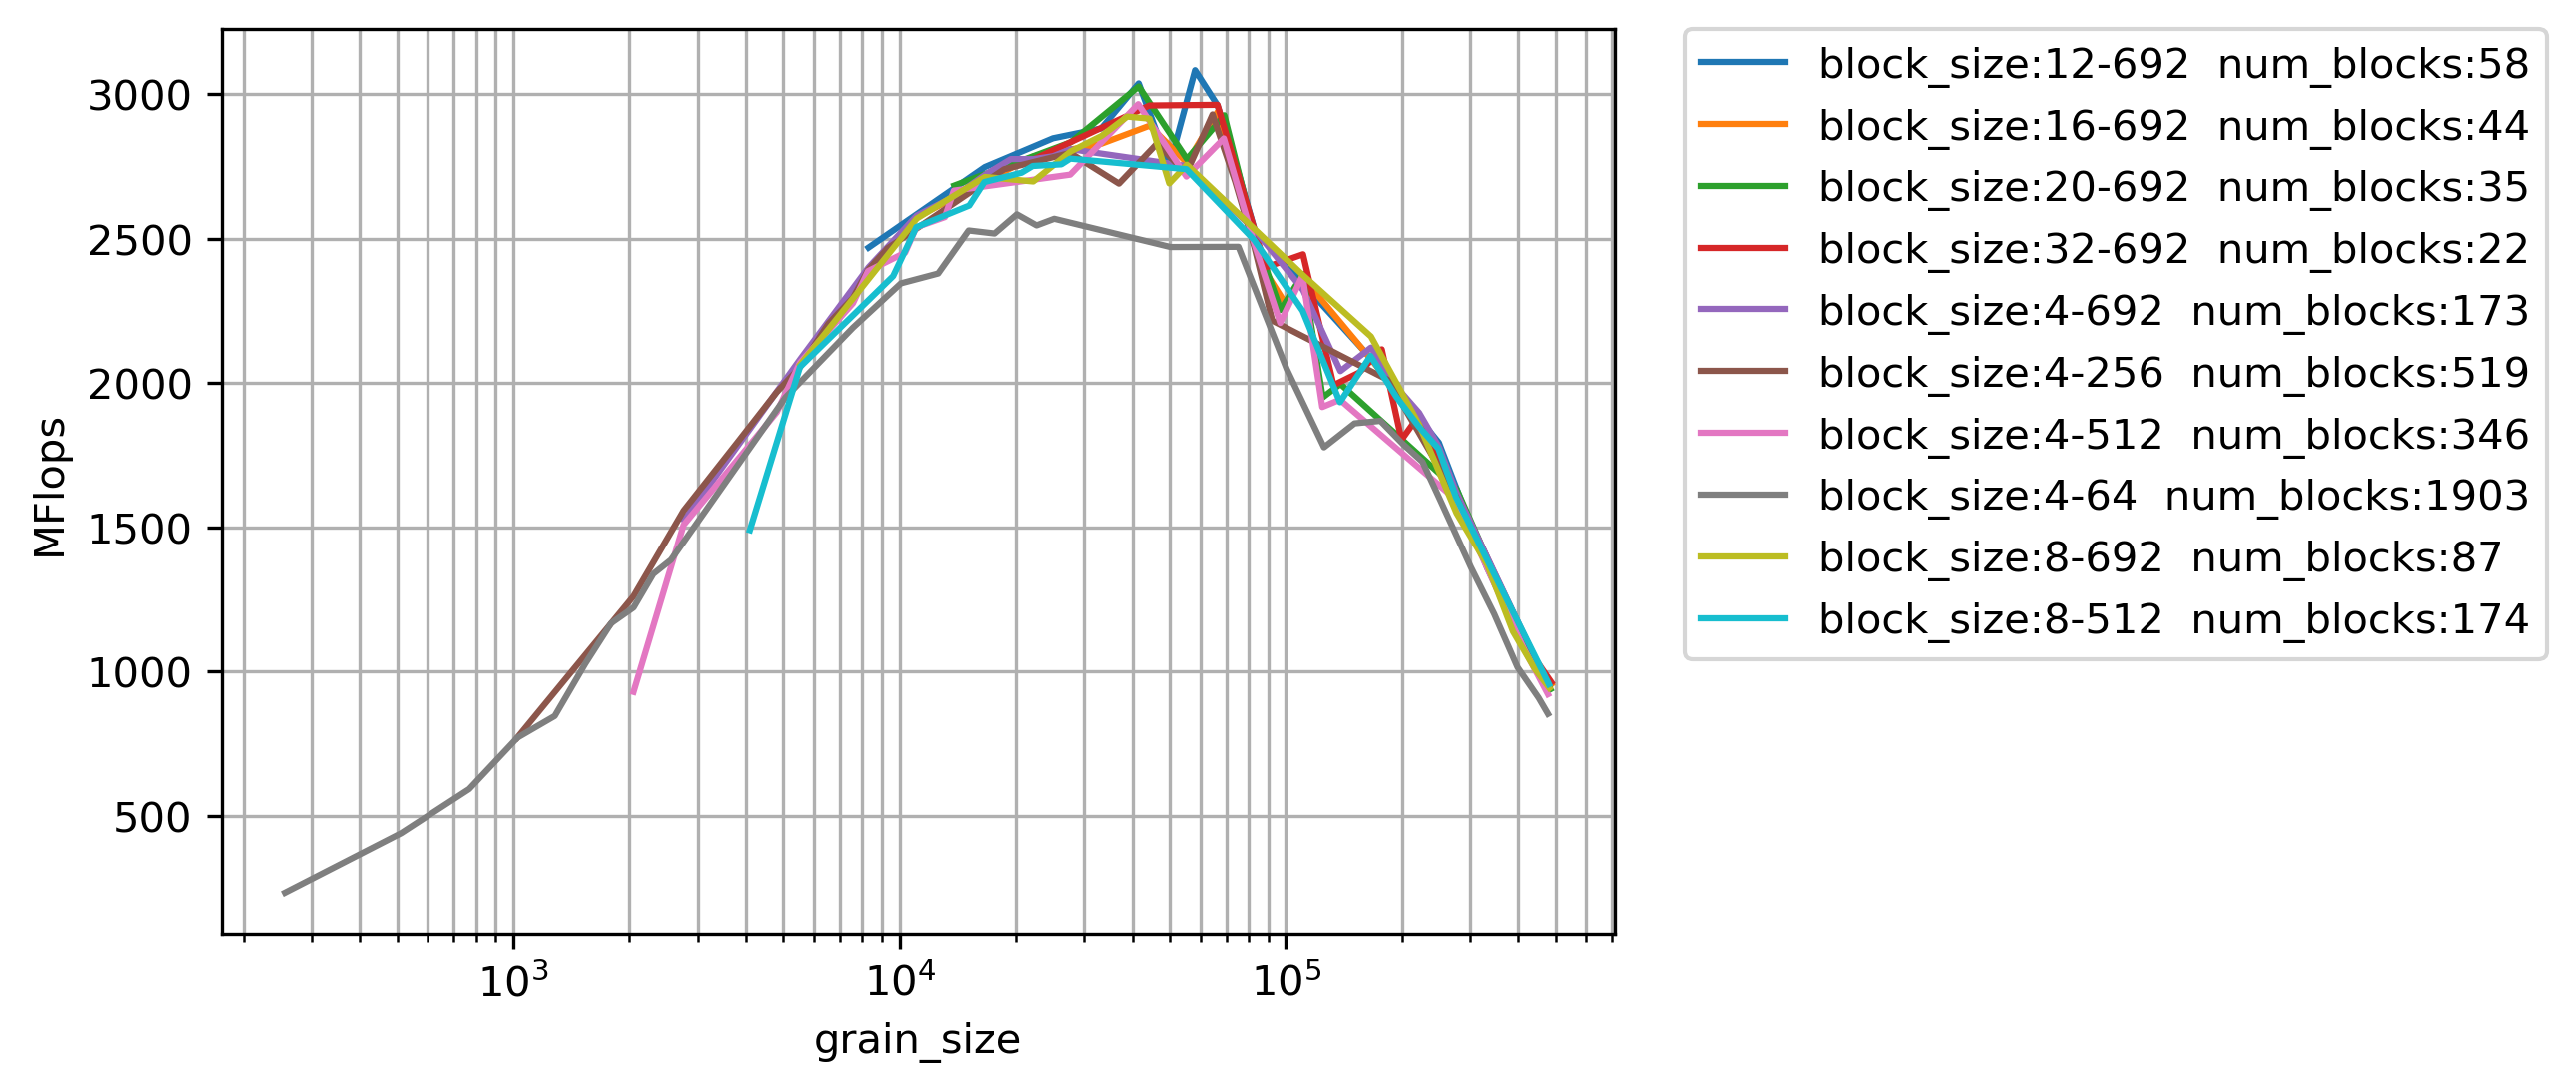
\includegraphics[width=1\linewidth]{images/fig6.png}
	\caption{The results obtained from running $DMATDMATADD$ benchmark through Blazemark for matrix size 690$\times$690 on $4$ cores}	
	\label{fig6}
\end{figure}

\begin{figure}[H]
	\centering
	\hspace*{-2cm}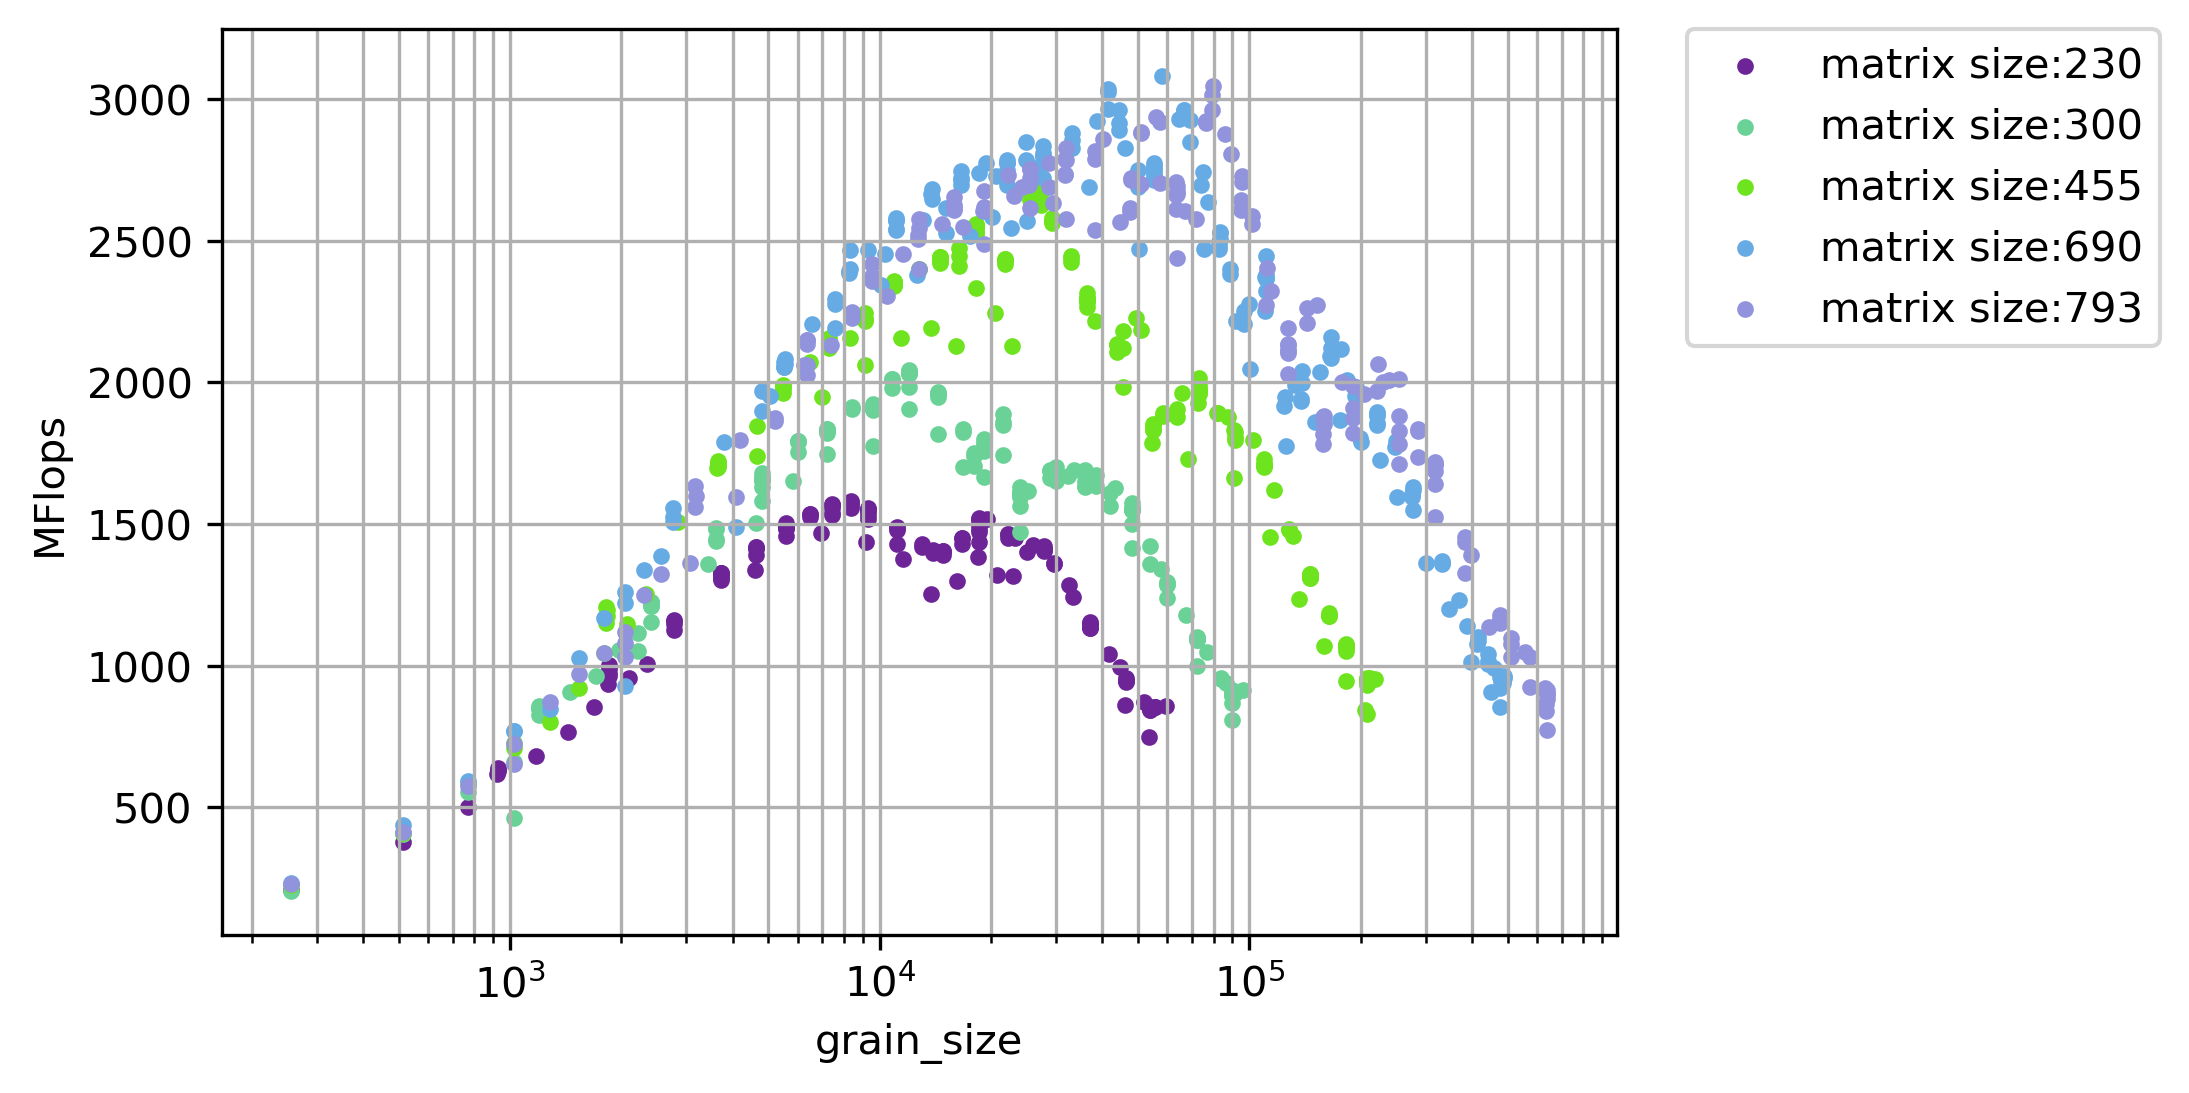
\includegraphics[scale=.75]{images/fig8.png}
	\caption{The results obtained from running $DMATDMATADD$ benchmark through Blazemark for 5 different matrix sizes on $4$ cores}	
	\label{fig7}
\end{figure}

\begin{figure}[H]
	\subfloat[]
	{\centering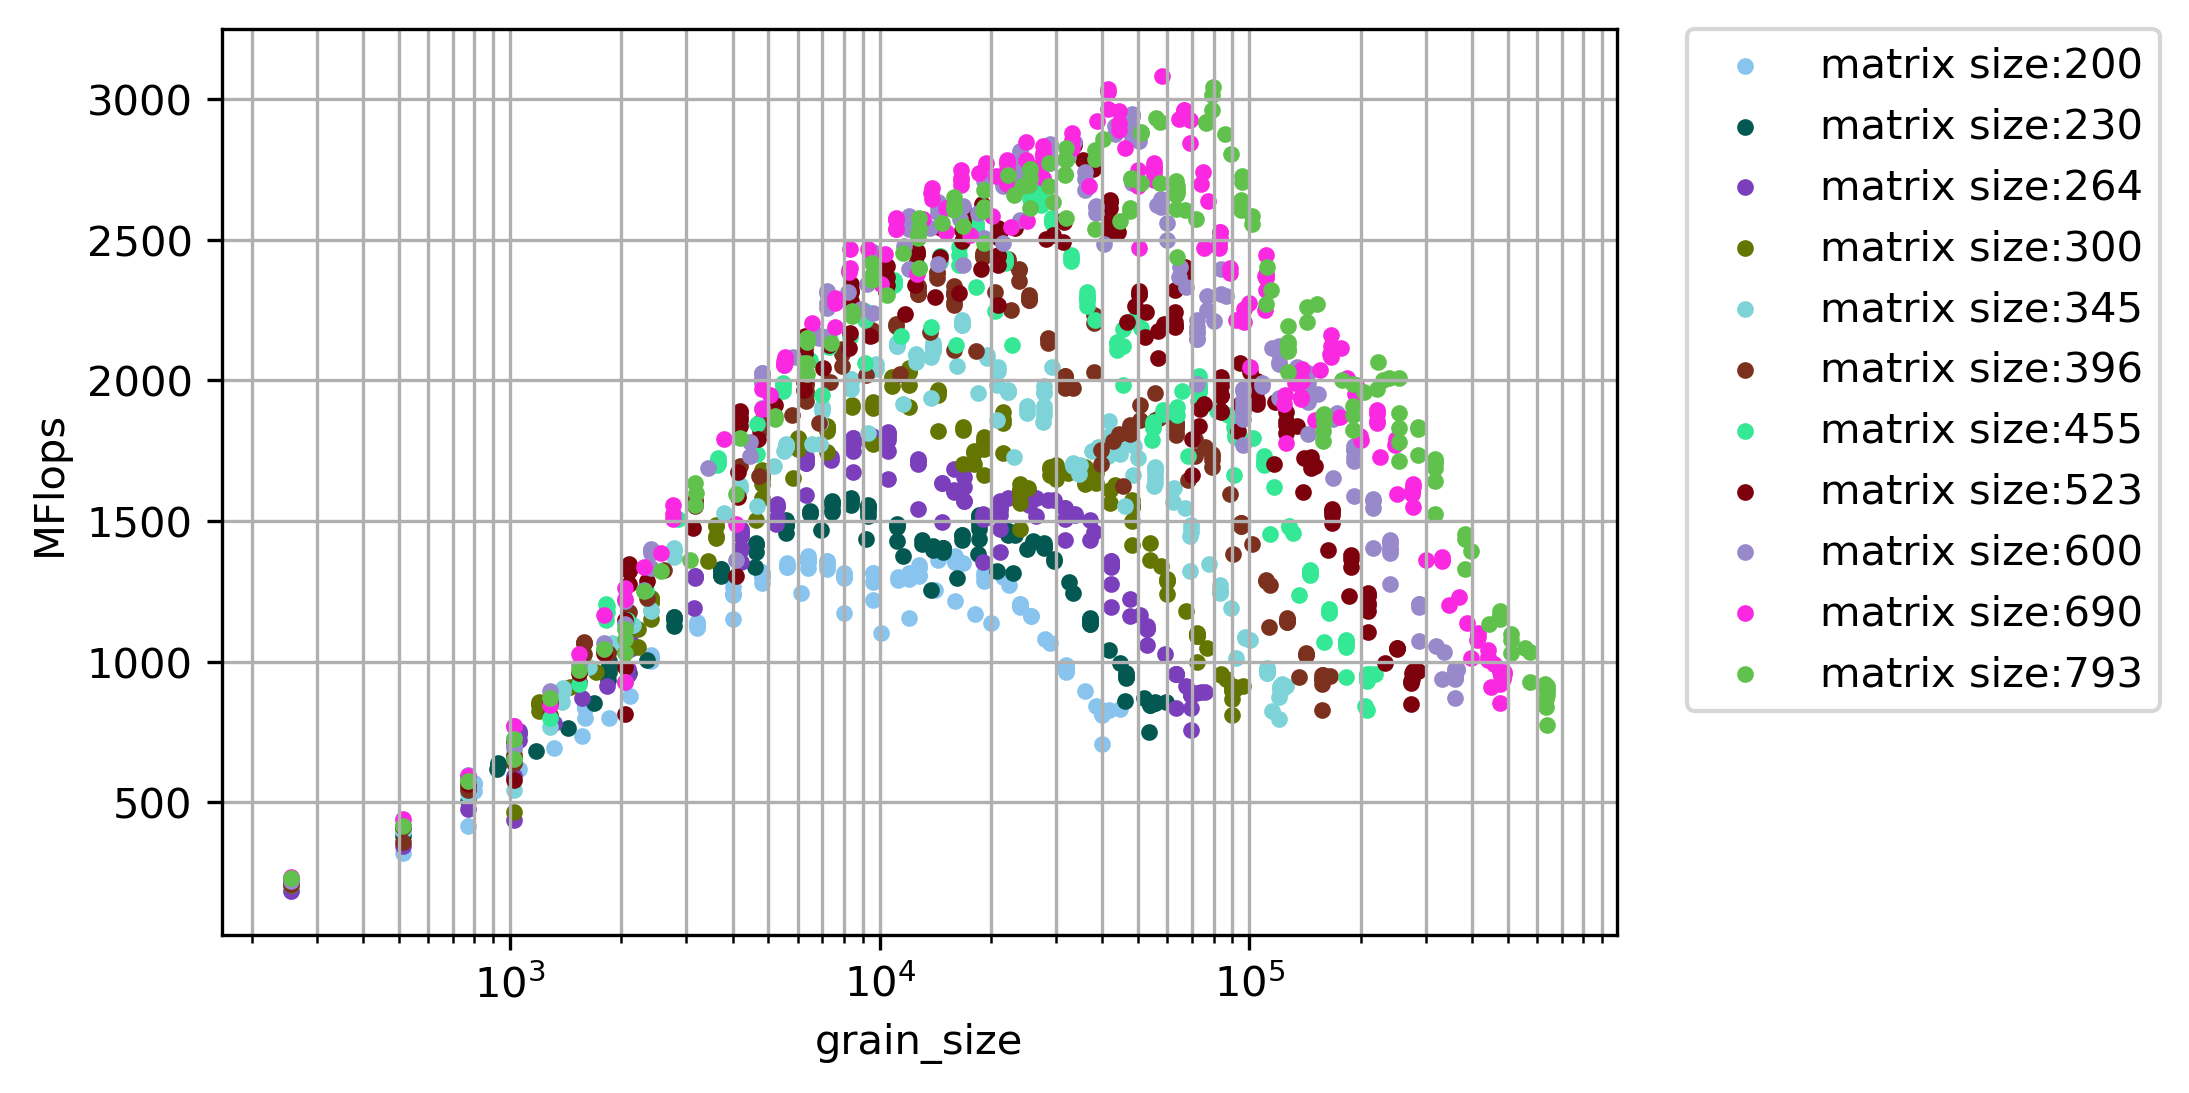
\includegraphics[scale=.75]{images/fig11.png}	
	\label{fig8:a}}

	\subfloat[]{
	\centering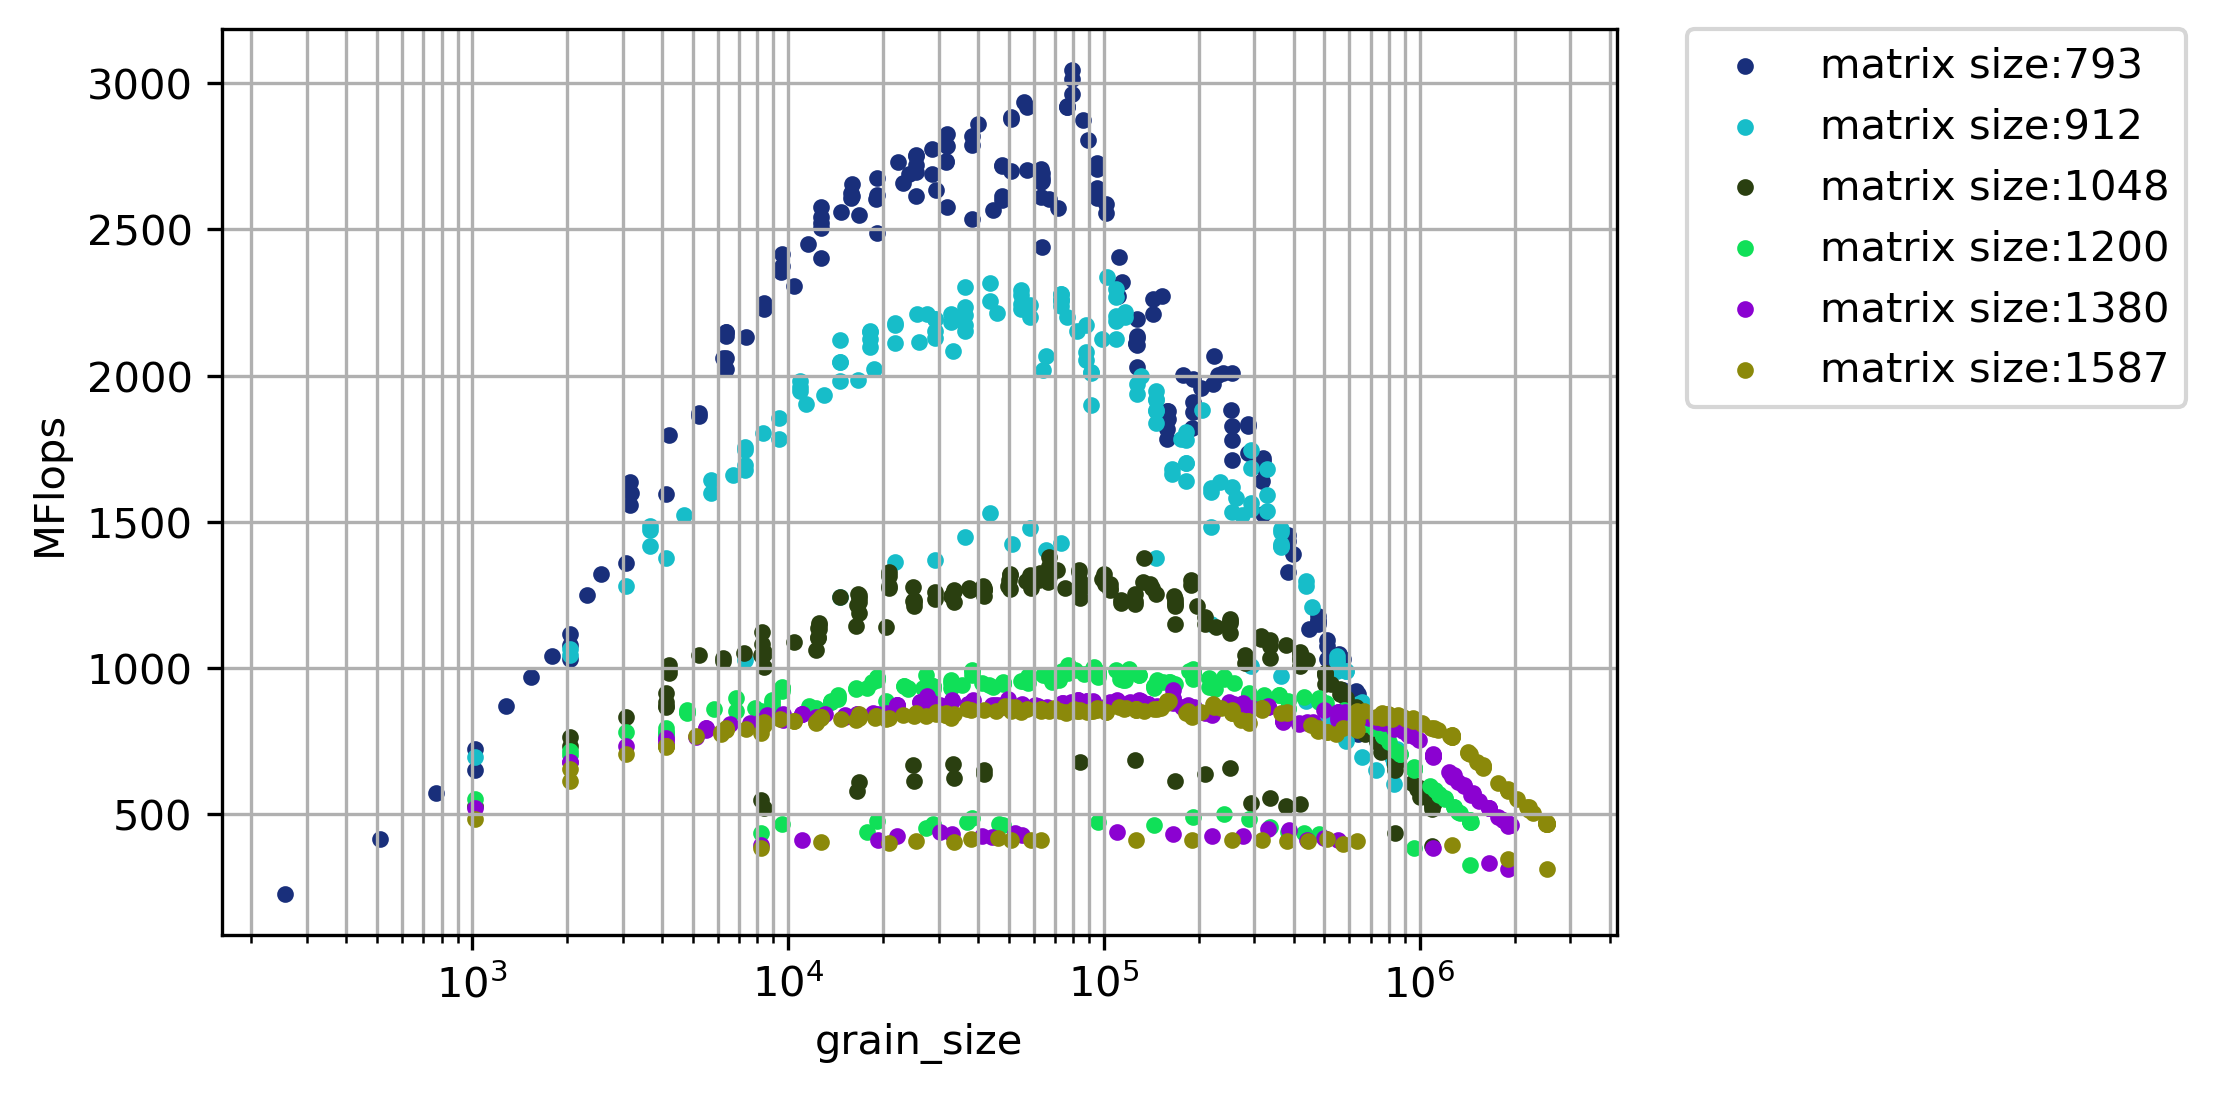
\includegraphics[scale=.75]{images/fig12.png}
	\label{fig8:b}}
	\caption{Throughput vs. grain size graph obtained from running $DMATDMATADD$ benchmark  on $4$ cores for matrix sizes (a) smaller than 793$\times$793 and (b) larger than 793$\times$793}
	\label{fig8}	
\end{figure}

\begin{figure}[H]
	\centering
	\hspace*{-2cm}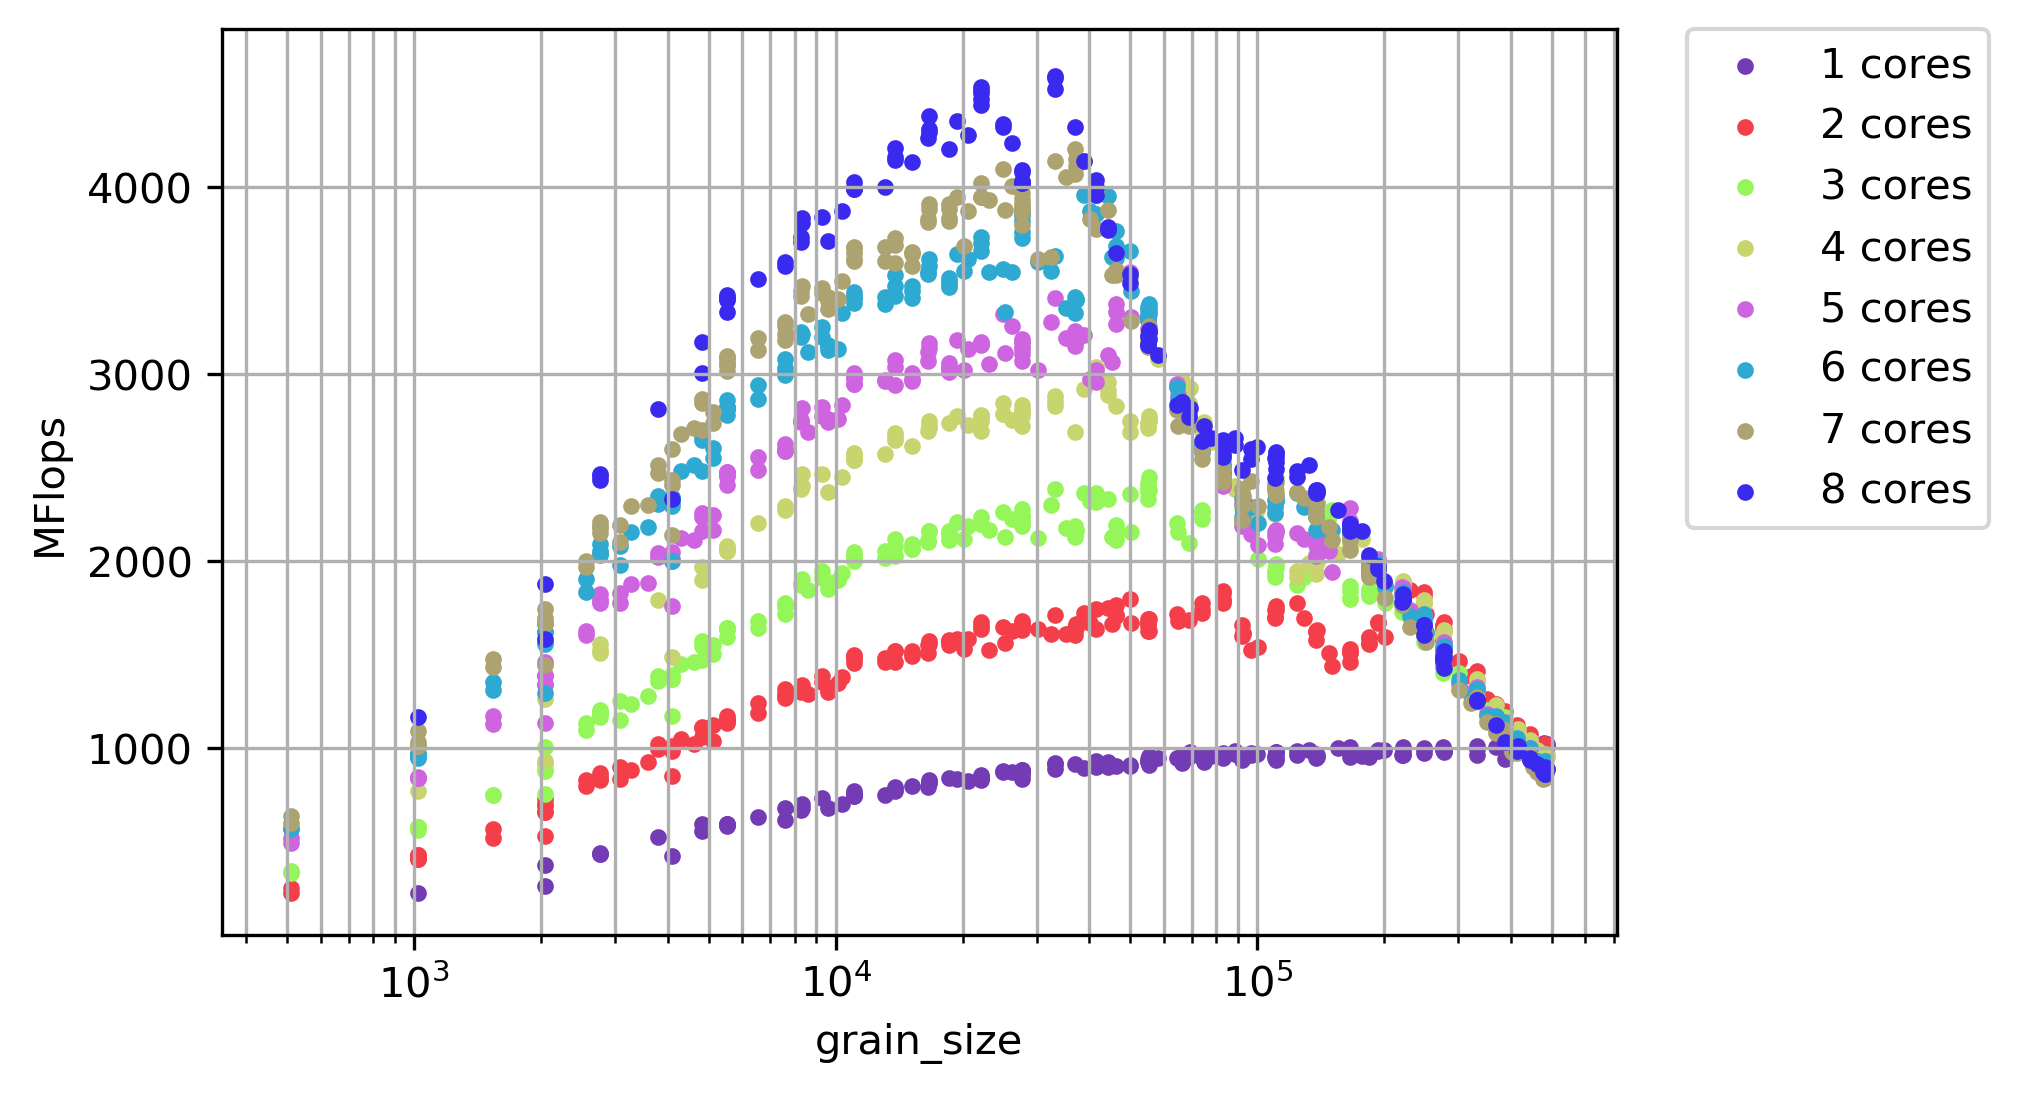
\includegraphics[scale=.75]{images/fig13.png}
	\caption{The results obtained from running $DMATDMATADD$ benchmark through Blazemark for matrix size 690$\times$690 on different number of cores}	
	\label{fig9}
\end{figure}

\vspace{\baselineskip}	
\section{Method}
Looking at the throughput vs. grain size graphs and the consistent pattern observable motivated us to try to model the relationship between throughput and grain size. 
In order to simplify the process and eliminate the effect of different possible factors, we started with limiting the problem to a fixed matrix size. 

\vspace{\baselineskip}	
\subsection{Polynomial Fit}
In our first attempt we used a 2nd degree polynomial to model throughput against grain size. For each matrix size, we fitted the corresponding graphs shown in Figure~\ref{fig8} to a second degree polynomial. 

\begin{figure}[H]
	\centering
	\subfloat[]{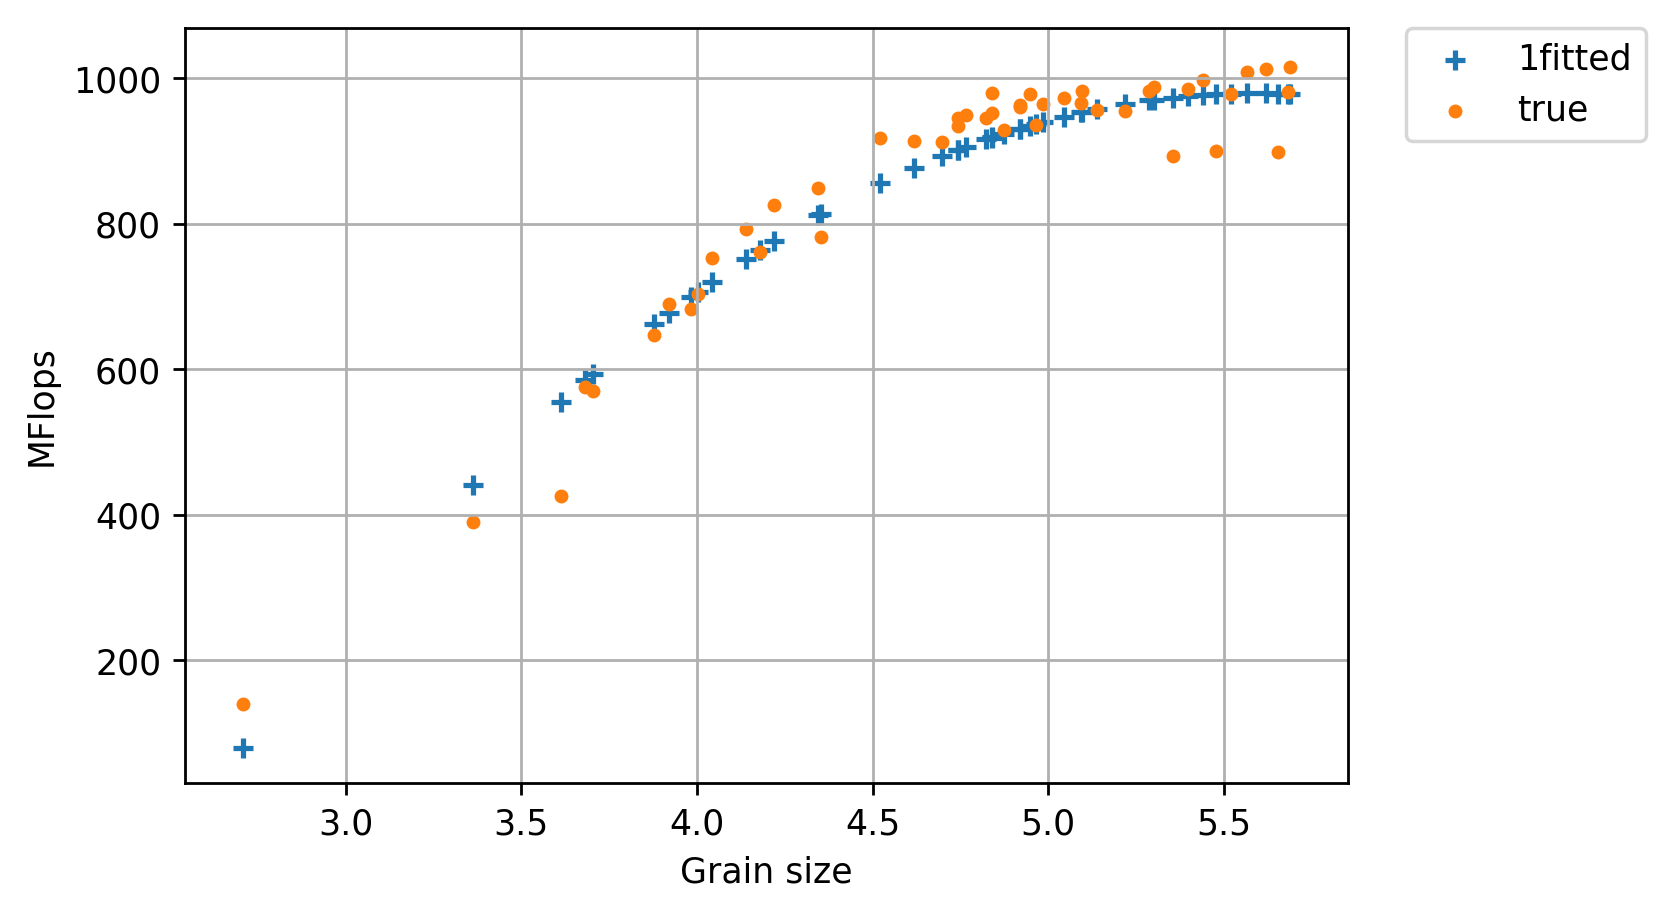
\includegraphics[scale=.45]{images/polyfit/fig_1_690.png}\label{fig10:a}}
	\subfloat[]{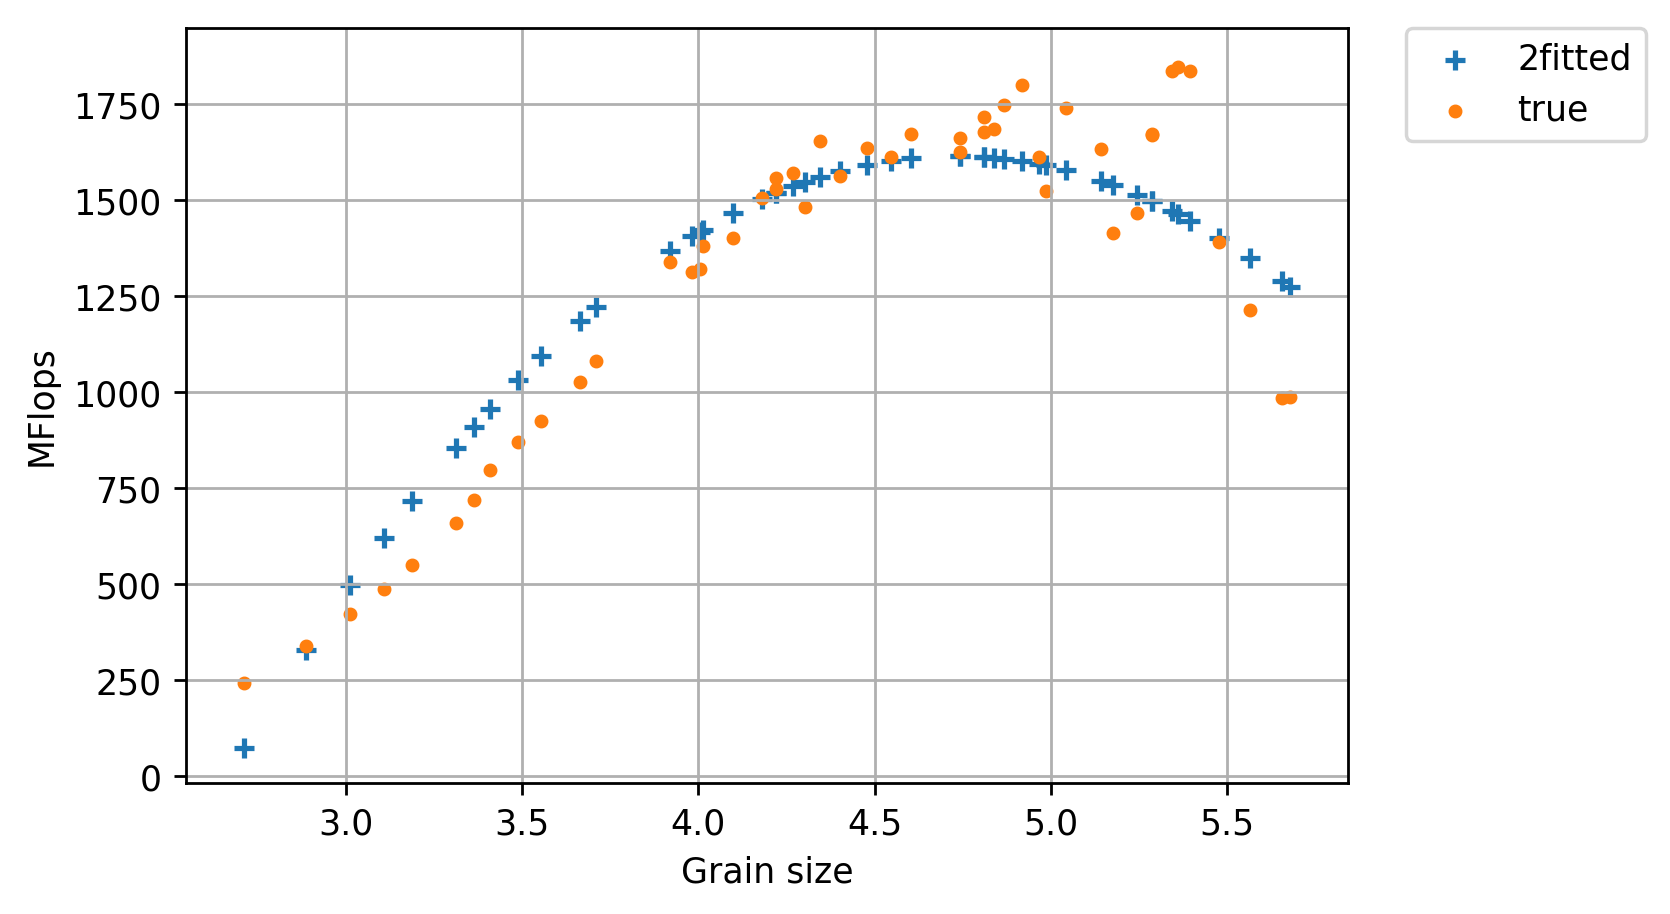
\includegraphics[scale=.45]{images/polyfit/fig_2_690.png}\label{fig10:b}}{\hfill}
	\subfloat[]{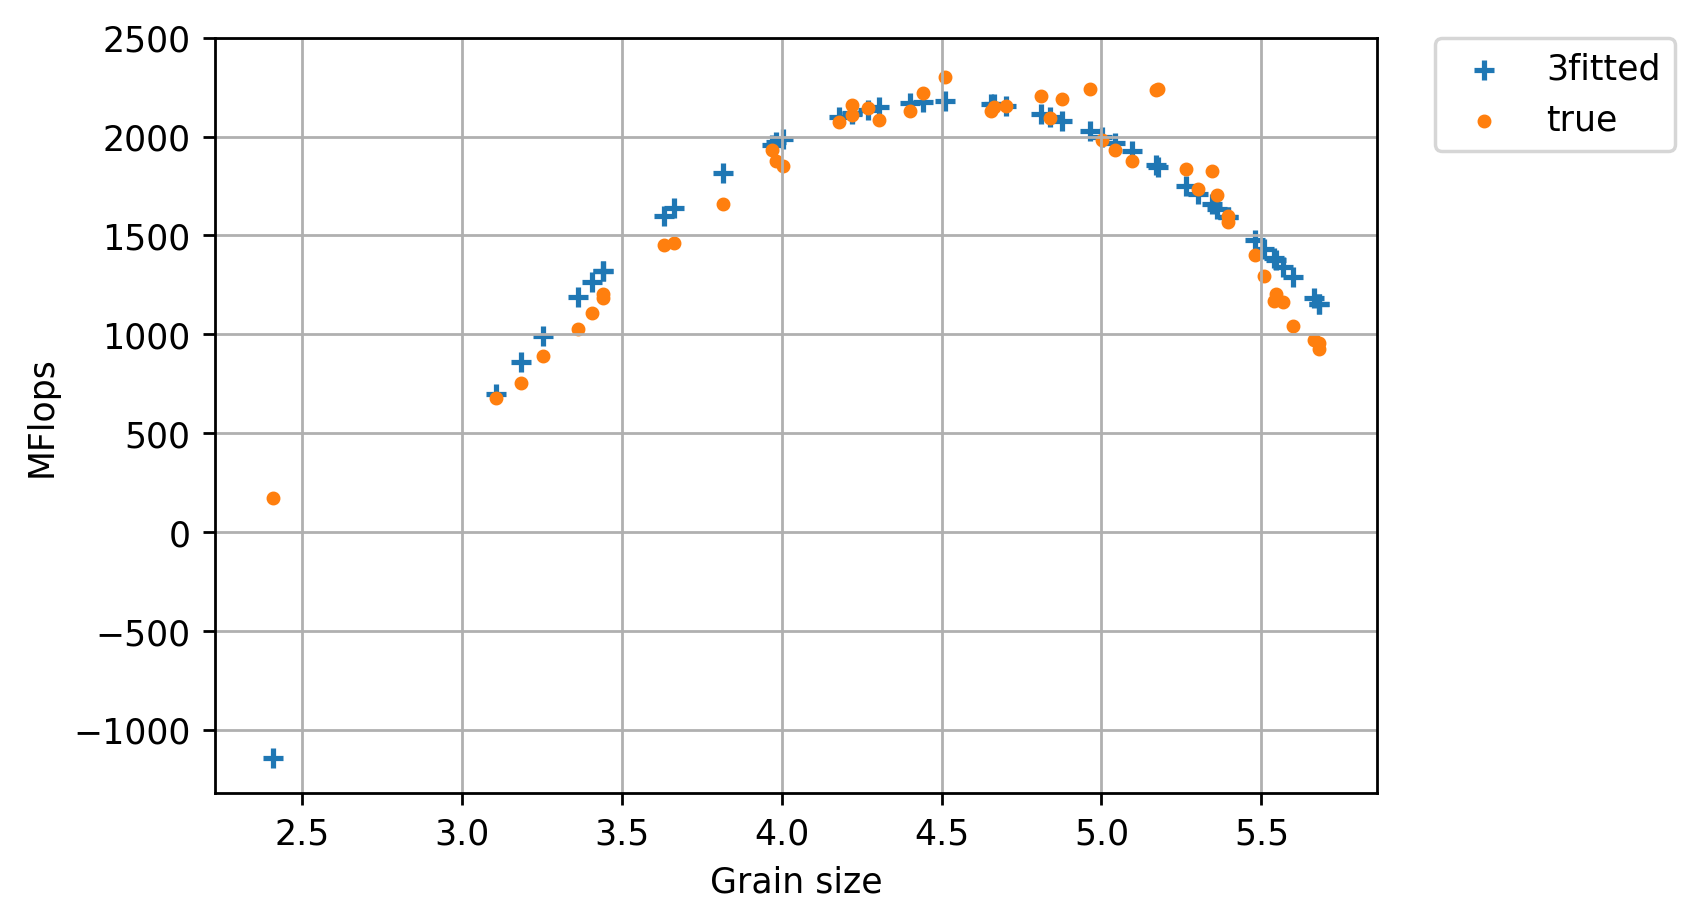
\includegraphics[scale=.45]{images/polyfit/fig_3_690.png}\label{fig10:c}}
	\subfloat[]{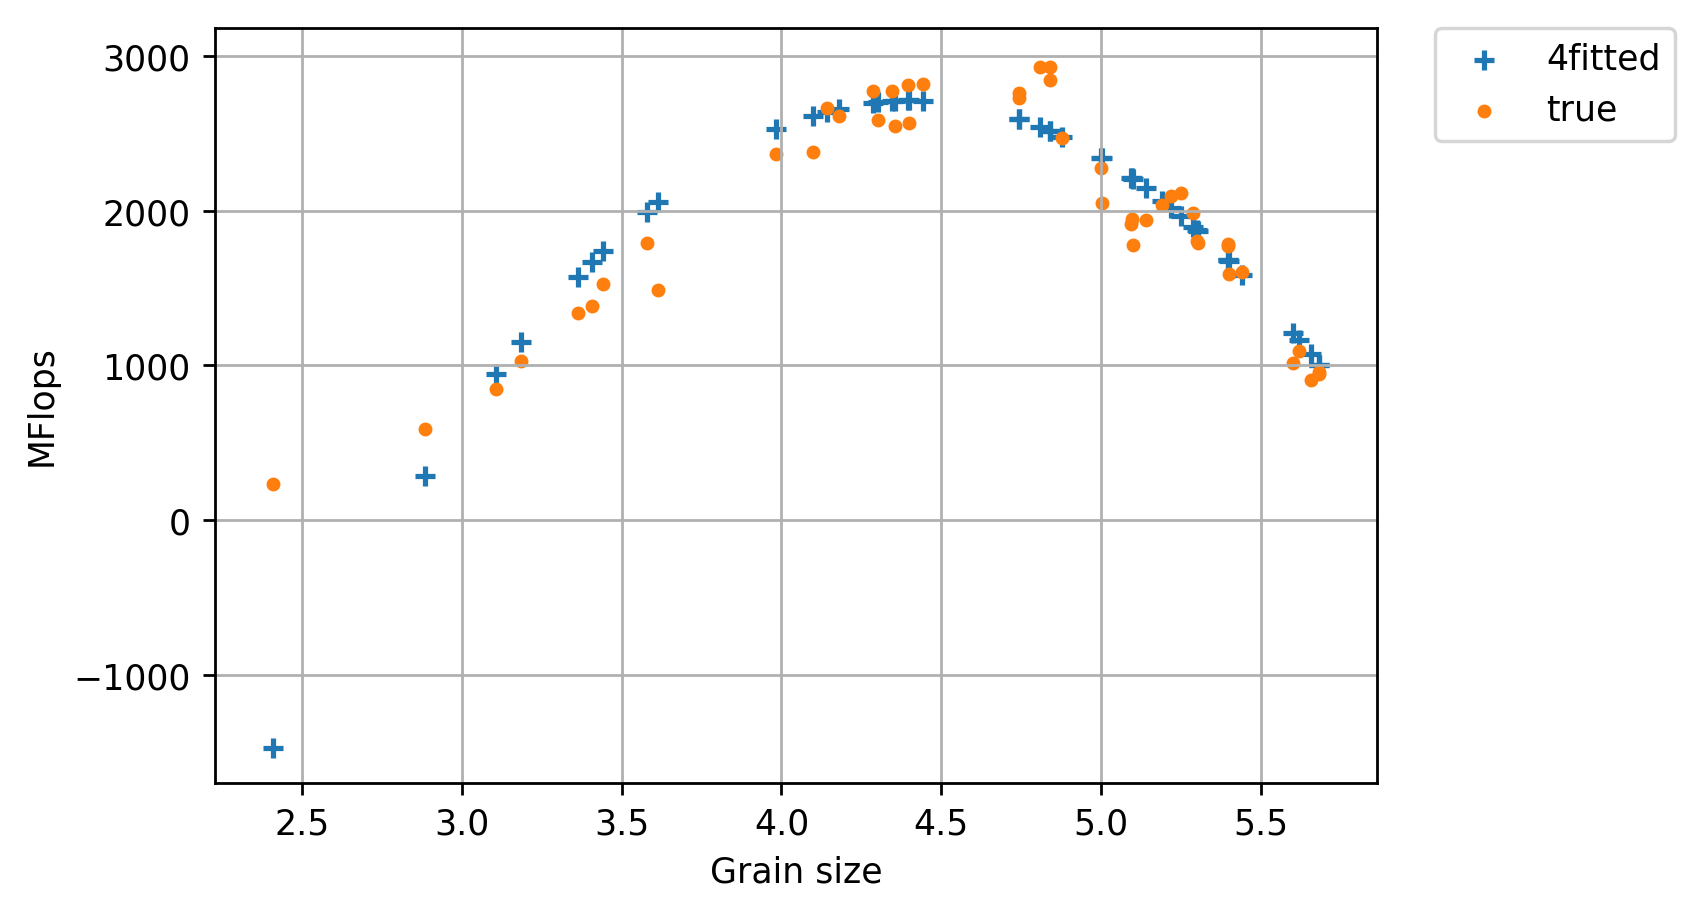
\includegraphics[scale=.45]{images/polyfit/fig_4_690.png}\label{fig10:d}}{\hfill}
	\subfloat[]{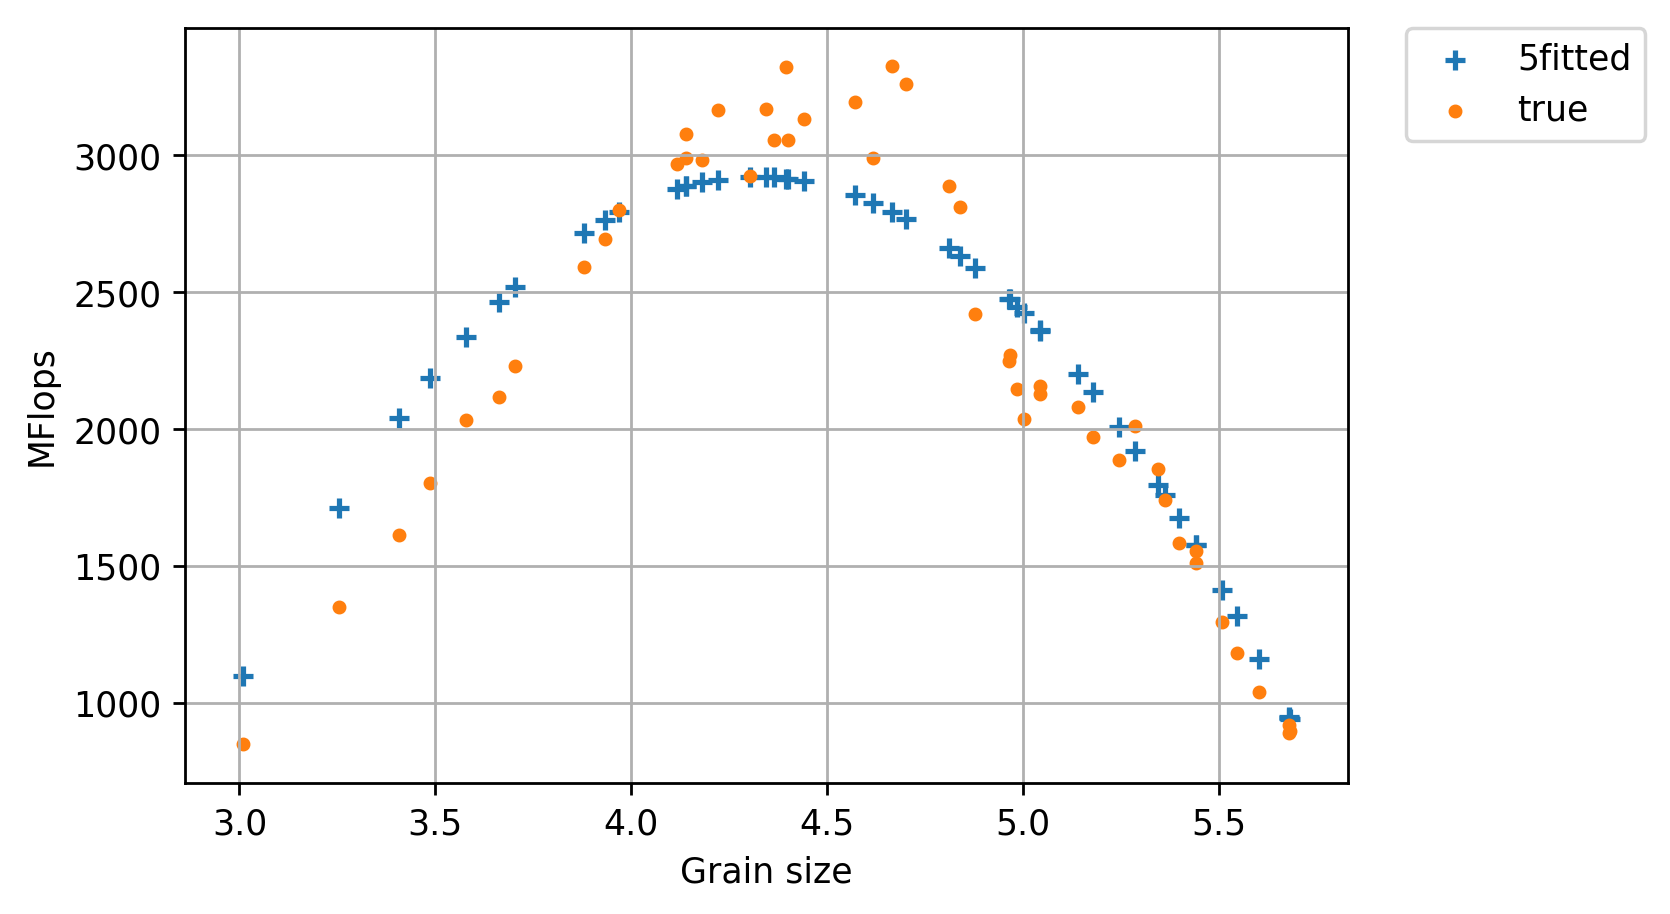
\includegraphics[scale=.45]{images/polyfit/fig_5_690.png}\label{fig10:e}}
	\subfloat[]{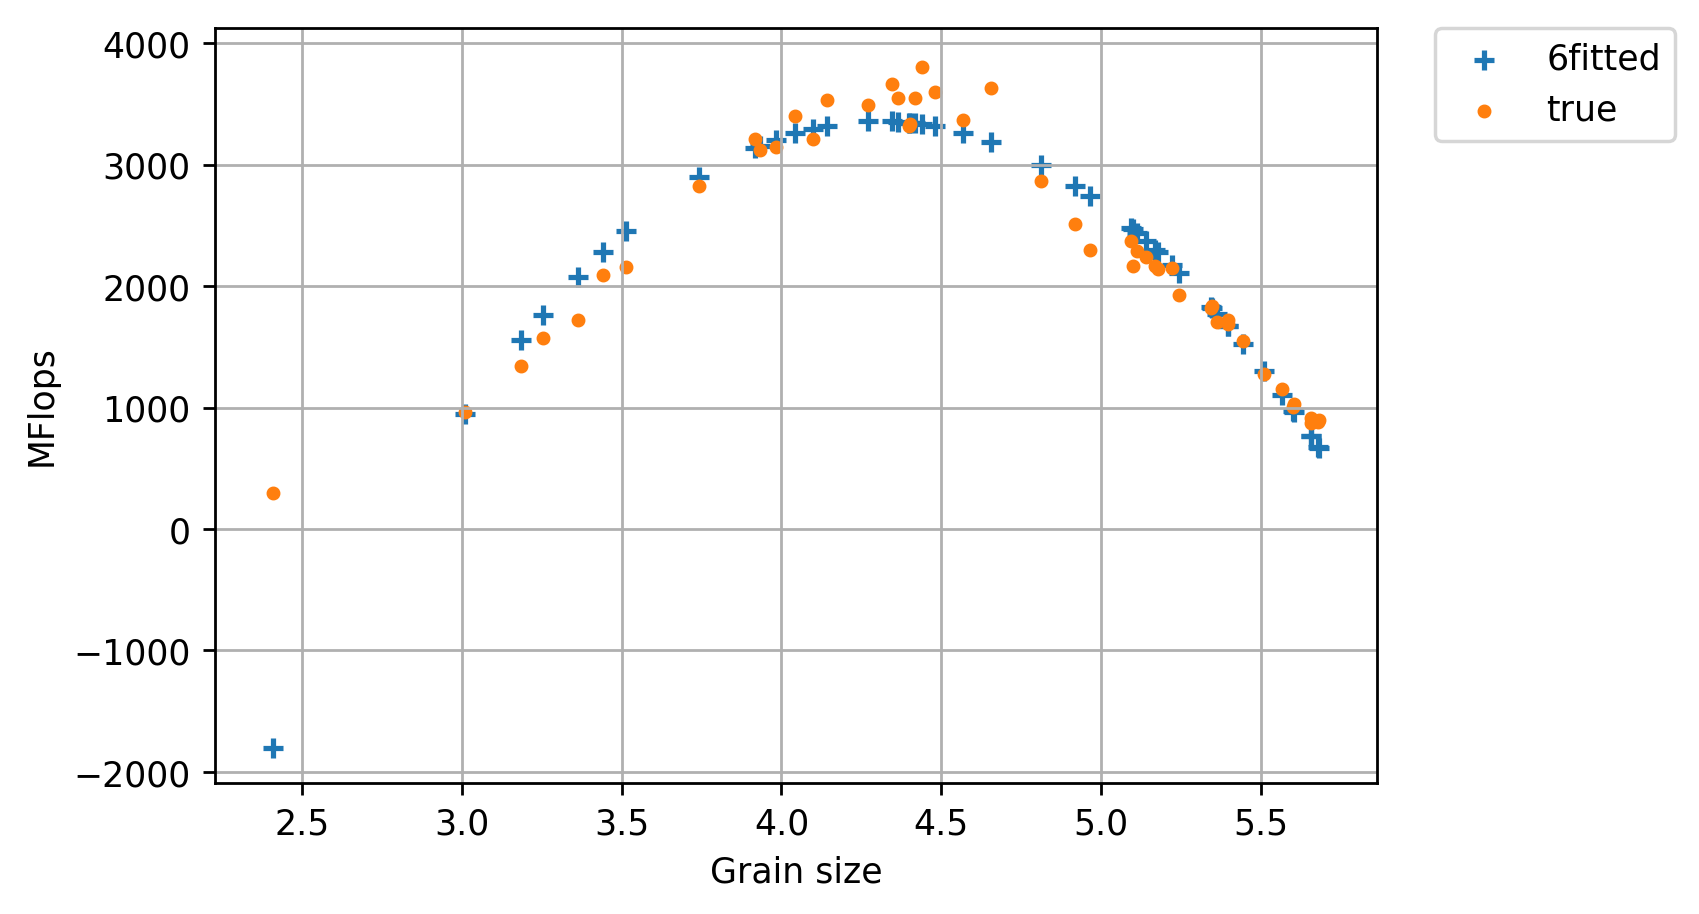
\includegraphics[scale=.45]{images/polyfit/fig_6_690.png}\label{fig10:f}}{\hfill}
	\subfloat[]{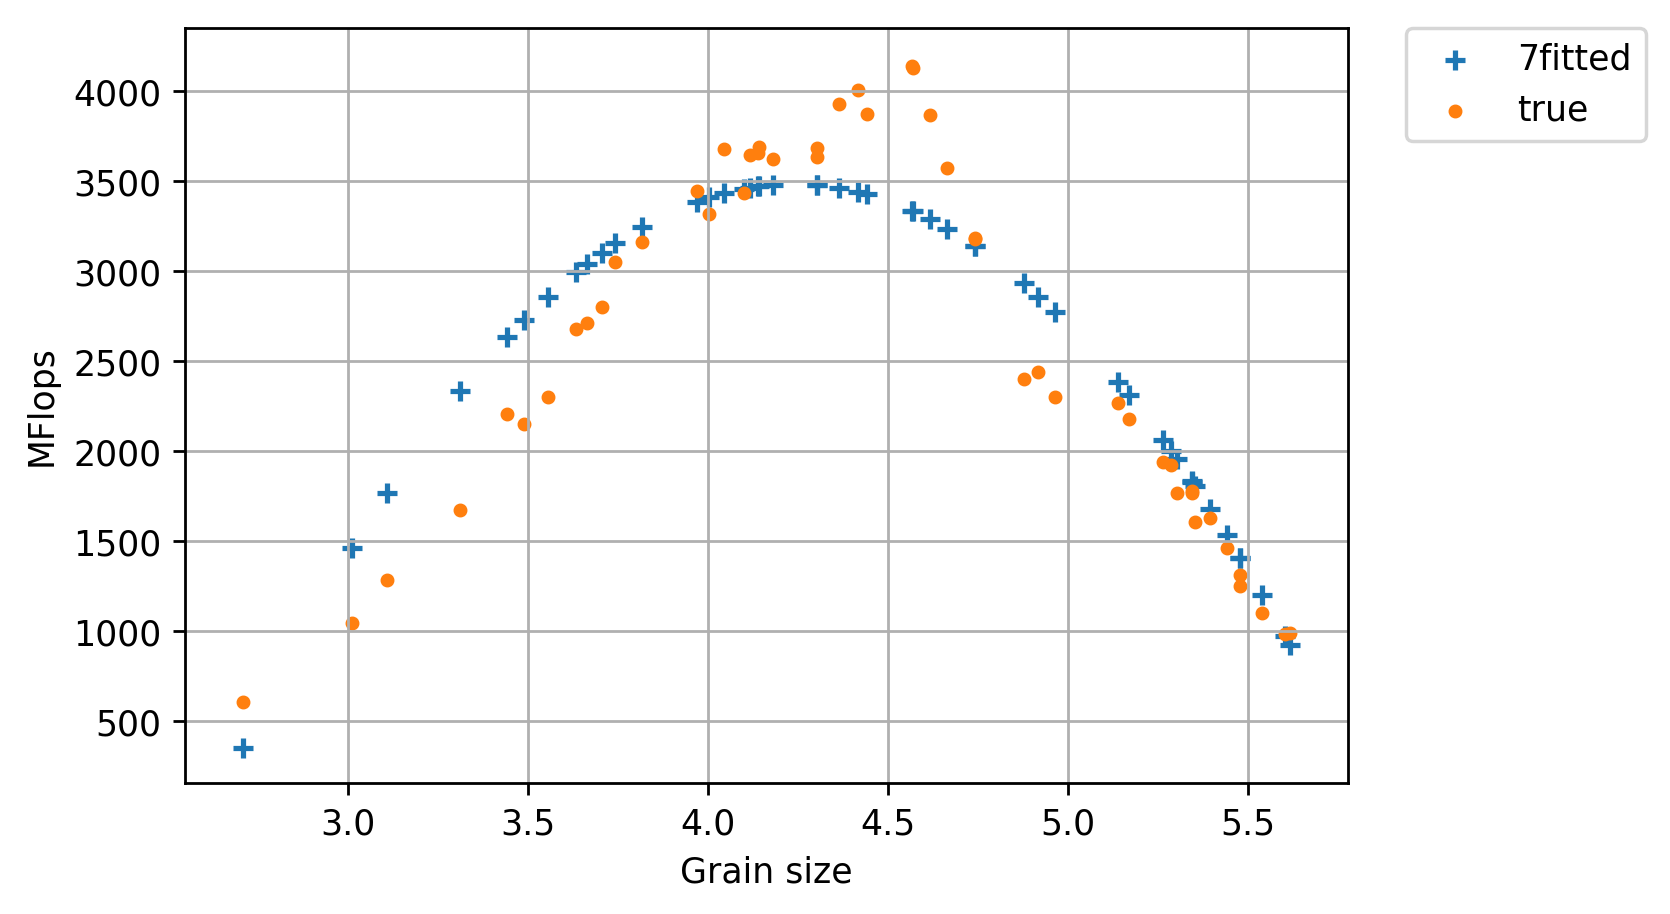
\includegraphics[scale=.45]{images/polyfit/fig_7_690.png}\label{fig10:g}}
	\subfloat[]{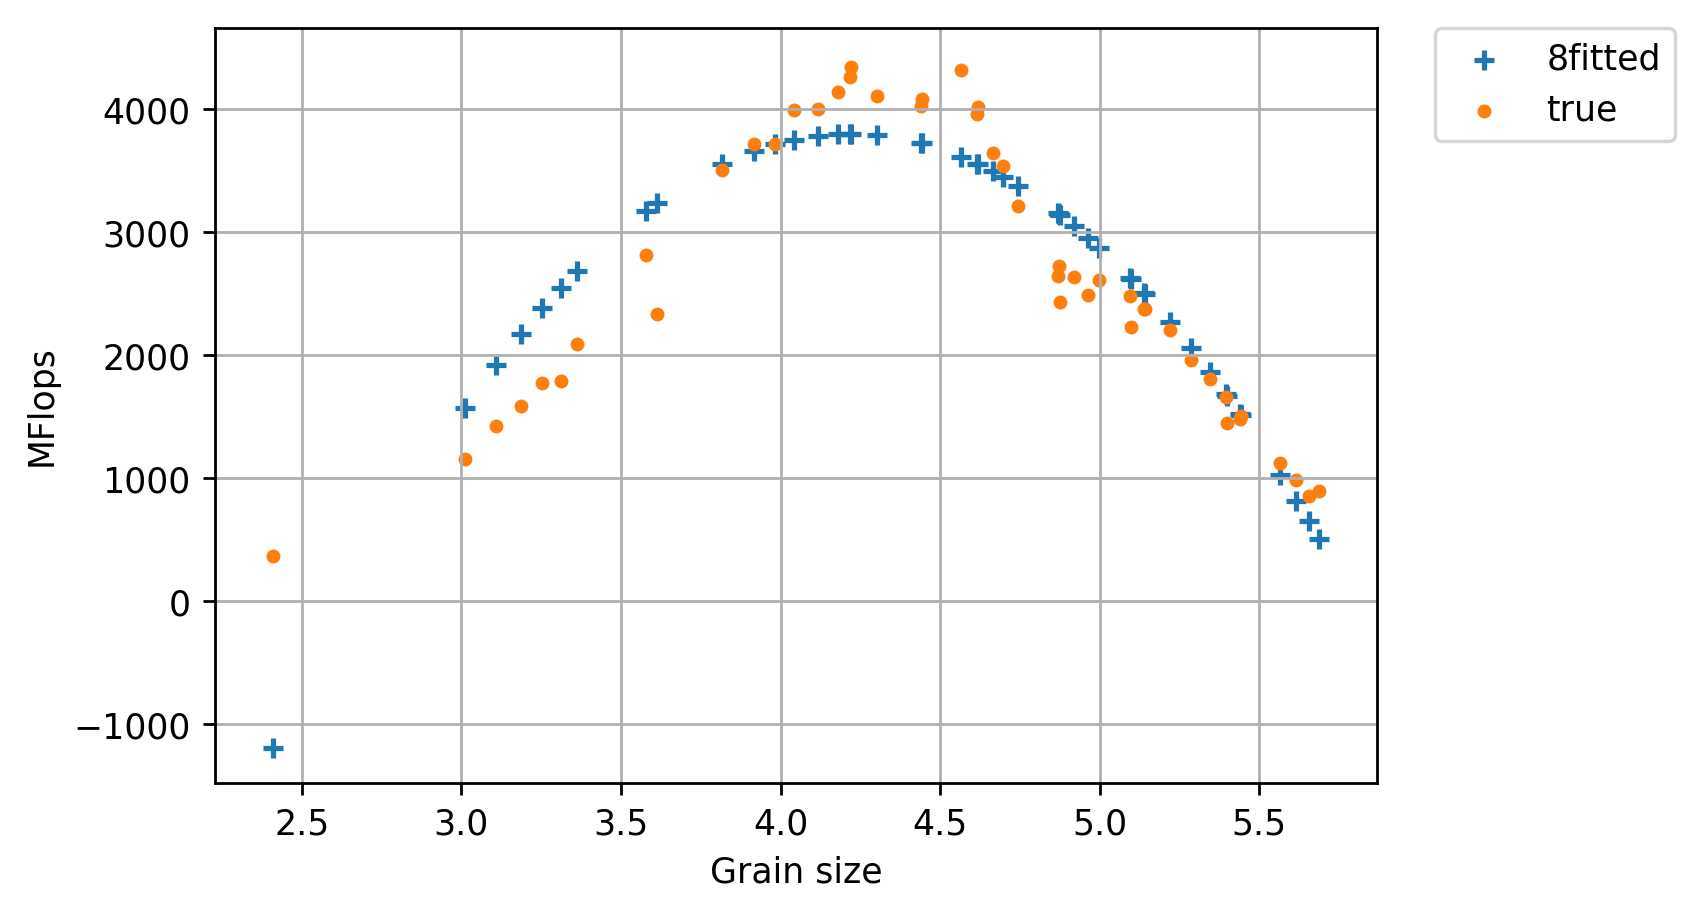
\includegraphics[scale=.45]{images/polyfit/fig_8_690.png}\label{fig10:h}}
							
	\caption{The results of fitting the throughput vs grain size data into a 2d polynomial for $DMATDMATADD$ benchmark for matrix size 690$\times$690 with different number of cores on the test data set (a) 1 core, (b) 2 cores, (c) 3 cores, (d) 4 cores, (e) 5 cores, (f) 6 cores, (g) 7 cores, (h) 8 cores}	
	\label{fig10}
\end{figure}


\vspace{\baselineskip}	
Figure~\ref{fig10} shows the results of using a quadratic function to fit the data for one matrix size with different number of threads. 

For our experiment, we divided the data into two sections, training and test. $60\%$ of the data was randomly chosen for the training part and the rest was considered as the test set. The training set was used to find the best 2nd degree polynomial for the data, and once the parameters were identified, the generated 2nd degree polynomial was applied to the test set to measure how good our fit was performing. 

For the matrix size $690\times690$ our dataset contained 117 data points, 72 of which was randomly selected to build the model. The mean relative error for each number of cores, calculated using Equation~\ref{eq2}, is represented in Figure~\ref{fig11} for training and test set. In this equation, $t_i$ and $p_i$ denote the true value and the predicted value of the $i$th sample respectively, where $n$ is the number of samples with the particular number of cores. 

\begin{equation}{\label{eq2}}
Relative Error = \frac{1}{n}\sum_{i=1}^{n} {1-p_i/t_i}
\end{equation}

\vspace{\baselineskip}	
\begin{figure}[H]
	\centering
	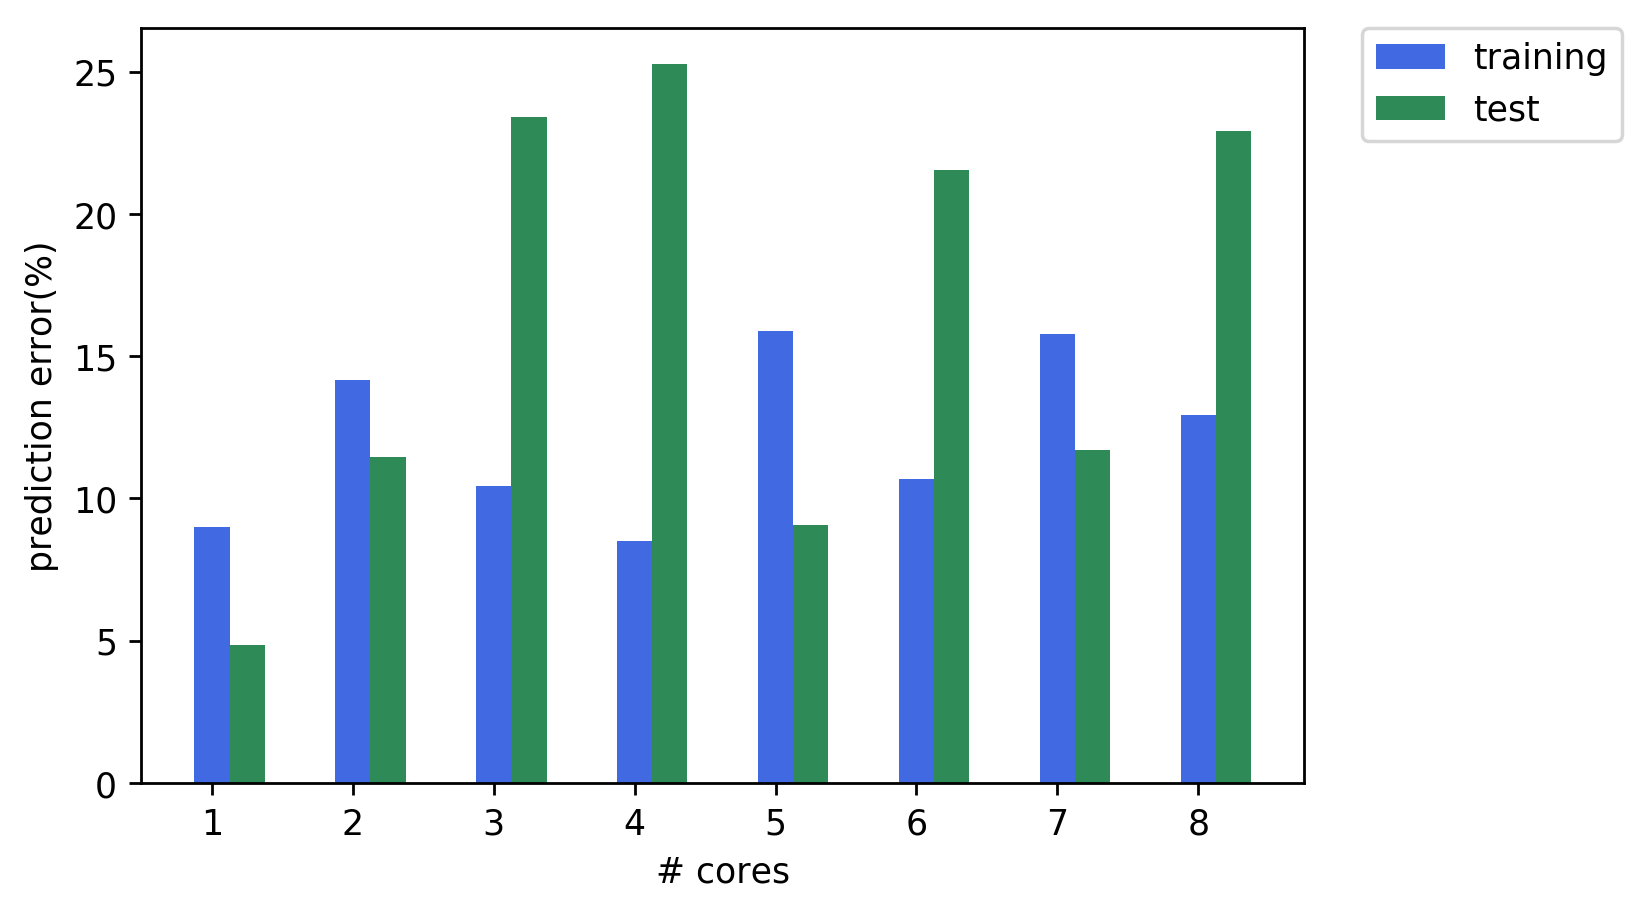
\includegraphics[scale=.75]{images/polyfit/fig_train_test_690.png}
	\caption{The training and test error for fitting data obtained from the $DMATDMATADD$ benchmark for matrix size $690\times690$ against different number of cores cores}	
	\label{fig11}
\end{figure}

\vspace{\baselineskip}	
\subsubsection{Generalizing the fitted function to include number of cores}
In this step, we try to generalize the fitted 2nd degree polynomial obtained from the previous step, represented by $P=ag^2+bg+c$, where $P$ is the throughput and $g$ is the grain size,by looking at how the three parameters $a$, $b$, and $c$ change when number of cores changes. 
A $3$rd degree polynomial seems to a reasonable fit for each of these parameters, in regards to number of cores. In order to avoid overfitting, we excluded two of the data points($2$ and $5$) from the data points used for fitting the polynomial and tested the fitted function on those two points to see how well the function is working on unseen data points. 


\vspace{\baselineskip}	
\begin{figure}[H]
	\centering
	\subfloat[]{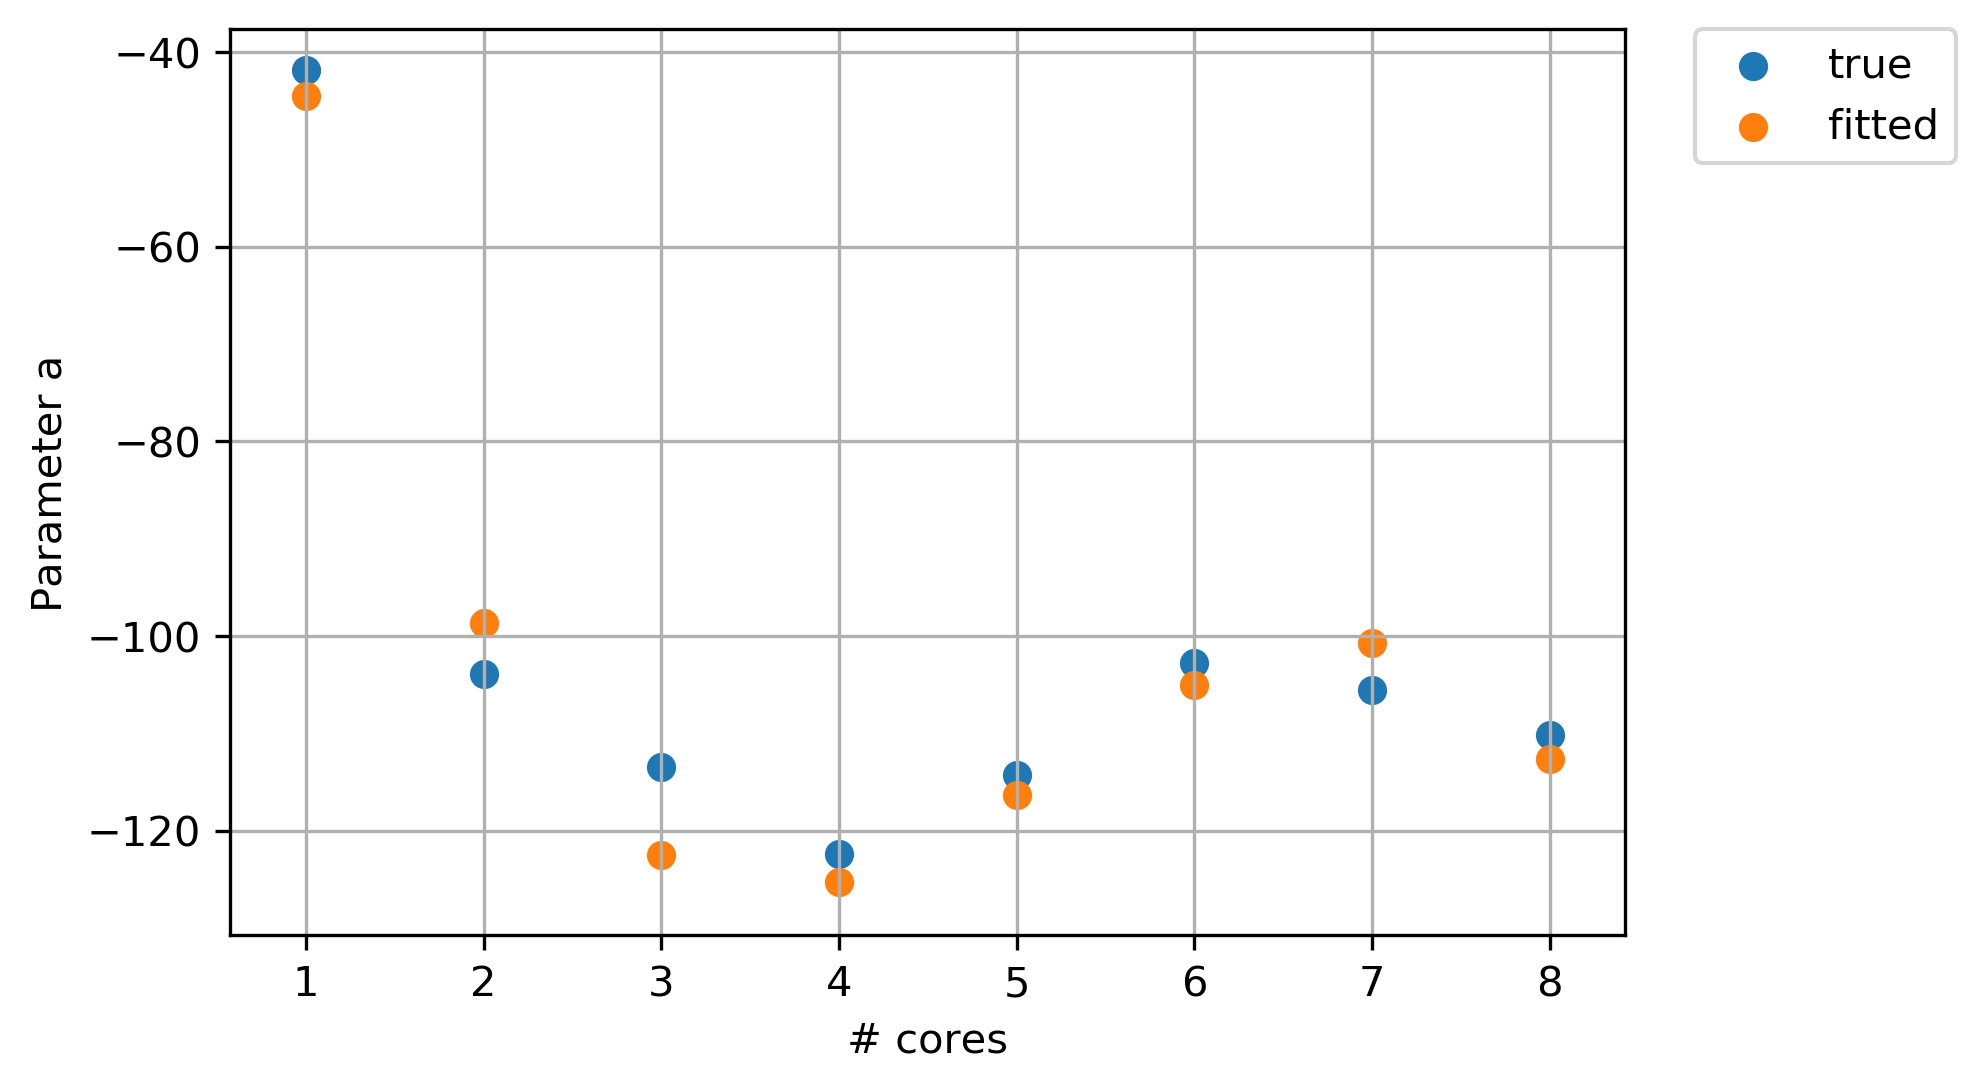
\includegraphics[scale=.3]{images/polyfit/fig_690_params_0.png}\label{fig15:a}}
	\subfloat[]{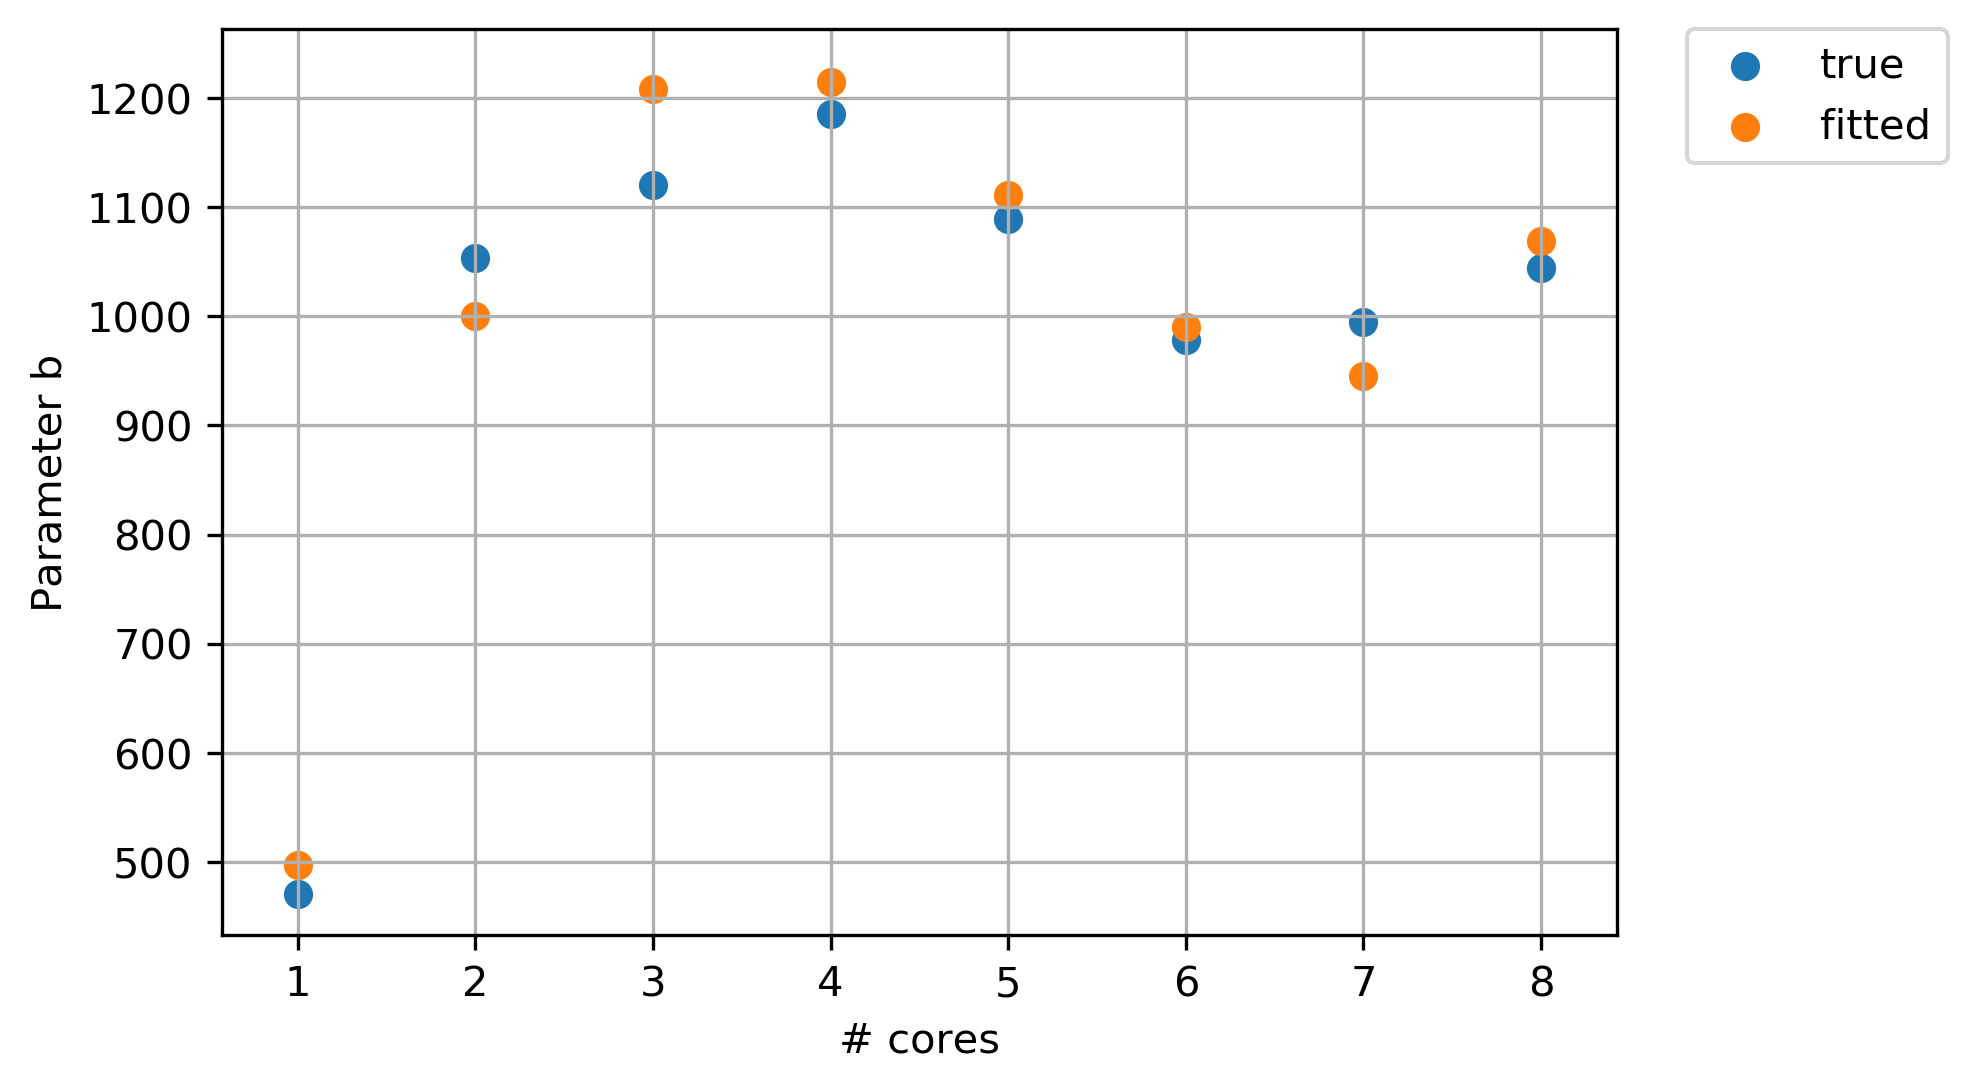
\includegraphics[scale=.3]{images/polyfit/fig_690_params_1.png}\label{fig15:b}}
	\subfloat[]{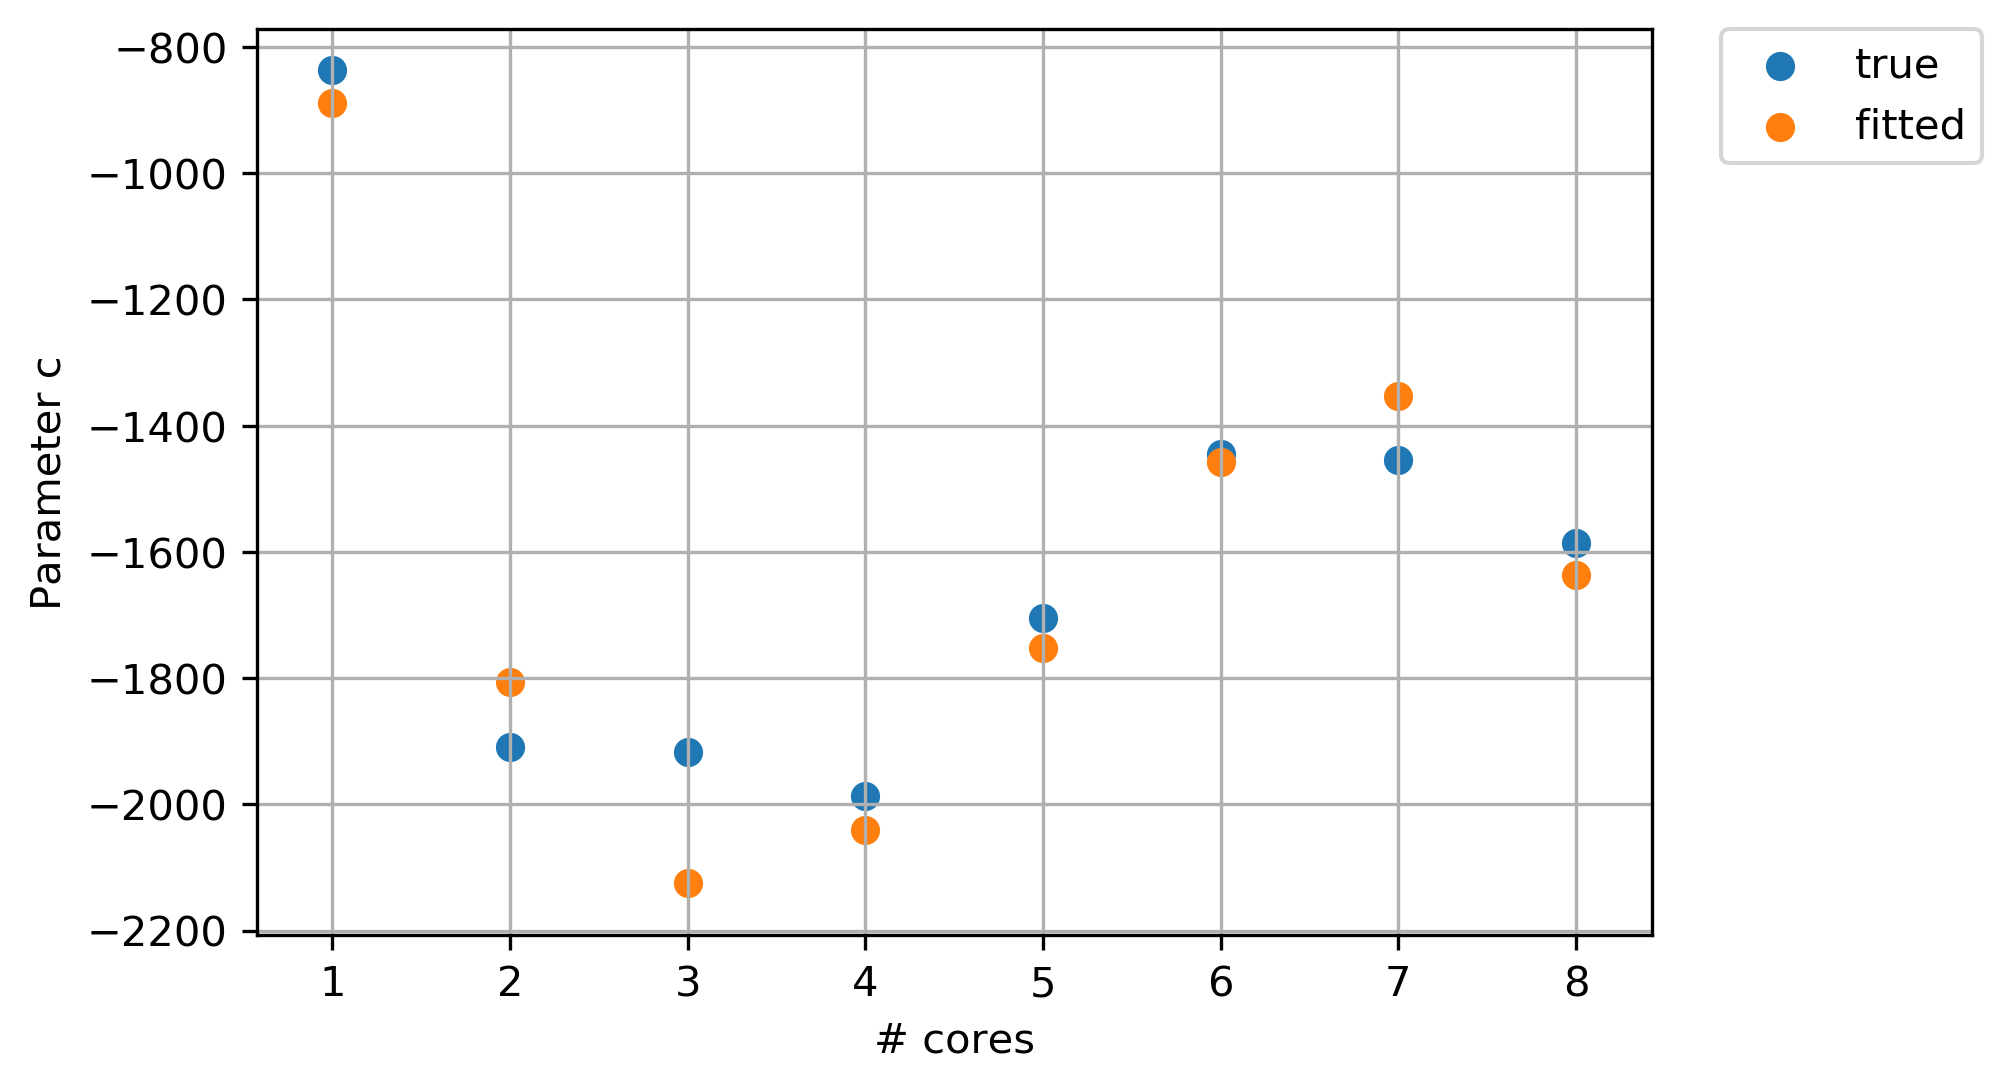
\includegraphics[scale=.3]{images/polyfit/fig_690_params_2.png}\label{fig15:c}}
	\caption{Fitting the parameters of the quadratic function with a $3$rd degree polynomial from the $DMATDMATADD$ benchmark for matrix size $690\times690$ against different number of cores.}	
	\label{fig15}
\end{figure}

\vspace{\baselineskip}	
\begin{figure}[H]
	\centering
	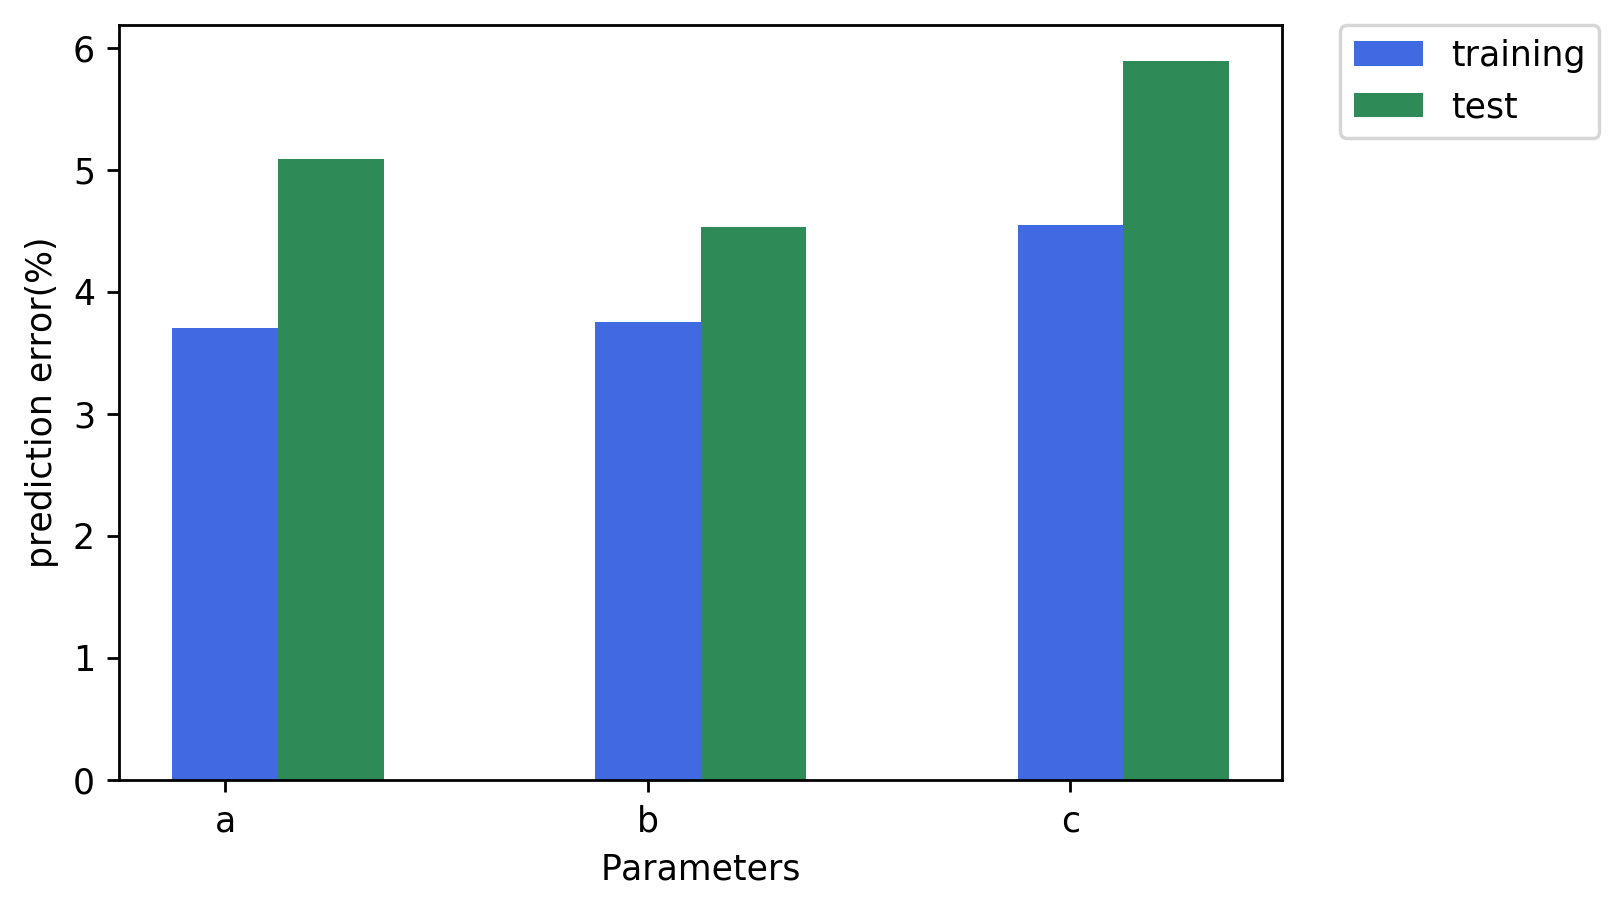
\includegraphics[scale=.45]{images/polyfit/fig_690_params_error.png}
	
	\caption{The error in fitting the parameters $a$, $b$, and $c$ for matrix size $690\times690$.}	
	\label{fig16}
\end{figure}

Using this $3$rd degree polynomial to fit the parameters, we can generalize the relationship between throughput and grain size in the following equation:

\begin{equation}\label{eq3}
P=a_{11}g^2N^3+a_{10}g^2N^2+...+a_1N+a_0
\end{equation}
where $P$ is the throughput, $g$ is the grain size, and $N$ is the number of cores and coefficients $a_{11},...,a_0$ are the real values.

Knowing that a polynomial of degree $2$ in terms of grain size and of degree $3$ in terms of number of cores, we can try to fit our original data directly to the above mentioned formula (Equation~\ref{eq3}). The results of the original data obtained from running $DMATDMATADD$ benchmark, the fitted polynomial based on Equation~\ref{eq3}, is represented in Figure~\ref{fig18}, for 2,4, and 8 cores for a matrix of size $690\times690$.

\vspace{\baselineskip}	
\begin{figure}[H]
	\centering
	\subfloat[]{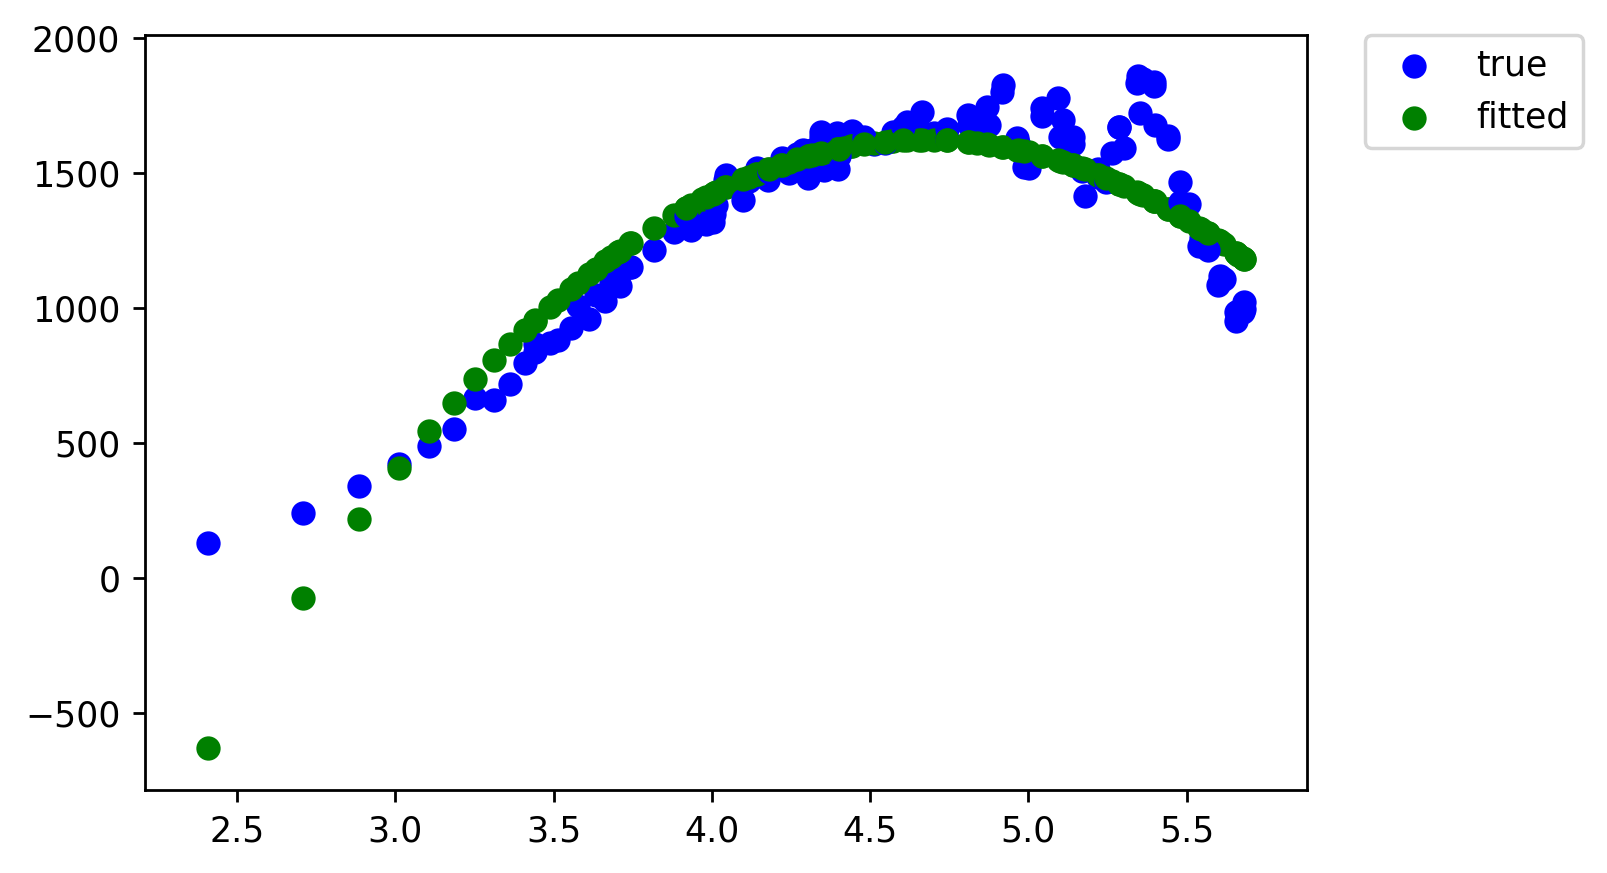
\includegraphics[scale=.35]{images/polyfit/fig_690_total_2.png}\label{fig18:a}}
	\subfloat[]{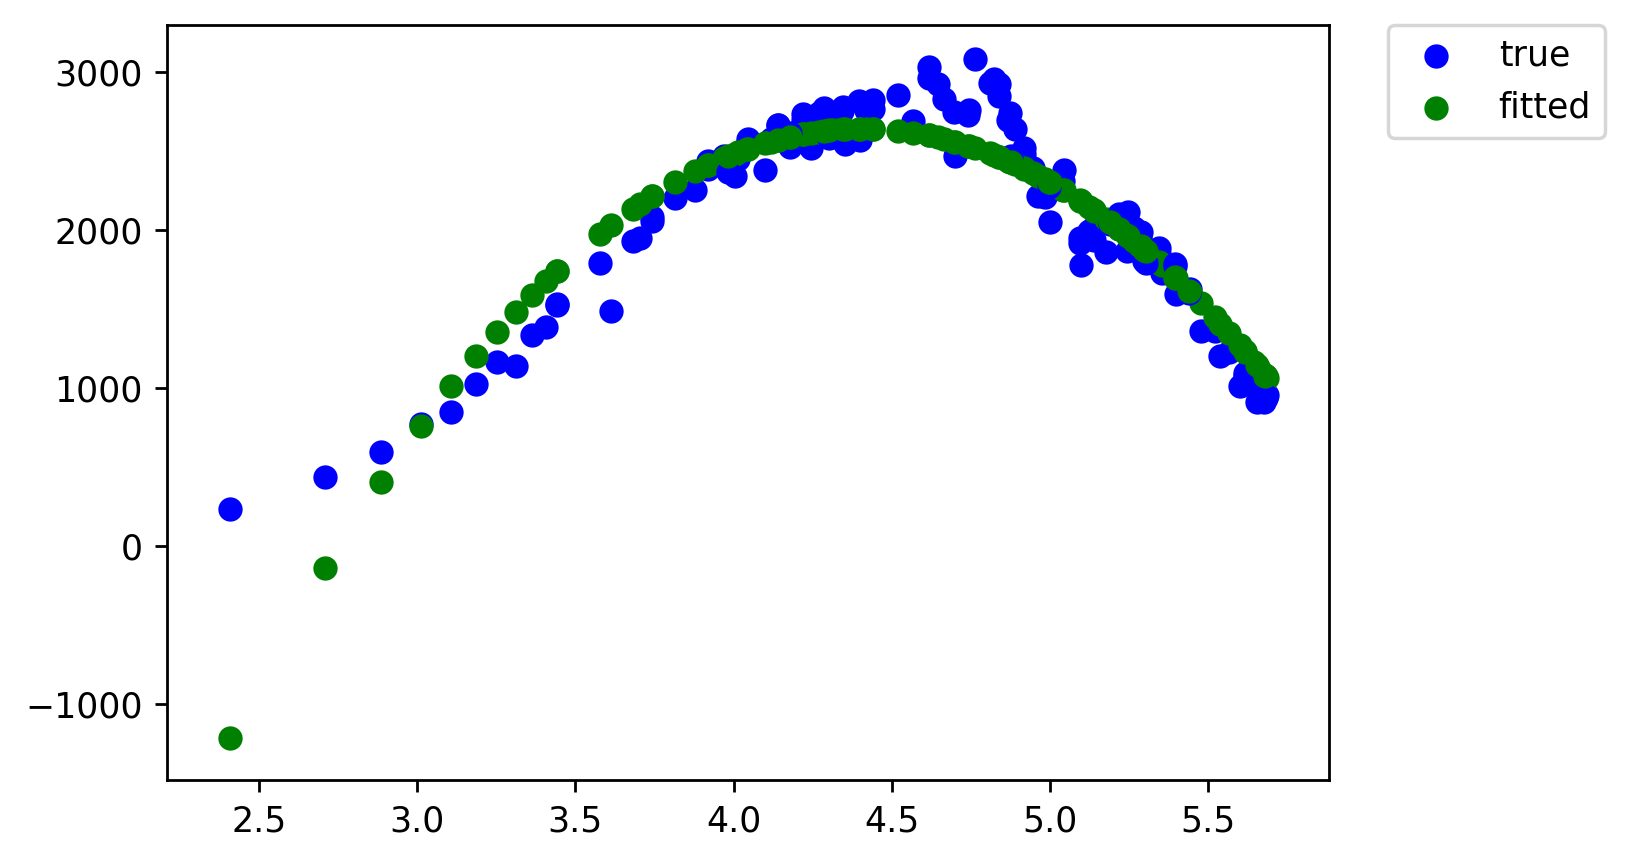
\includegraphics[scale=.35]{images/polyfit/fig_690_total_4.png}\label{fig18:b}}
	\subfloat[]{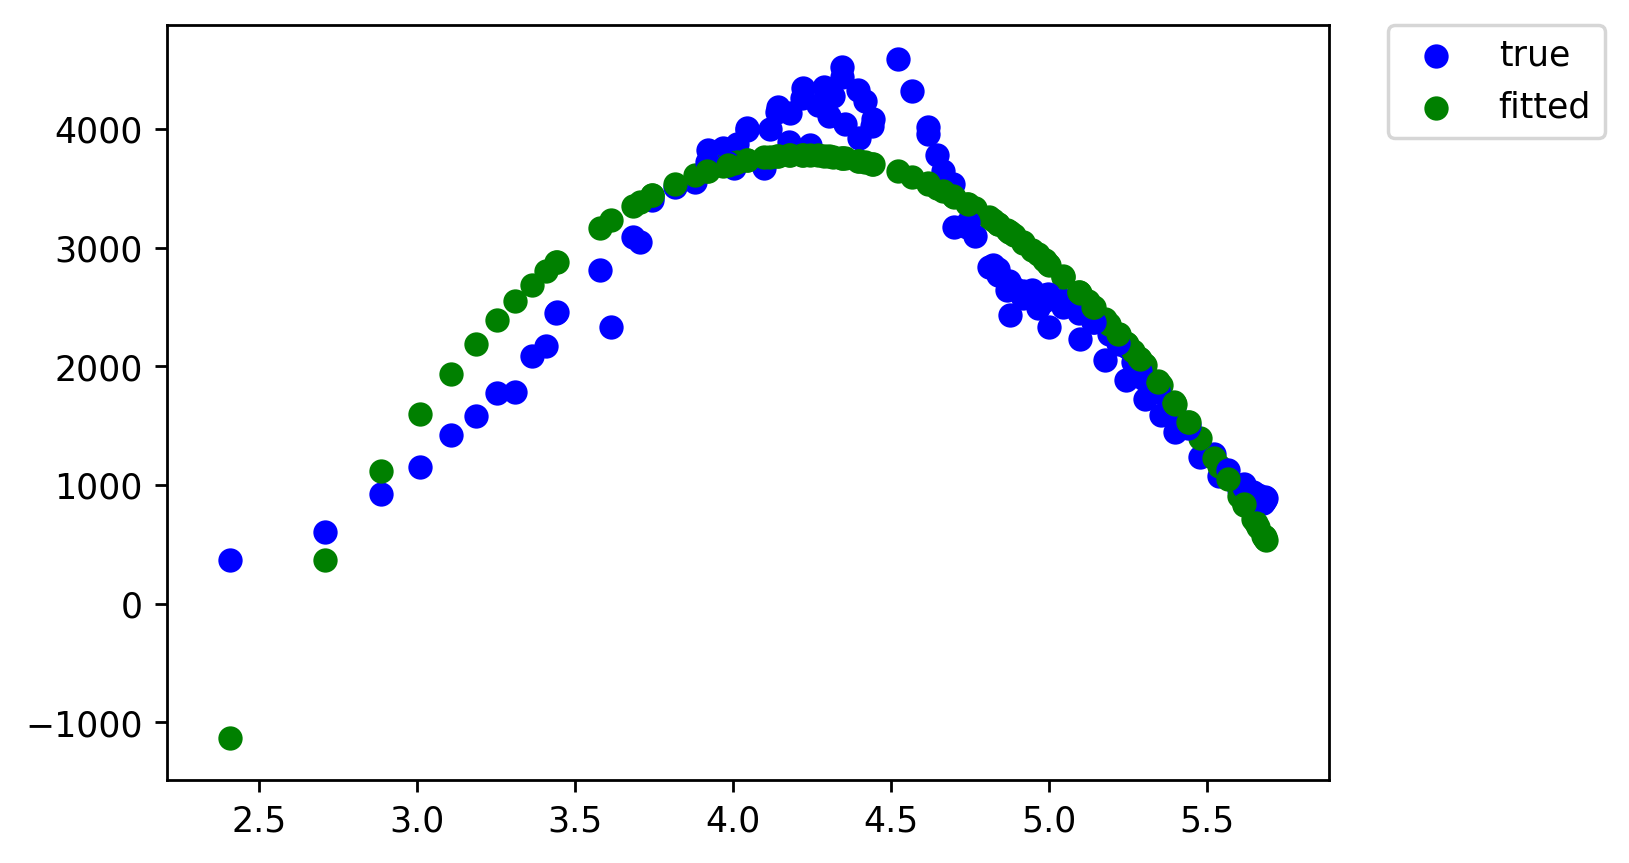
\includegraphics[scale=.35]{images/polyfit/fig_690_total_8.png}\label{fig18:c}}
	\caption{Results of fitting the data from $DMATDMATADD$ benchmark with a polynomial of degree $2$ in terms of grain size and of degree $3$ in terms of number of cores for matrix size $690\times690$ for (a) 2 core, (b) 4 cores, (c) 8 cores.}	
	\label{fig18}
\end{figure}

\vspace{\baselineskip}	
\begin{figure}[H]
	\centering
	\subfloat[]{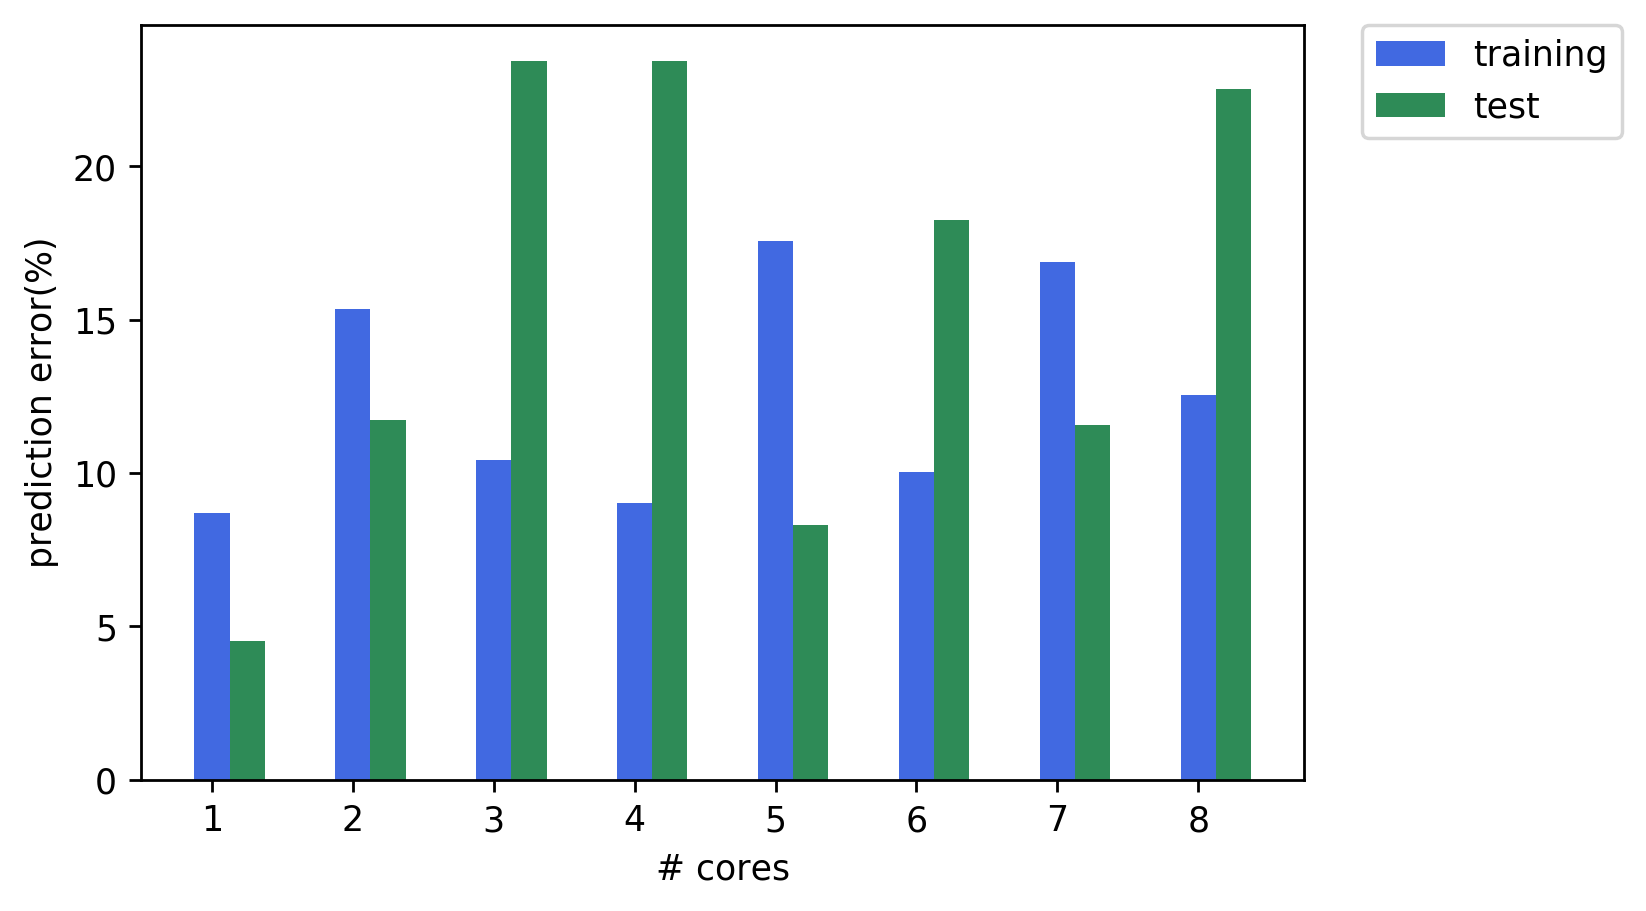
\includegraphics[scale=.45]{images/polyfit/fig_690_total_error.png}\label{fig17:a}}
	\subfloat[]{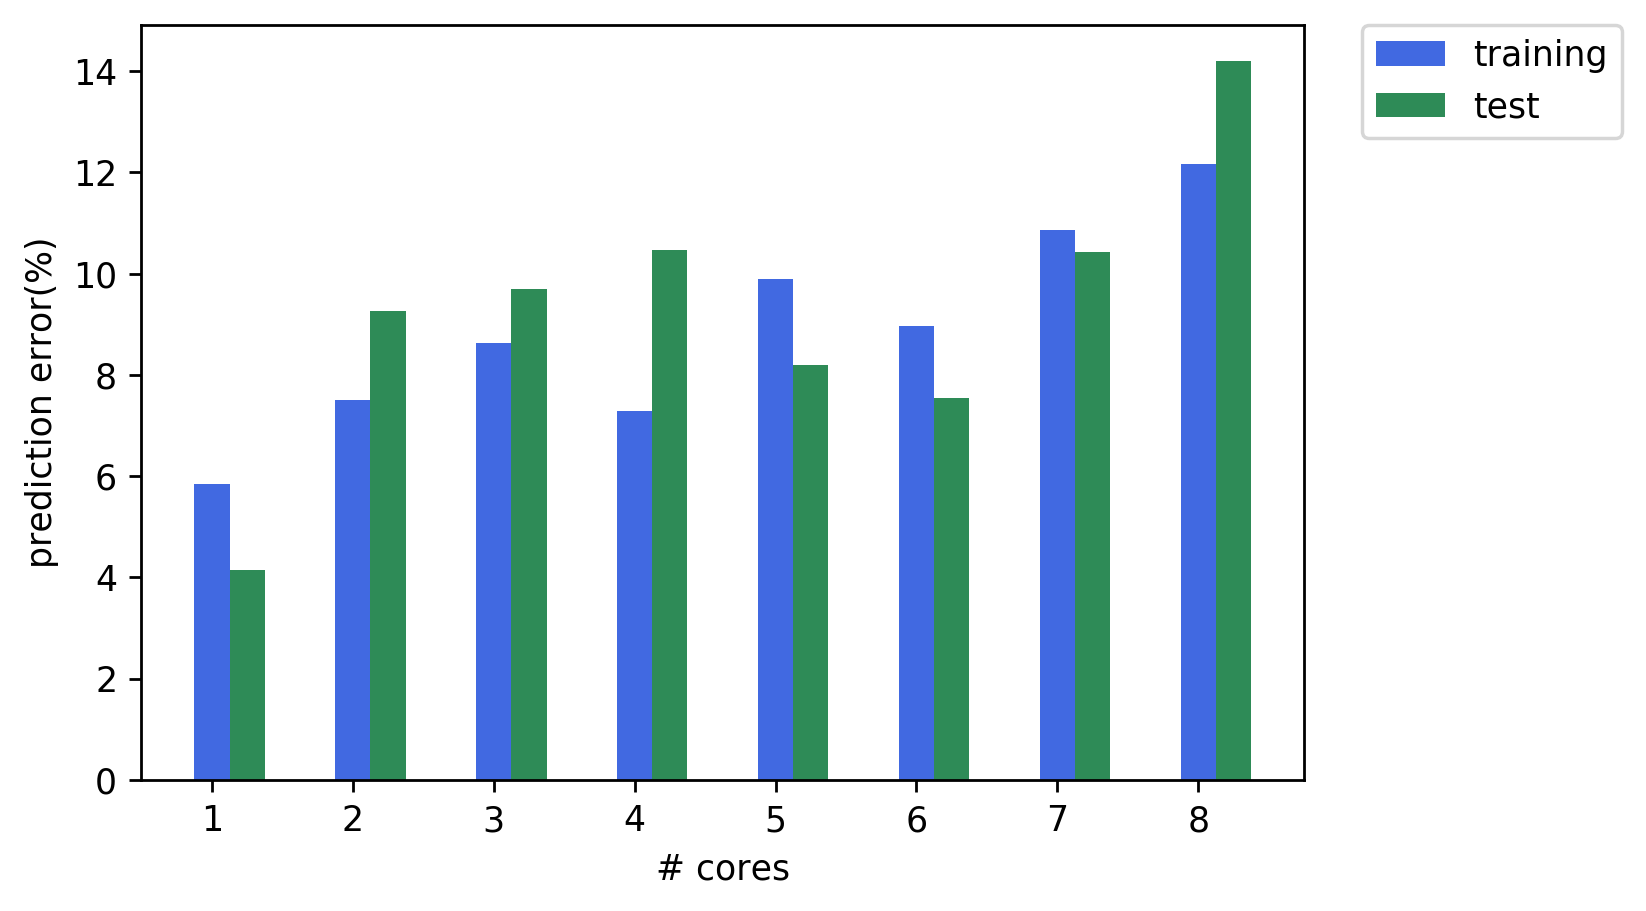
\includegraphics[scale=.45]{images/polyfit/fig_690_total_error_corrected.png}\label{fig17:b}}
	\caption{The training and test error obtained fitting the data to a polynomial of degree $2$ in terms of grain size and of degree $3$ in terms of number of cores for matrix size $690\times690$, for each number of cores. (a) All the data points are include in caluculation of error, (b) the leftmost sample was removed from error calculation.}	
	\label{fig17}
\end{figure}

Figure~\ref{fig17:a} shows the obtained relative error on both training and test sets. The graph suggests a higher test error compared to the training error, mostly caused by the left hand side of the graph. The effect of removing the leftmost sample from error calculations is depicted in Figure~\ref{fig17:b}.

Although we are interested in finding a model that results in a low training and test error, our purpose is mainly finding the region that generates the highest performance. So, even though our model might not match the original data in all data points, due to having a different nature than a quadratic function, our focus would be on how this fit can help us to find which range of grain sizes, or how big the task sizes should be, to achieve the highest performance. 



\vspace{\baselineskip}	
\subsubsection{Finding the range of grain size to achieve high performance}
The major advantage of using a quadratic function to fit the data in terms of grain size, when number of cores is fixed, is the simplicity of the formula, which makes it possible for us to find the peak of the graph very easily. n order to add some uncertainty to our prediction, instead of finding the maximum of the quadratic function, we identified the range of grain size that results in a performance within $10\%$ of the maximum performance. For a second degree polynomial in terms of $g$, $P=ag^2+bg+c$, the minimum or maximum of the polynomial is located at $p^{*}=\frac{-b}{2a}$.    

\vspace{\baselineskip}	
\begin{figure}[H]
	\centering
	\subfloat[]{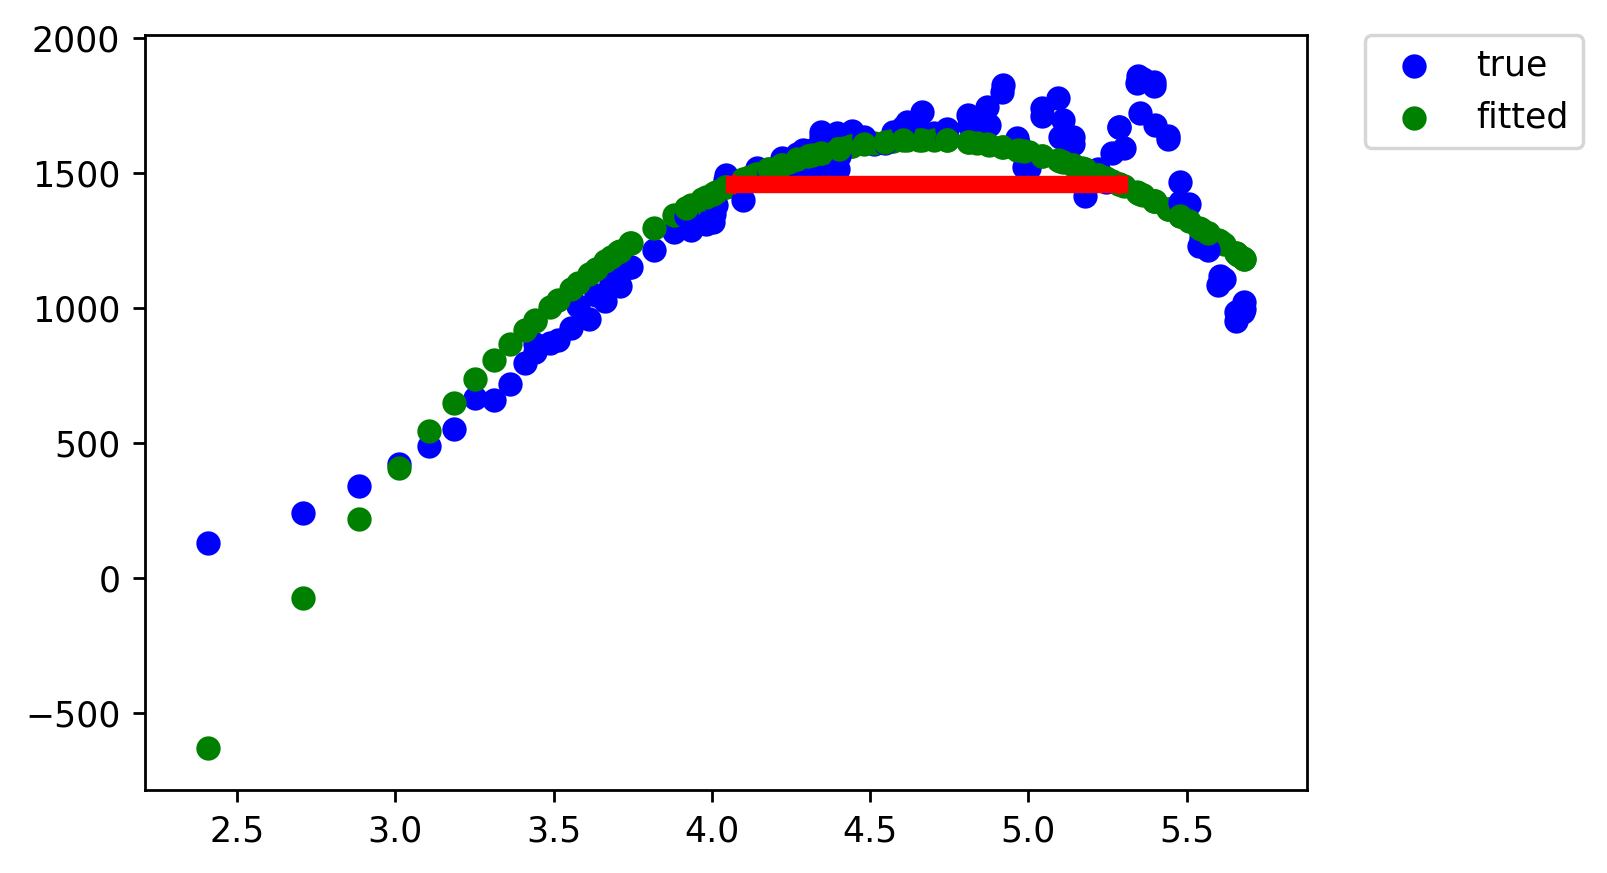
\includegraphics[scale=.3]{images/polyfit/fig_690_total_2_range.png}\label{fig12:a}}
	\subfloat[]{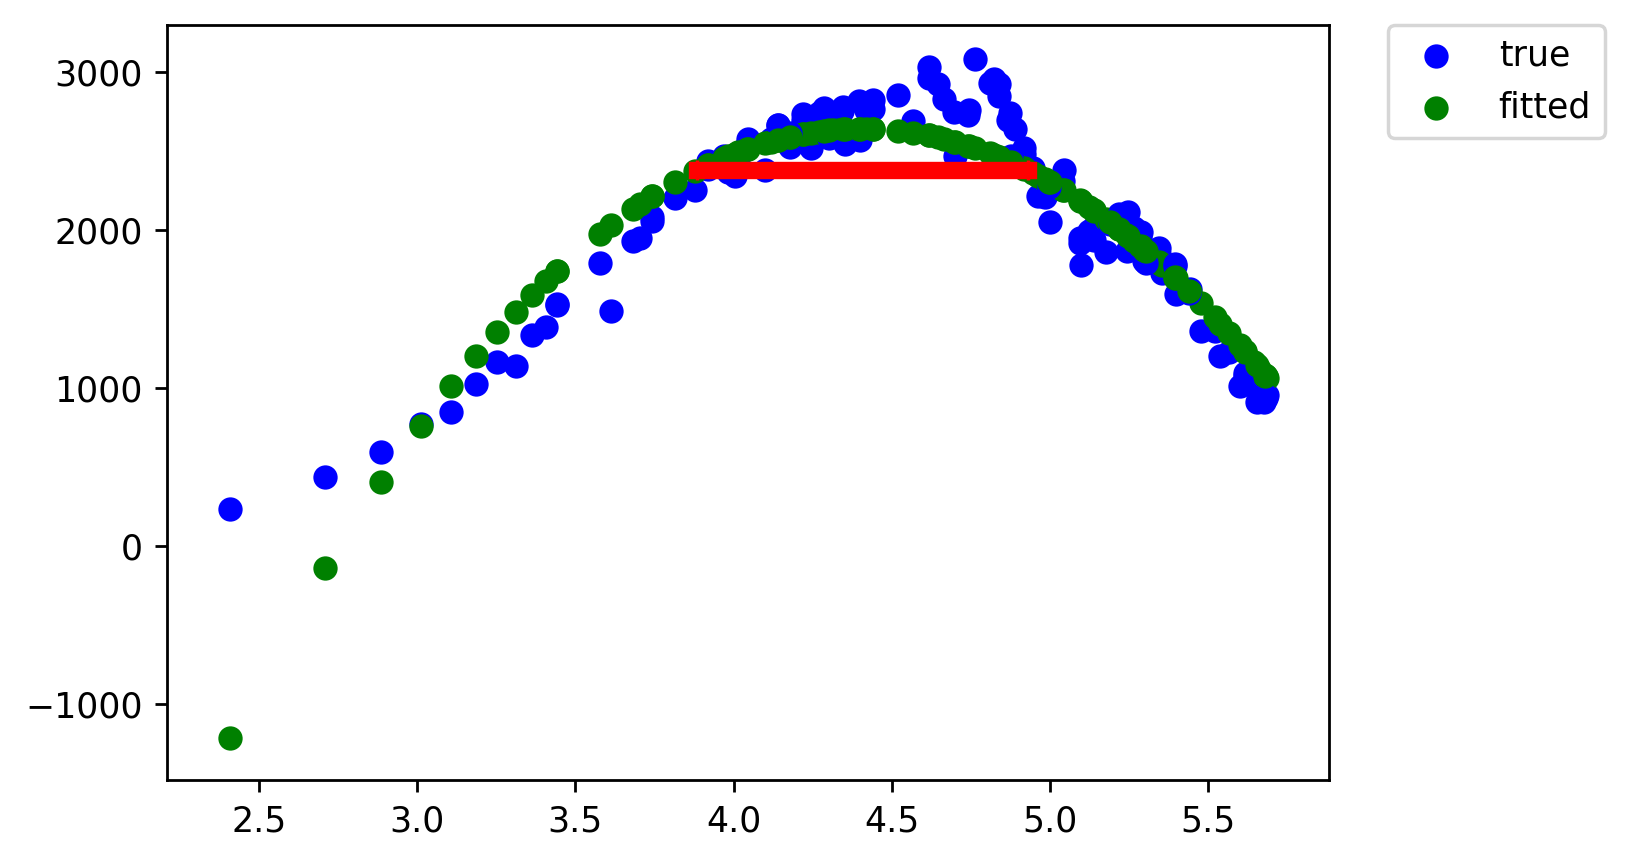
\includegraphics[scale=.3]{images/polyfit/fig_690_total_4_range.png}\label{fig12:b}}
	\subfloat[]{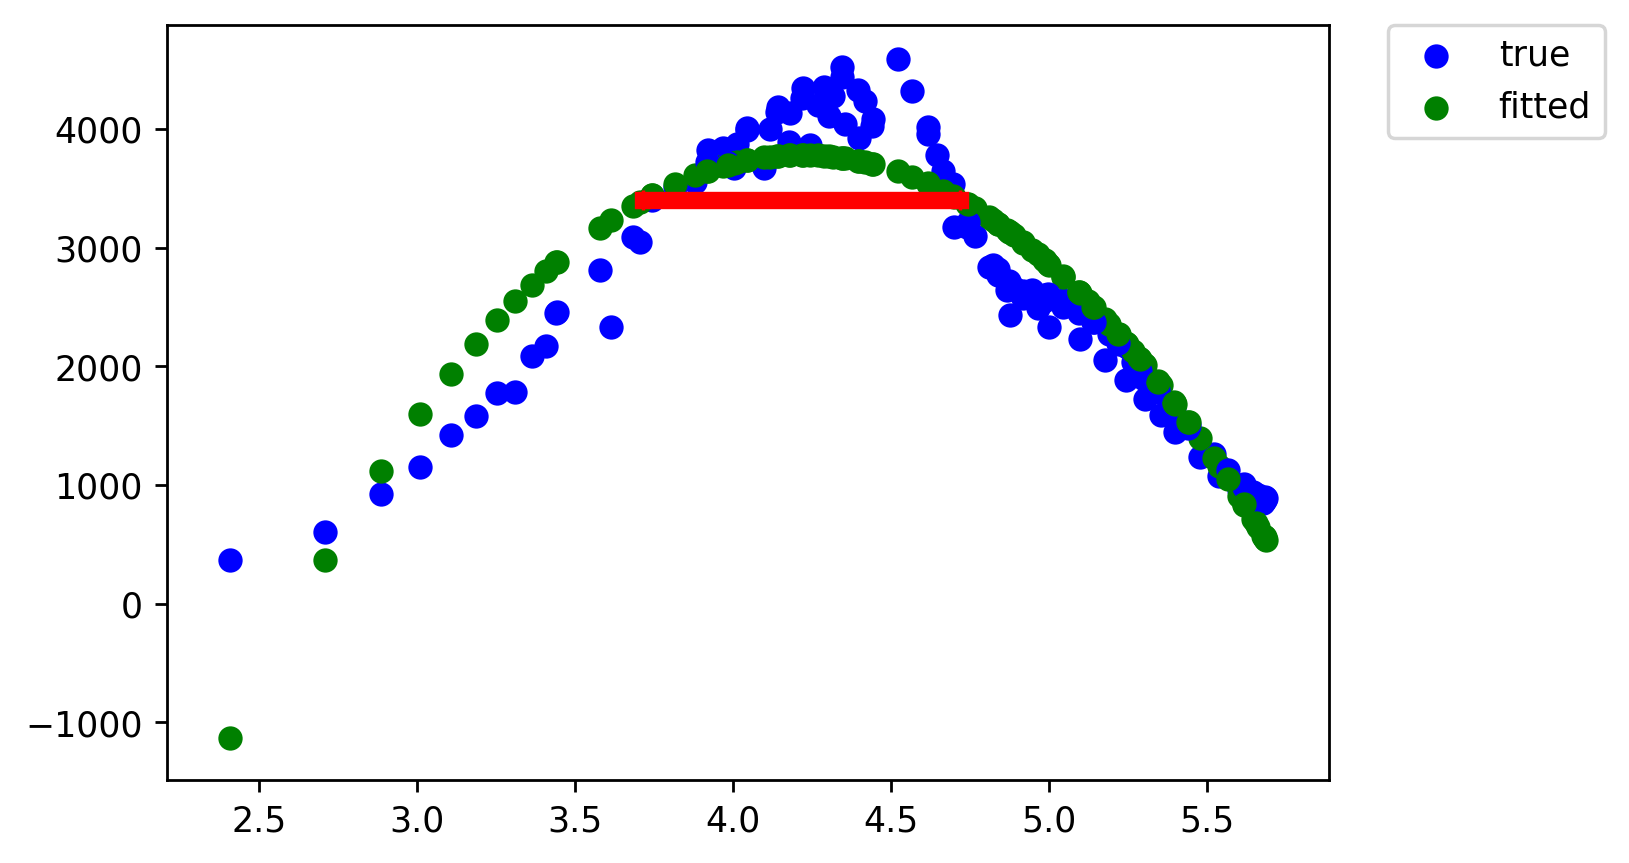
\includegraphics[scale=.3]{images/polyfit/fig_690_total_8_range.png}\label{fig12:c}}
	\caption{The range of grain size (shown as the red line) that leads to a performance within $10\%$ of the maximum performance for (a) 2 cores, (b) 4 cores and (b) 8 cores.}	
	\label{fig12}
\end{figure}


\begin{figure}[H]
	\centering
	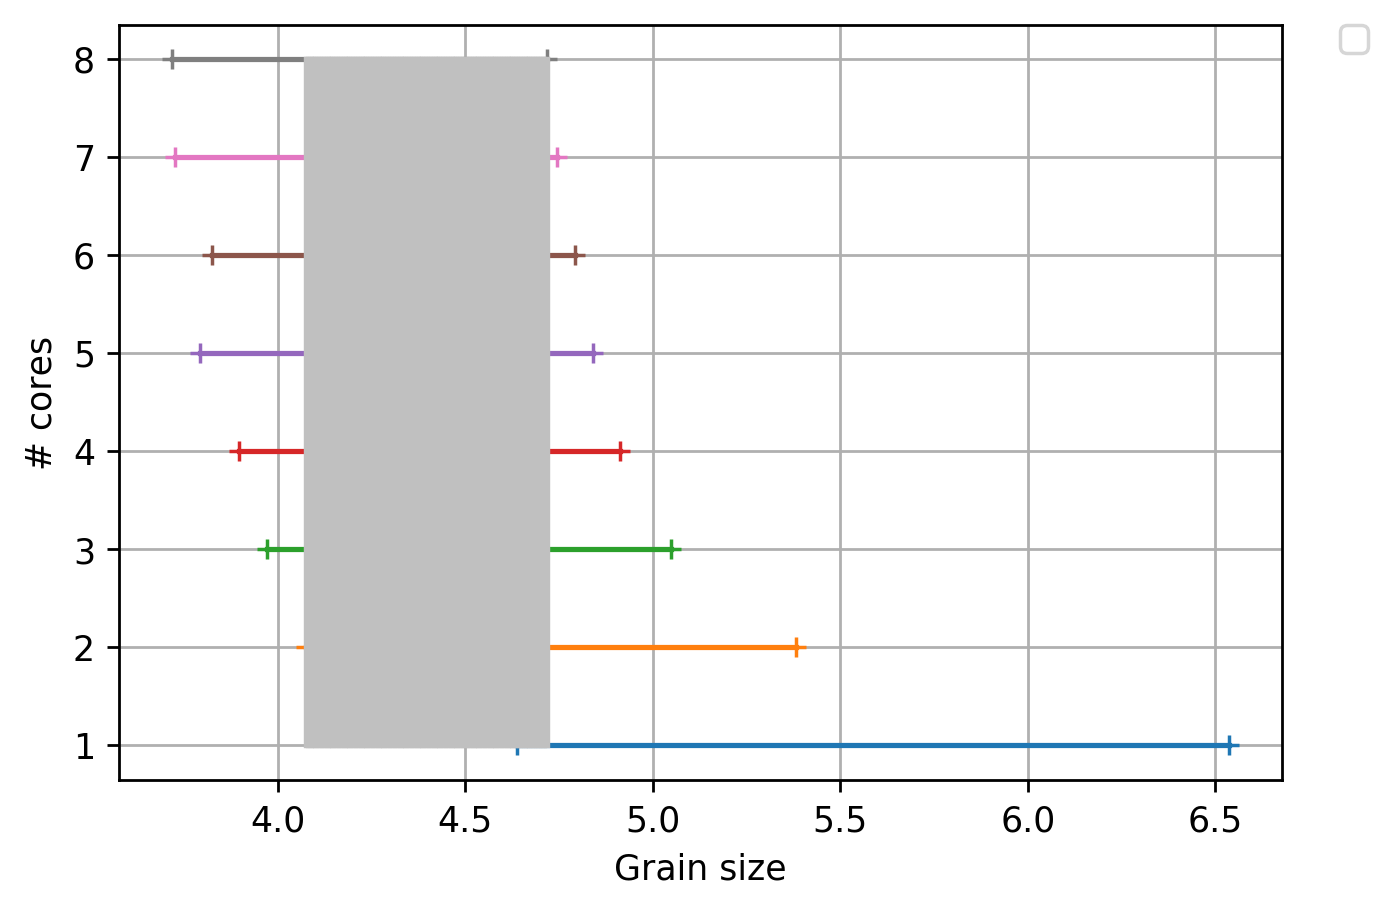
\includegraphics[scale=.75]{images/polyfit/fig_690_peak_range_silver.png}
	\caption{The range of grain size within $10\%$ of the maximum performance of the fitted polynomial function for $DMATDMATADD$ benchmark and matrix size $690\times690$ against different number of cores.}	
	\label{fig13}
\end{figure}



Figure~\ref{fig13} shows the calculated range for matrix size $690\times690$ with different number of threads. In order to generalize the solution, we selected the intersection of all the ranges to find a range of grain size that we expect to work well for all the different number of cores in our experiment. This silver region in Figure~\ref{fig13} corresponds to this range. 
\vspace{\baselineskip}	

\subsubsection{Estimating the chunk size}
Once we identified a range of grain sizes that is expected to leads us to highest achievable performances for a specific matrix size, the next step is finding the possible combinations of block size and chunk size to achieve that range of grain sizes.  
As stated earlier in this chapter, results obtained from Figure~\ref{fig6} suggests that with a fixed grain size, our choice of block size does not affect the performance directly, as long as there exist a chunk size that when combined by the block size could result in the specified grain size. 

In our experiment, we selected our block size to be $4\times256$. With this assumption, in order for the grain size to be within the specified range for each matrix size, chunk size has to be within a specific range size too.

For example, for a $690\times690$ matrix we calculated the range of maximum performance for all number of cores to be $[4.069, 4.719]$ in logarithmic scale which is equivalent to $[11711, 52368]$. Setting the block size to $4\times256$, this range forces the chunk size to be within the range $[13,56]$. The range of chunk sizes to match the range of grain sizes identified, and their corresponding throughput is shown in Figure~\ref{fig14}, for matrix size $690\times690$ and block size $4\times256$. The green line is the throughput achieved by the current implementation of HPX backend. 


  
\vspace{\baselineskip}	
\begin{figure}[H]
	\centering
	\subfloat[]{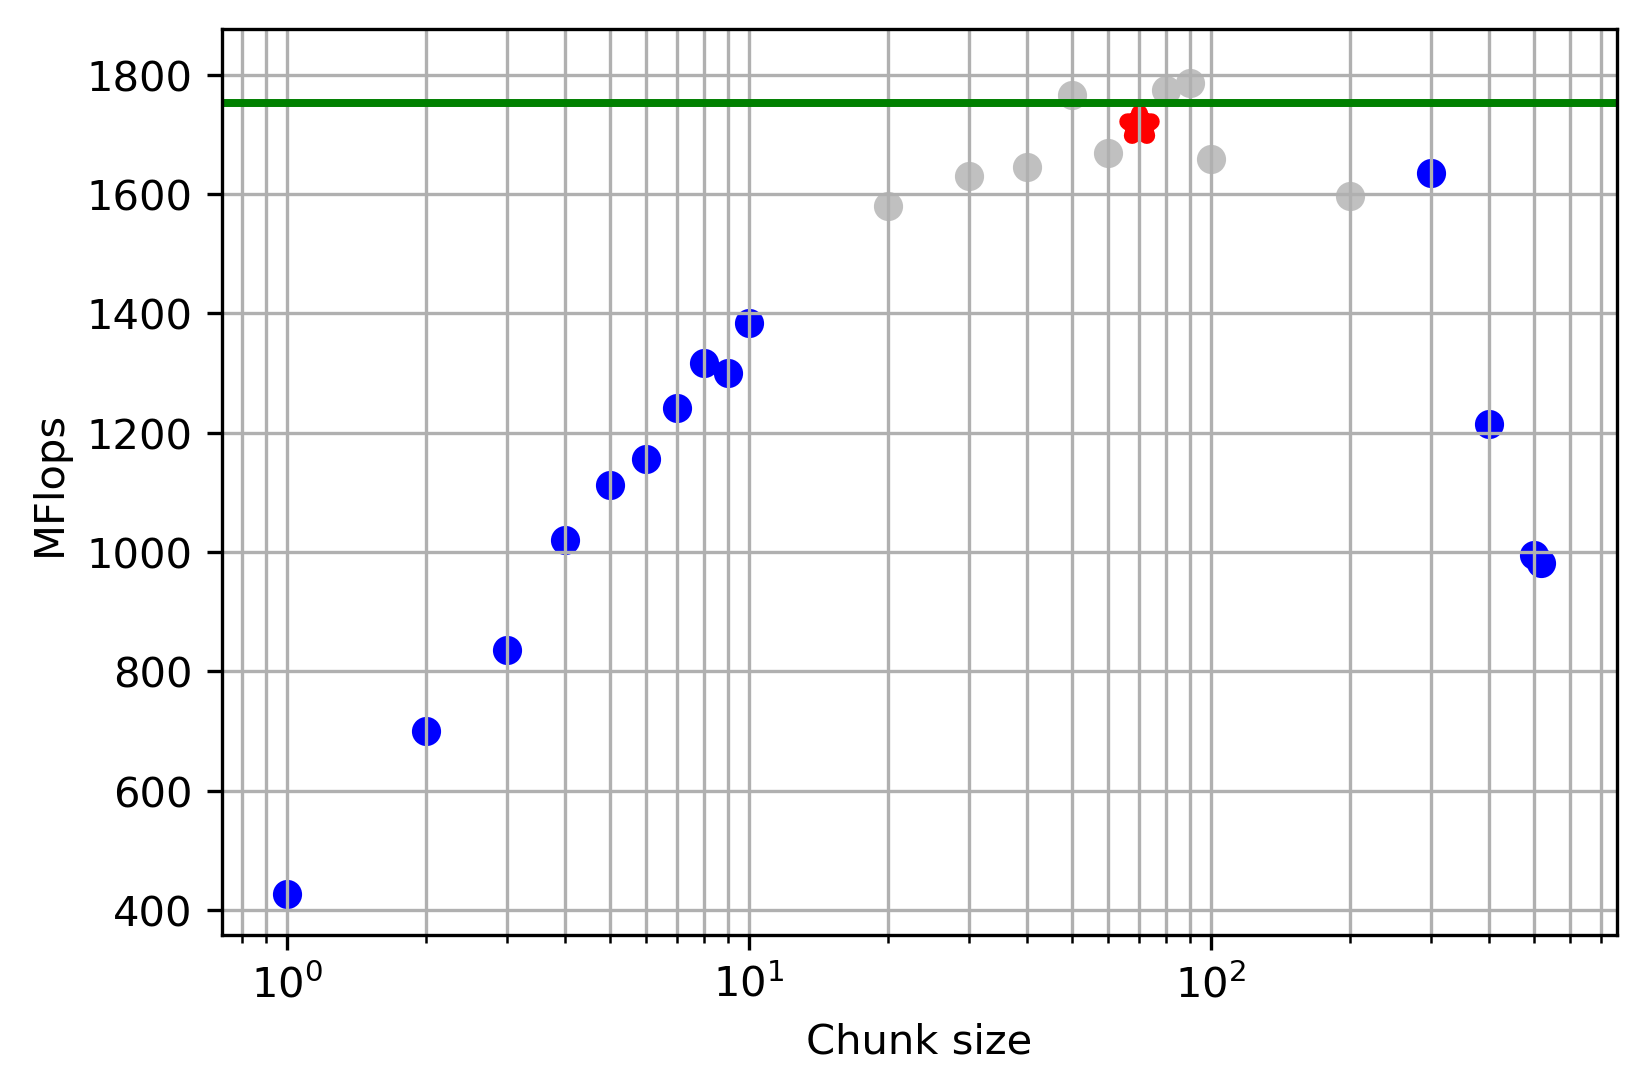
\includegraphics[scale=.35]{images/polyfit/fig_690_chunks_2_4-256.png}\label{fig14:a}}
	\subfloat[]{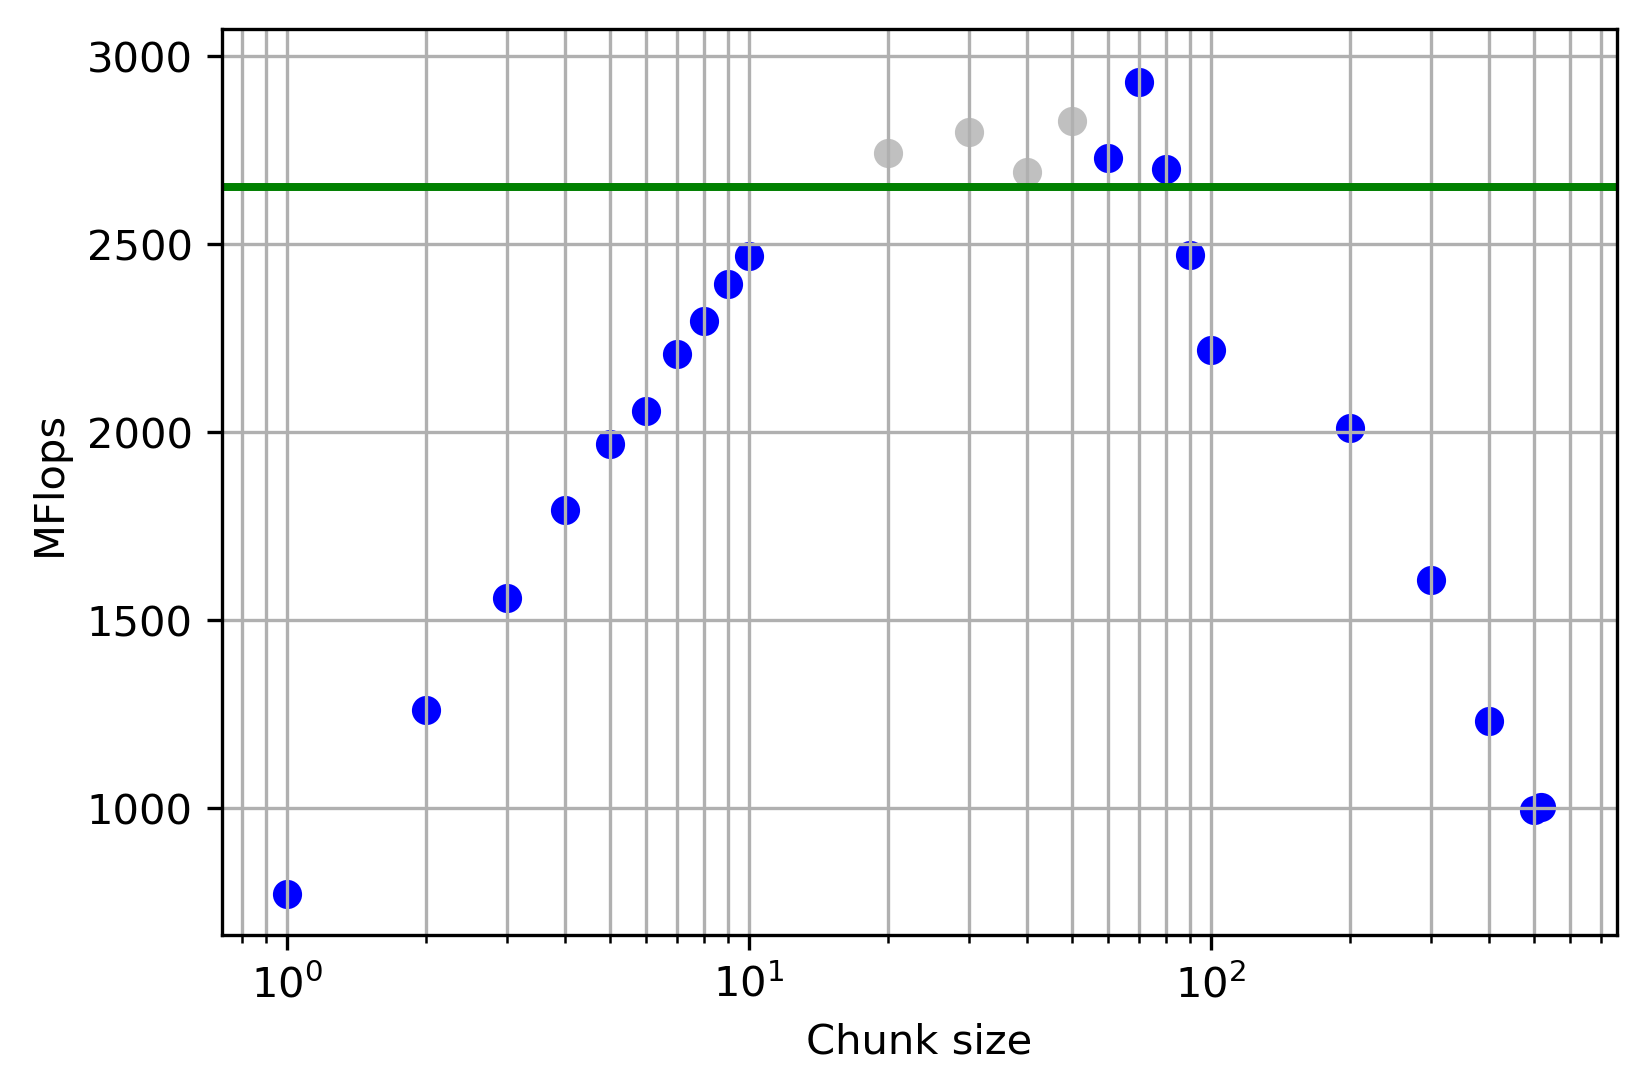
\includegraphics[scale=.35]{images/polyfit/fig_690_chunks_4_4-256.png}\label{fig14:b}}
	\subfloat[]{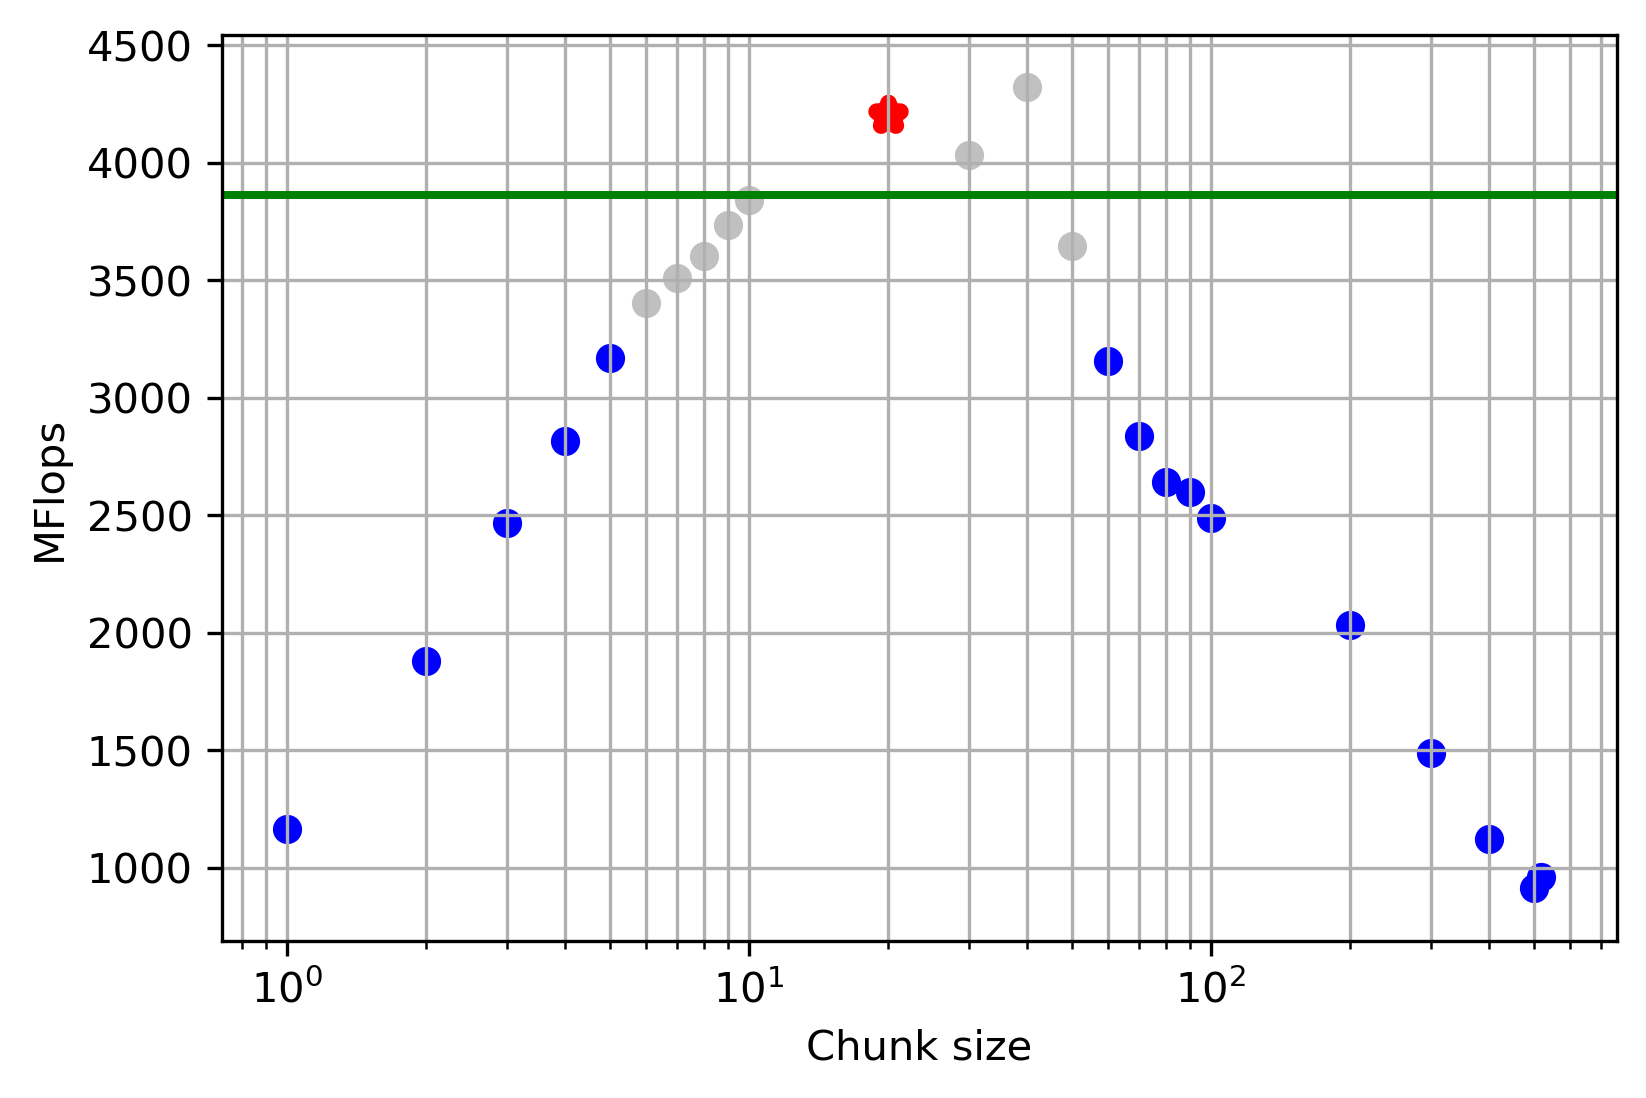
\includegraphics[scale=.35]{images/polyfit/fig_690_chunks_8_4-256.png}\label{fig14:c}}
	\hfill
	\subfloat[]{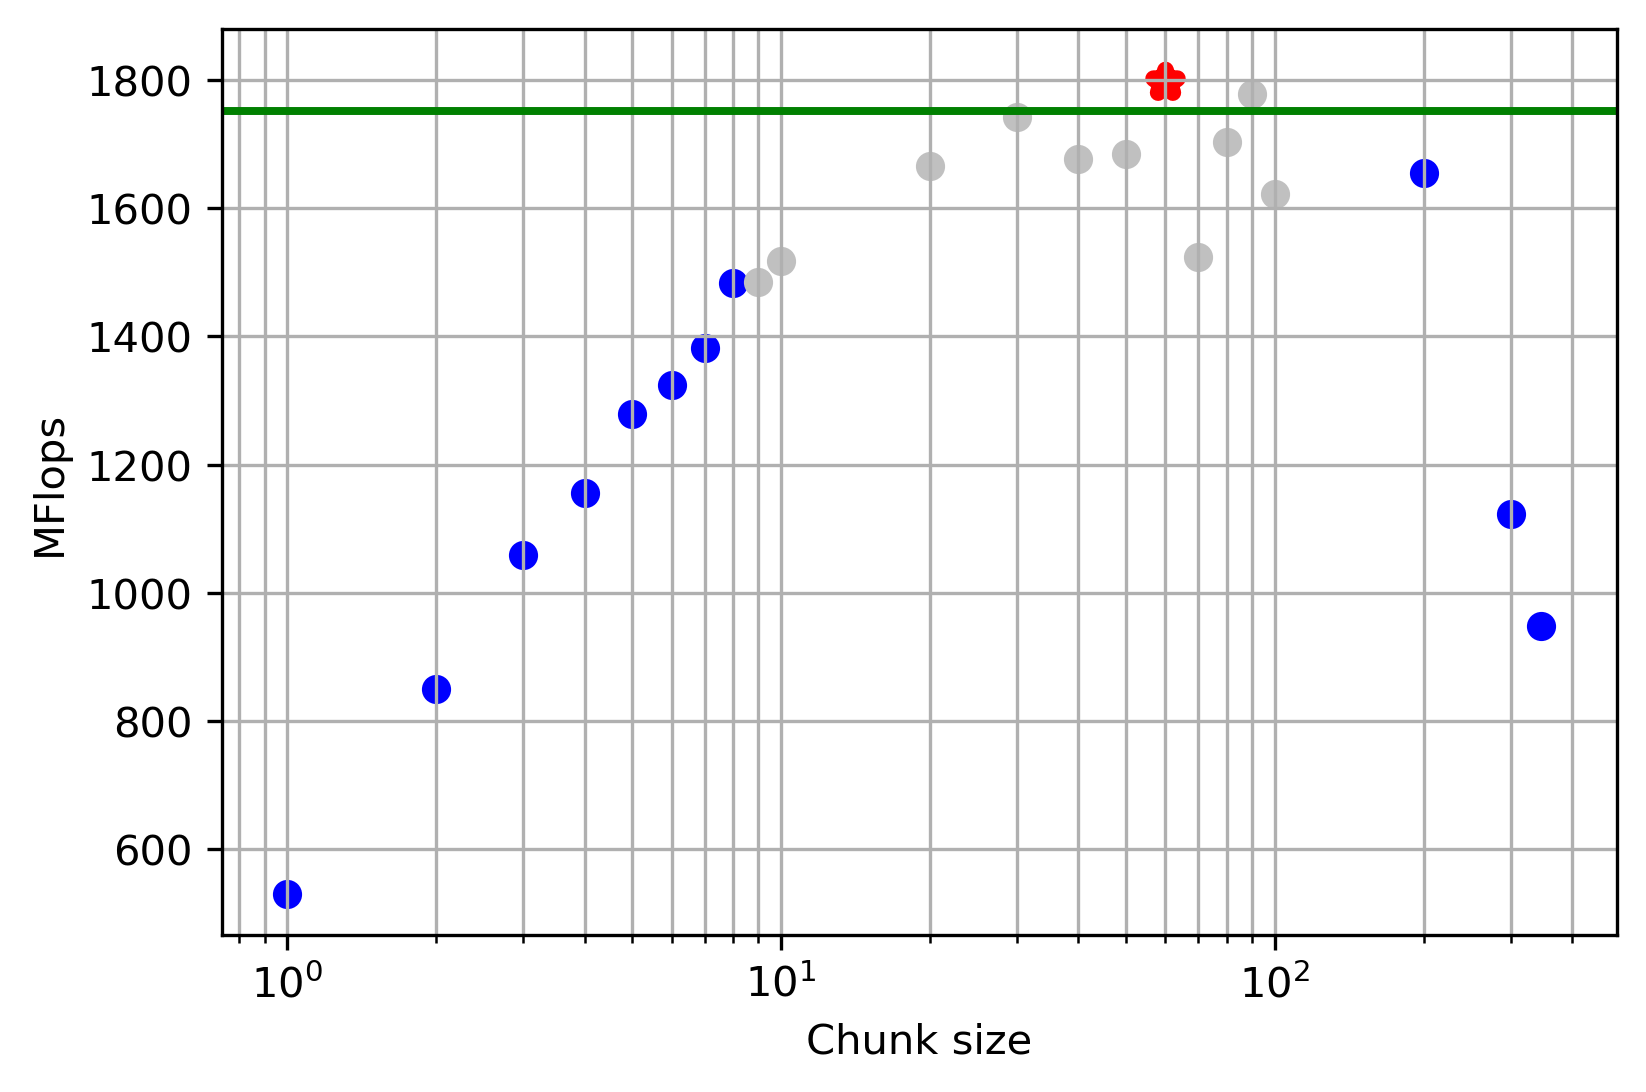
\includegraphics[scale=.35]{images/polyfit/fig_690_chunks_2_4-512.png}\label{fig14:d}}
	\subfloat[]{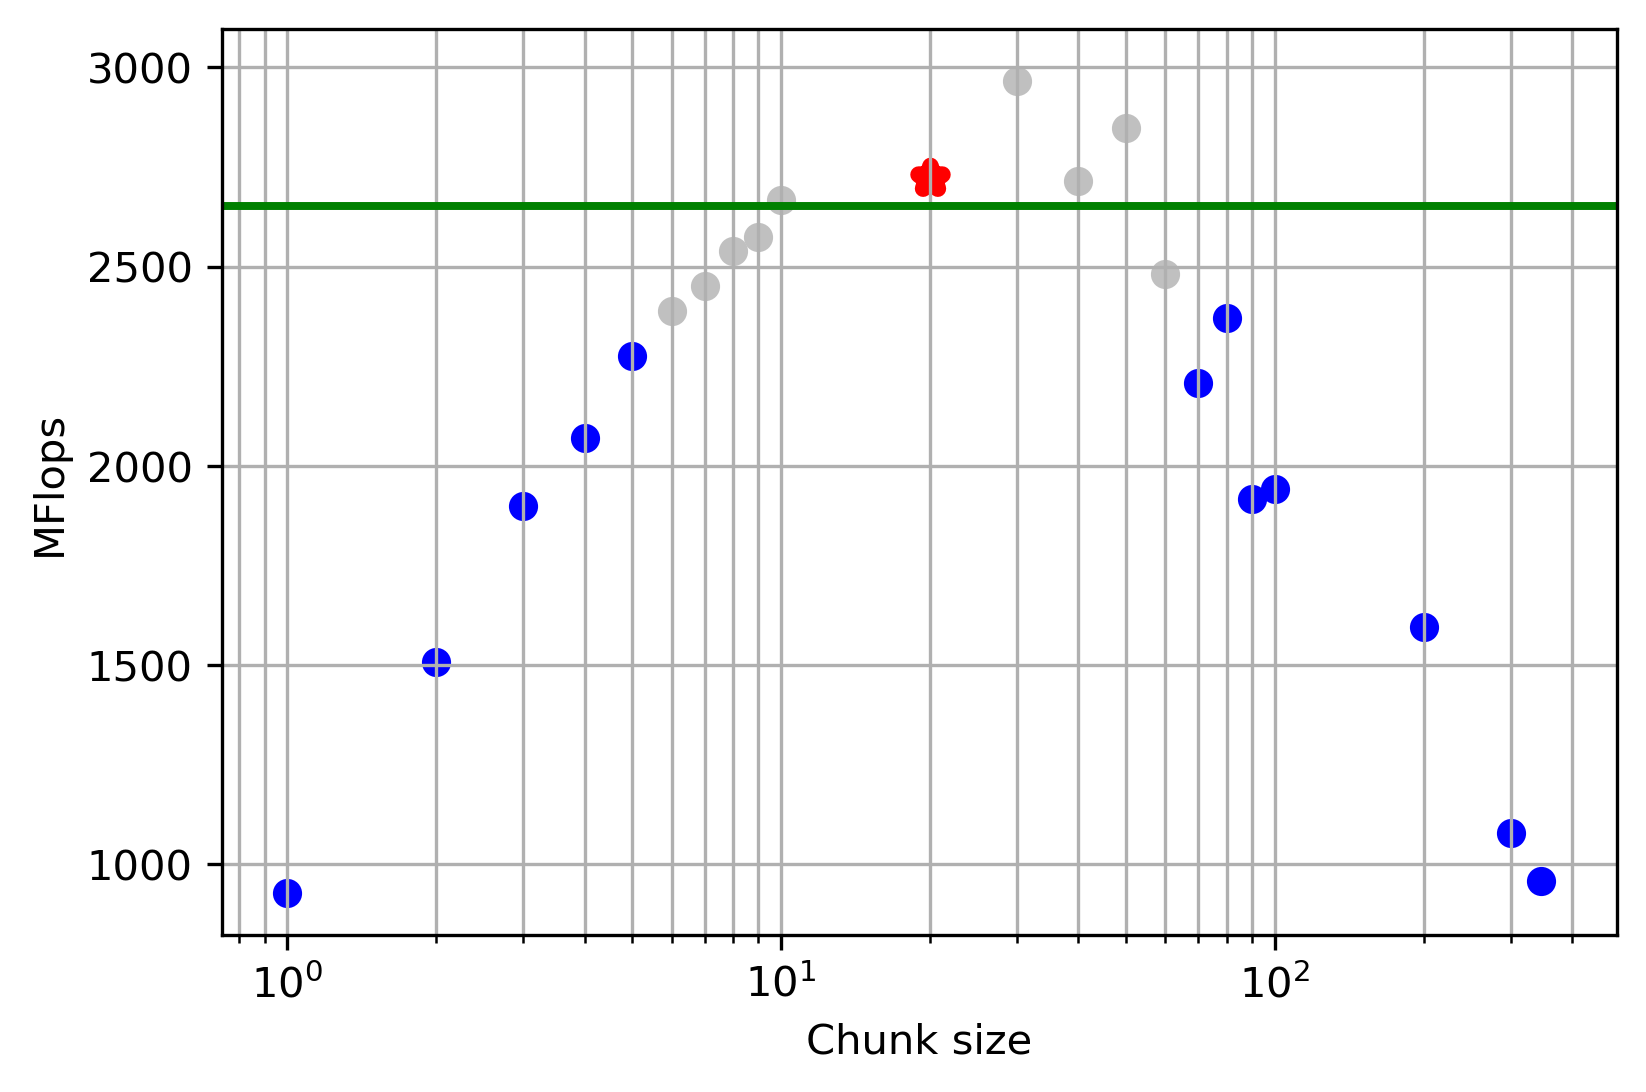
\includegraphics[scale=.35]{images/polyfit/fig_690_chunks_4_4-512.png}\label{fig14:e}}
	\subfloat[]{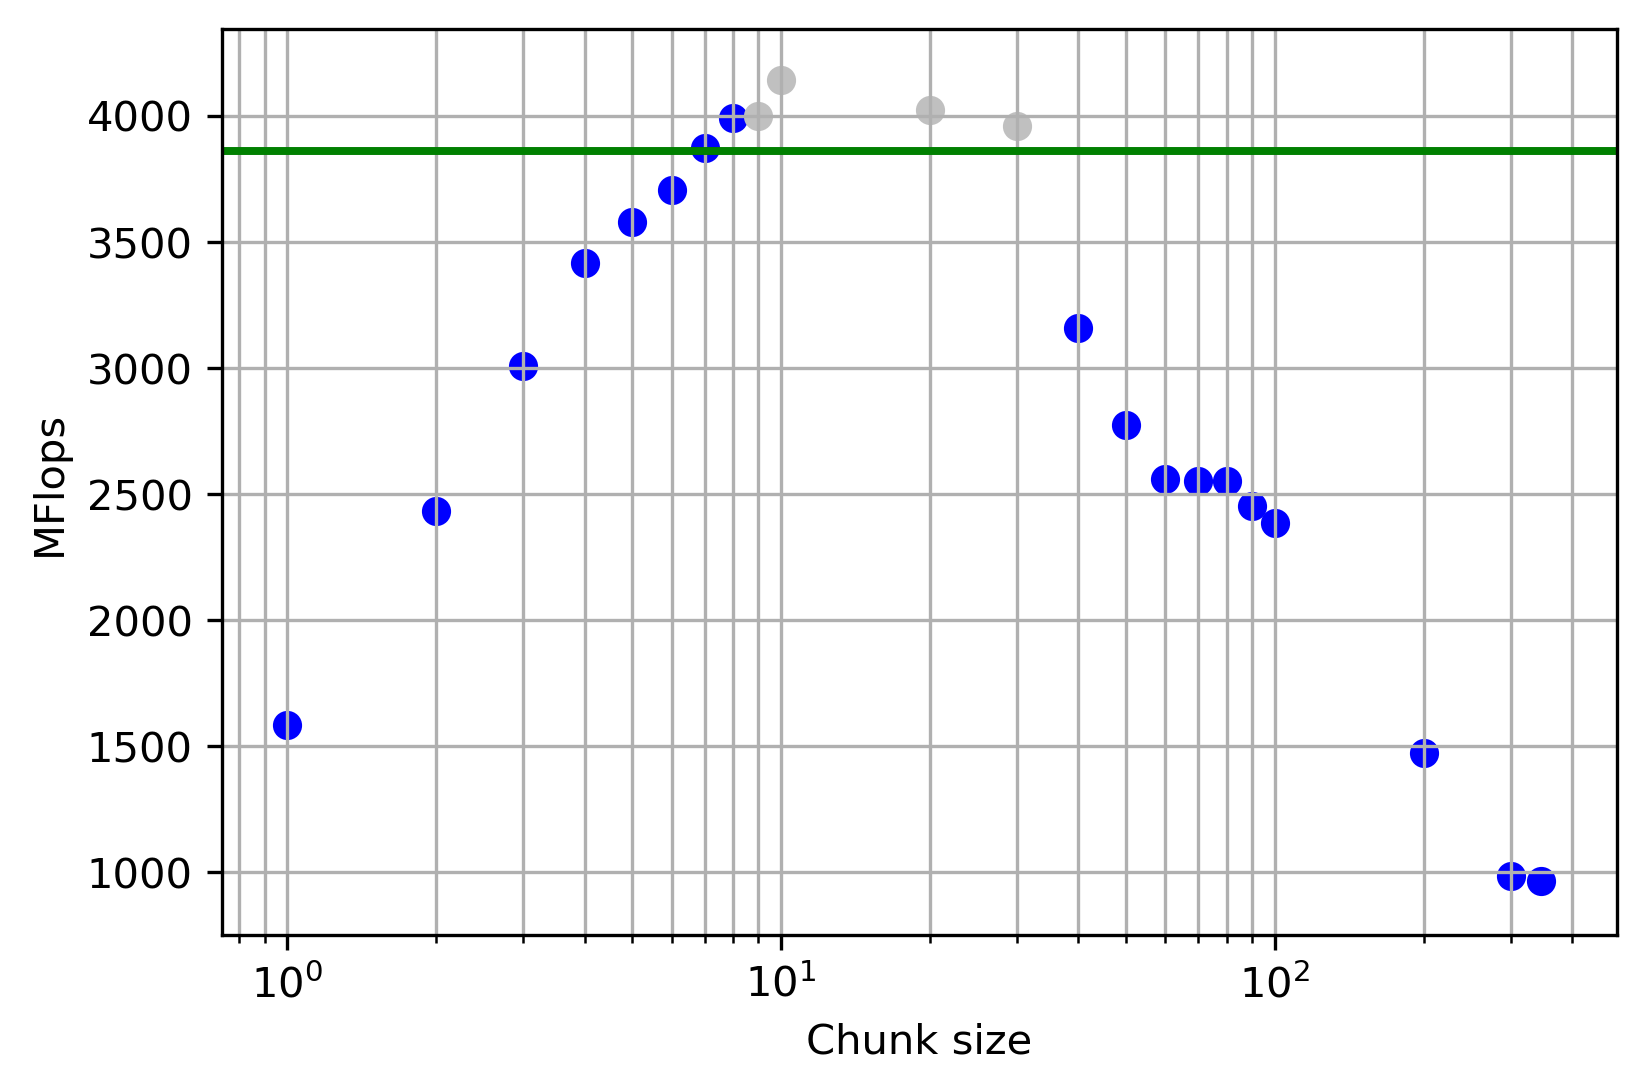
\includegraphics[scale=.35]{images/polyfit/fig_690_chunks_8_4-512.png}\label{fig14:f}}
	\caption{The range of chunk sizes to produce a grain size within $10\%$ of the maximum performance of the fitted quadratic function for $DMATDMATADD$ benchmark for matrix size $690\times690$ with block size of $4\times256$ on (a) $2$ cores, (b) $4$ cores, and (c) $8$ cores, and block size of $4\times512$ on (d) $2$ cores, (e) $4$ cores, and (f) $8$ cores. Silver points denotes the detected range of chunk size.}	
	\label{fig14}
\end{figure}


\subsection{Bathtub fit}
In the previous section we studied the possibility of using a polynomial to capture the relationship between grain size, number of cores, and throughput for a fixed matrix size, with the purpose of finding a range of grain size that leads us to maximum performance. 
Although the polynomial function was helpful in directing us toward our objective, it does not have a physical implication. 

This motivated us to change our view, and instead of looking just at the data and trying to find a function to fit the data, study the behavior of the data, and then find a function that would be likely to fit the data. That function would be a good fit mostly because that's how we expect the throughput to change with grain size, and not just how the data looks like.   


